\documentclass{article}\usepackage[]{graphicx}\usepackage[]{color}
%% maxwidth is the original width if it is less than linewidth
%% otherwise use linewidth (to make sure the graphics do not exceed the margin)
\makeatletter
\def\maxwidth{ %
  \ifdim\Gin@nat@width>\linewidth
    \linewidth
  \else
    \Gin@nat@width
  \fi
}
\makeatother

\definecolor{fgcolor}{rgb}{0.345, 0.345, 0.345}
\newcommand{\hlnum}[1]{\textcolor[rgb]{0.686,0.059,0.569}{#1}}%
\newcommand{\hlstr}[1]{\textcolor[rgb]{0.192,0.494,0.8}{#1}}%
\newcommand{\hlcom}[1]{\textcolor[rgb]{0.678,0.584,0.686}{\textit{#1}}}%
\newcommand{\hlopt}[1]{\textcolor[rgb]{0,0,0}{#1}}%
\newcommand{\hlstd}[1]{\textcolor[rgb]{0.345,0.345,0.345}{#1}}%
\newcommand{\hlkwa}[1]{\textcolor[rgb]{0.161,0.373,0.58}{\textbf{#1}}}%
\newcommand{\hlkwb}[1]{\textcolor[rgb]{0.69,0.353,0.396}{#1}}%
\newcommand{\hlkwc}[1]{\textcolor[rgb]{0.333,0.667,0.333}{#1}}%
\newcommand{\hlkwd}[1]{\textcolor[rgb]{0.737,0.353,0.396}{\textbf{#1}}}%
\let\hlipl\hlkwb

\usepackage{framed}
\makeatletter
\newenvironment{kframe}{%
 \def\at@end@of@kframe{}%
 \ifinner\ifhmode%
  \def\at@end@of@kframe{\end{minipage}}%
  \begin{minipage}{\columnwidth}%
 \fi\fi%
 \def\FrameCommand##1{\hskip\@totalleftmargin \hskip-\fboxsep
 \colorbox{shadecolor}{##1}\hskip-\fboxsep
     % There is no \\@totalrightmargin, so:
     \hskip-\linewidth \hskip-\@totalleftmargin \hskip\columnwidth}%
 \MakeFramed {\advance\hsize-\width
   \@totalleftmargin\z@ \linewidth\hsize
   \@setminipage}}%
 {\par\unskip\endMakeFramed%
 \at@end@of@kframe}
\makeatother

\definecolor{shadecolor}{rgb}{.97, .97, .97}
\definecolor{messagecolor}{rgb}{0, 0, 0}
\definecolor{warningcolor}{rgb}{1, 0, 1}
\definecolor{errorcolor}{rgb}{1, 0, 0}
\newenvironment{knitrout}{}{} % an empty environment to be redefined in TeX

\usepackage{alltt}

\usepackage[backend=bibtex, sorting=none, citestyle=authoryear]{biblatex}
\usepackage[margin=0.8in]{geometry}
\bibliography{references}


\usepackage{draftwatermark}
\SetWatermarkText{DRAFT}
\SetWatermarkScale{5}
\SetWatermarkLightness{0.95}

\title{Efficiency}
\author{Aidan Morrison}
\IfFileExists{upquote.sty}{\usepackage{upquote}}{}
\begin{document}

\maketitle




Para

\tableofcontents

\section{Introduction}

The purpose of this paper is to investigate the suitability of the pump-jet selection for Australia's future fleet of submarines.  In particular, the question of the relative efficiency, and quietness of pump-jets in comparison to open propellers is of particular importance.  Much has been made of the significance of the pump-jet in the DCNS (now Naval Group) bid for the submarine, to the extent that it has been claimed that the pump-jet rendered propellers obsolete.

Necessarily, this topic depends upon a considerable amount of physics, particularly around hydrodynamics, fluid mechanics, and turbomachinery, all of which might be difficult or daunting topics to usefully inform a public policy debate. However, in the case of a \$50 billion dollar military acquisition, neglecting to engage with the technical matters that are so crucial to such a decision would be deeply foolish.  To that end, this paper has a very specific ambition.  It doesn't seek to advance the technical field with any new research or insight.  Instead, it aims to make as much of the relvant physics as possible to this particular question comprehensible in laymans terms, and connect the essential concepts as directly as possible with the most important conclusions of public import.

As such, it will tend to make frequent use of diagrams, illustrations, as well as simple prose, and relatively infrequently use mathematical equations, (unless of crucial importance), though some effort is made to point to references where the fuller and more formal derivations of these relationships can be found.

It should be noted that the technical fields involved here are vast and rapidly evolving.  The author makes no claim to be a world authority on the entirety of the topics which are touched. It is quite possible that there are other effects and phenomena which could be relevant which aren't mentioned here, and it's also true that additional advances in the state of the art are being made continually, and might not be known about in public literature.

However, the nature of scientific discovery and technical progress is that many of best discoveries are actually built-upon and confirmed, rather than swept aside, by later developments.  As such, plenty of foundational principals, in particular the conservation laws of energy and momentum and essential principals of mechanics and thermodynamics are just as true, right, and relevant as they were hundreds of years ago.  Consequently, whilst we cannot always know the precise degree of advance in a particular field of engineering, we can still confidently know some of the fundamental bounds and constraints that will be inherent in that field.

In this paper, since we cannot know the precise details of the particular state of the art in largely classified military programs, I will attempt to be particularly clear about those things for which we can have great confidence (often broad principals or relationships which determine trade-offs) and those things which we can't (the precise degrees or points and sensitivities).  To that end, in this paper I've underaken modelling based upon the broad principals which we can have confidence, and conducted sensitivity testing based on a range of plausible values which seem realistic for those things about which we can have less confidence. I have also, in discussion with experts and through reading the available literature, attempted where possible to identify the most plausible of the uncertain values, in order to advance discussion.

With the support of the principal sponsor of this paper, the relevant models may be found in a user-friendly format as a web-app to allow their further interrogation and testing for other plausible scenarios.  In addition, for increased transparency, the relevant code and equations underlying are available on github.

\section{Executive Summary}

\subsection{The difference between nuclear and conventional for speed}
This paper was commissioned in order to investigate whether pumpjets could plausibly be as efficient, or more efficient than a suitably designed open propeller for a conventional submarine. A crucial input to the investigation is a rough understanding of what the speeds of operation are likely to be for a submarine.  Whereas nuclear submarines are reportedly capable of reaching speeds in excess of 30kt, and might transit long distances at such high speeds, conventional sumbarines are not thought of as being able to reach speeds far above 20kt in a sprint, and can only sustain speeds of 8-10kt for long-distance transits.  Moreover, on patrol, a large portion of thier work is done at very low speeds, typically thought to be in the range of 2-4kt.

\subsection{The importance of low speed operation for diesel-electric submarines}
The efficiency of the propulsion system at such low speeds is of great significance for a conventional submarine, since it must rely on batteries or other air-independent propulsion sources for power when entirely submerged.  Consequently, excessive energy consumption results in greatly reduced dived endurances.  Since a submarine's position is vastly more likely to be discovered when it is on the surface operating its diesel engines, this ability to remain submerged for a long time is crucially important for combat operations, and in transiting through sensitive or contested areas.  For nuclear submarines, which posess a practically infinite supply of energy from the nuclear reactor, efficiency at low speeds is of no concern.  In fact, dispersing additional energy, (provided it can be done quietly) is probably advantageous for a nuclear submarine, since it will allow the nuclear reactor to avoid running at very low power levels, where the stability of the reactor is reduced.

\subsection{What is cavitation}
Pumpjets have been widely adopted by navies operating nuclear submarines.  The principal advantage of a pumpjet relevant to submarines is their ability to avoid problems associated with cavitation, which is known to occur for propellers attempting to operate at high speeds.  Cavitation, which is the rapid expansion and collapse of a bubble or void in the water, is particularly problematic for submarines, since it results in the creation of a great deal of noise which could be detected by an enemy.

\subsection{How does a pump-jet work}
A fundamental requirement of a pump-jet in order to avoid this cavitation is that the the working parts of the jet (the rotating blades inside it, known as the impeller) operate at a higher pressure than propeller blades operating in open water would.  This means that the blades can turn at a lower speed relative to the water they are connected with, allowing a less violent action, which induces less cavitation.  In this way, the jet does it's work less by directly acelerating the water, but by raising its pressure.  This raised pressure is converted back to movement, which produces thrust, as it exits the jet and returns to the same pressure as the surrounding environment.

\subsection{The necessity of drag, and decelleration, induced by the duct}
The role of the shroud (or tunnel, mantel, duct) around the jet is to allow the pressure to be raised around the impeller, in a way that is not possible for an open propeller.  By a fundamental requirements of physics, this actually requires that the water's incoming speed be \textbf{reduced} before it reaches the impeller. (The kinetic energy embodied in movement is converted into potential energy, or pressure.)  Whilst the duct narrowing at the nozzle also necessarily accelerates the water, (as the additinal pressure imparted by the impeller is converted back to kinetic energy) it's an essential feature of all pump-jets that the water flow is decelerated at the point of reaching the impeller. Consequently, an elementary form of the pump-jet is also termed the 'decelerating duct' applied to a propeller.  Put simply, the water has to slow down to go fast again.

\subsection{What happens to a jet at low speed, in simple terms}
The problems for pump-jets arise when the water is already going slow, and you don't want it to go that much faster.  This is the case when a jet designed for high-speed attempt to operate at a dramatically reduced speed.  (Not to be confused with a vessel with very little water speed working very hard, as might be the case for a tug or barge.)  In this case, the slowing down and speeding up results in an unnecssary additional step which reduces greatly the efficiency of propulsive system. Or, put another way, overcomign the resistance of moving water through the shroud becomes much greater relative to the total thrus produced by the jet.

\subsection{Why this isn't easily noticeable in normal circumstances}
It is for this reason that waterjets of any kind are known to have an efficiency curve that falls off towards zero as the net thrust they produce also diminishes to zero (which for a given vessel will correspond to water speed).  This doesn't mean that they don't still work at low speeds and produce some thrust.  All it means is that far more power per unit of thrust will be required than might be at other speeds, as a higher fraction of energy is expended producing the turblence (random, round-and-round movement) inside and around the jet shroud than goes towards direct front-to-back acceleration of the water column, which produces thrust.

\subsection{What the submarine requirement tells us about the duct}
Whist estimating the exact shape and level of the efficiency curve for a particular pump-jet and propeller is impossible without detailed knowledge of their design, the over all trends of their shapes in the extremes can be known from well-established principals.  Moreover, the particular demands of a pump-jet suited to a nuclear submarine, (eliminating all cavitation in as wide a range of operating circumstances as possible) considerably narrows the plausible range concerned.  In order to minimise cavitation, the degree of pressure elvation at the impeller would be relatively high, or the total surfaces of the impeller blades much aslo become larger.  Both of these design requirements necessitate changes to the duct or blade designs which would be in tension with overall efficiency, and most pronounced at the lowest of operating speeds.

\subsection{Quantitative Conclusions}
In the production of this paper I have developed a computational model which maps the impact of different efficiency curves directly to the dived range and endurance of a submarine. The most plausible scenarios I find include the reduction of dived endrance and range between 20\% and 50\%, or effectively halving time and distance that submarine may remain submerged for during combat operations at speeds around 3-5kt.

\subsection{The acoustic advantage of jets at higher speed}
My review of the literature confirms that a pumpjet may produce a significant acoustic advantage in circumstances where an open propeller would experience any degree of cavitation. Indeed, it has been remarked by naval researchers that pump-jets could be designed which would not cavitate past the point when the body they propel experienced caviation.   As such, it seems perfectly plausible that pump-jets confer one advantage on a submarine, in that they can accelerate to a higher speed without cavitation occurring.  This is known as a higher 'tactical silent speed'.

\subsection{Turbulence and flow separation at low speed}
However, at much lower speeds such as patrol speeds (2-4kt) it is most likely that a propeller will be able to operate well below the point of any cavitation inception, and would consequently also be extremely quiet.  Moreover, a jet will necessarily incur substantially larger degrees and types of turbulence in order to produce net thrust in this regime.  These likely include discontinuities and instability in the flow entering the duct and passing through the impeller and stator (flow separation) as the water is acelerated sufficient to be slowed, and then re-accelerated.  In certain circumstances where resonances might arise these could be highly adverse to acoustic performance.  However, assuming that by careful design such resonances can be eliminated (which we assume has been achieved) these effects would not result in any cavitation, and would only increase the noise attributable to turbulence in solid water, which is far less than for any cavitation.

\subsection{The acoustic question at low speed}
But in either case, given the necessarily raised levels of turblence generated by a jet than a propeller at very low speeds, the claim that the jet is quieter in this regime must rely entirely upon shielding effects from the shroud.  These could be substantial in a directions perpendicular to the direction of travel, but would be much smaller when viewed from the aft or forward directions.  It should also be noted that many underwater acoustic environments, sound tennds to reflect and bend in different directions as it propagates. As such, the claim that pump-jets are universally quieter than propellers should be treated with caution.  In a variety of circumstances, including most operations at patrol speed, it may not always be true.

\subsection{The inevitable trade-off}
However, as a direct and necessary result of this higher tactical silent speed, some disadvantages will be incurred, owing to the additional drag induced by the shroud which prevents cavitation at the impeller.  These are a lower dived endurance, a lower dived range, a lower overall endurance, a lower overall range, and a worse indescretion ratio.

\subsection{The contradiction between stated requirement and chosen technology}
Given the substantial emphasis which was placed on overall range and endurance of the submarine, it is difficult to understand how one particular unique requirement would be elevated so high above the other strategic and tactical advantages afforded by propellers.

\section{Speed and Drag - Why very slow is very very $(very)^2$ economical}

Perhaps the most important relationship to understand is the relationship between speed and drag as it pertains to submarines.  This is immportant because it sets out the fundamental framework as it applies to any submarine, regardless of propulsion type.  (It's also a pretty important for planes, cars, missiles, torpedoes, and basically everything else.)

Drag is the resistance that a fluid (air or water, in our case) gives to a body that is passing through it. Quite simply, it's a force that acts in the opposite direction.  There are multiple sources of drag for different types of scenarios.  For scenarios where an object is in contact with two different types of fluid (like a ship, on the ocean) or when the fluid doesn't really have contact with all of the object (supersonic flight, and supercavitating torpedoes) some more complex physics applies. For a fuller discussion of types of drag, see \cite{carlton2007}  But in the case of a submarine, which does it's business completely immersed in the ocean, the relevant physics is dominated the skin friction on the hull, which follows a very simple rule and relationship.  The amount of drag ($F_D$) an objet experiences increases directly in proportion to the surface area $A$.  For any given object of a certain (unchanging shape) there will be a constant coefficent ($C_D$) which reflects how aerodynamic or hydrodymanic the shape is.  The drag is also directly proportional to the density of the fluid being moved through, $\rho$.  (Air creates roughly one-thousandth the drag as water does on any given object at a given speed, since it's roughly one thousand times less dense.)

But the most sensitive factor in this relationship is the speed at which the object moves through the liquid.  The drag increases not with the speed ($v$), but with the \textbf{square} of the speed . This means if the speed doubles, the drag increases by four.  If the speed triples, the drag increases by a factor of nine.

\begin{equation}
\label{eq:1}
F_D = \frac{1}{2}\rho v^2C_DA
\end{equation}

\footnote{Technical aside: This law applies wherever the the flow over the surface is turbulent. It is true that for very small objects, or very viscous fluids, or very slow movements a different apples called Stokes Equation, in the case wher Reynolds numbers are less than 1.  Given that sea-water is not particularly viscous, and sumbarines not particularly small, Reynolds numbers are liekly to be much much greater than 1 (one or two thousand), even when moving at only one or two knots.  Since it is unlikely that a significant proportion of the flow over the hull will be laminar, we'll use the drag equation in all modeling going forward when considering drag on the hull.}

It's crucial to understand, however, that drag is only a force, and doesn't directly inform us about how much energy is consumed, until we multiply it by the \textbf{distance} over which it is applied, not the time for which it is applied.  To think about it simply, gravity exerts a force on you downwards all the time.  But you don't expend any energy overcoming it when sitting still.  If you climb stairs, the amount of gravitational potential you attain depends on how high up you climb, not how long you spend on the ladder or stair-case.

This has a significant consequence for propulsion, since the amount of power (energy expended in a given time) required for thrust scales with the drag, multiplied by the distance covered in a given time.  As such, power required (and fuel/battery consumption) scales with velocity \textbf{cubed} rather than velocity squared.  This means that if you double your speed of travel, fuel consumption for a given period of time will increase by a factor of eight.  Due to the increased speed of travel, the fuel required to cover a given distance will only quadruple.  Hence the range that can be covered with a given amount of energy (assuming propulsion dominates energy requirements) tends to scale with the inverse of velocity squared, whereas the endurance (amount of time that can be spent travelling) scales with the inverse of velocity cubed.

This has a profound impact on the operation and engineering of maritime vessels.  Reducing velocity has such a substantial reduction on hull drag that going slower is almost always a reasonable means of conserving fuel overall.  To the extent that time is non-critical, slower is always much much better.  It's for this reason that during the financial crisis, many cargo shipping companies adopted the practice of slow steaming \parencite{liang2014} in order to conserve fuel, despite this causing a range of possible new engineering issues which need to be accounted for in order to operate the engines at lower than normal power for sustained periods \parencite[8-10]{sanguri2012}. The fuel saving from operating even 30\% slower means that around half the total energy is required for a given journey.  Other incremental costs and inefficiences from operating 'off-design' are frequently outweight by such a dramatic reduction in overall power demand.

This effect is of profound importance to understanding the operations of conventional submarines, which have extremely constrained energy stores when operating under the surface. Diesel fuel when burned has an energy density of approximately 45MJ/kg.  In contrast, a lead-acid battery might have energy densities in the range of 0.08-0.14MJ/kg. With something like 400 times as much energy per kg embarked in diesel, operating on batteries imposes an extreme demand for economy on propulsive power.  Happily for submarines, the square law for drag, and cubed law for power, allow an almost commensurate reduction in power demands to take place by slowing down to very slow speeds when submerged. Hypothetically, a conventional submarine might have a total range of 10,000nm from using it's diesel payload at 8kt.  If an equal weight of lead-acid batteries as fuel were carried, the submarine could only travel about 25nm when submerged at the same speed in a single charge.  But by travelling at 4kt, that quickly increases to 100nm, and 400nm at 2kt (neglecting hotel load here for simplicity).

It's worthwhile pointing out that extreme demand for economy imposed by the poor energy density of batteries distinguishes submarines quite remarkably from other types of boat or ship design.  In every other application, the propulsion system is designed around a particular speed and loading condition which it is optimally efficient for, and a band of plausible variation around this.  For example, a cargo ship designed for operation at 22kt will have it's propeller and engine (propulsion system) very carefully designed around these speeds and the plausible levels of loading at those speeds. A top-speed which might be somewhat higher than 22kt would be calculated, but would be relatively unlikely to be used for any purpose other than an emergency.  Lower speeds might be considered 15-18kt for the purposes of slow-steaming.  However, the relative efficiency at 3kt is of little concern, since the drag at that speed will be under 2\% of what it would be at 22kt, and the power required around 0.25\%.  Even if the efficiency was substantially worse, or better (by a factor of two or three even) the impact on the overall economics of the operation would be negligible when compared to marginal improvements at the design speed.

The same consideration applies to other types of vessels, which might use water-jets.  Fast pilot-boats, for instance, might spend quite a considerable time manouvering in and out of harbour or alongside at very low waterspeeds. However, their overall fuel consumption is still likely to be dominated by the fast section of their trip to a ship.  If the in-harbour water-speed was 8kt, but 32kt was the optimum speed for the open-water section of their journey, the fuel requirement for a given distance could still be over ten times greater at 32kt. (Aside, the physics described above would say 16 times, but some reduction due to the reduction of surface area from planing might offset this.)  Consequently the owner/operator would be at least ten times as concerned about efficiency at 32kt as at 8kt, (unless the harbour transit was much much longer than the open water section), and have negligible concern about effiencies at 2kt or 3kt, which would rarely amount to more than a couple of percent of total propulsion energy demand.

In stark contrast, a submarine operator might have less than 1\% of the energy store available for the submerged movements at 2-3kt, and consequently be substantially \textbf{more} concerned about efficiency in this regime, particularly since this would be the regime in which all of their combat operations would be conducted.
%
This imposes a constraint on the way in which literature on jets, propellers, and propulsion systems in general is read, since almost all of it is deeply concerned with how a particular system would operate at one particular design speed, and choosing the optimum system for that design speed and load.  Considerable attention is given to how a propeller would work in off-design conditions relating to changes in load, such as in cases when a ship is more lightly laden, or a tug-boat is pushing a different sized ship.  There is, however, a relative scarcity of attention given to the performance of a propulsion system operating at a dramatically different speed, with the same load. It also corresponds to scenarios where engineers and manufacturers seem from discussion to be far less confident in making quantitative claims about the performance of their own systems.  (They are perfecly happy to make qualitative claims, "it would be alright", "nothing very bad would happen" etc.)

Given that submarines almost by definition (since their hull shape doesn't change, and they must carry ballast to make up for any under-loading) are essentially always operating with the same load, but have to operate over an extremely wide variety of different speeds (a factor of four or more in variance) with severe efficiency concern at all of them, they represent a truely unique engineering question, seldom discussed in commercial applications.  Consequently, there are relevantly few pieces of literature which address the present question directly. (Happily, not zero)  However, there are plenty of instances where the relevant physics and trade-offs are explained in depth to address related, but not identical questions.

\section{The difference between nuclear and conventional propulsion}

Nuclear submarines vary quite remarkably from conventional submarines because of the means by which they generate their power.  Because of the extremely high energy density in enriched uranium or plutonium, the reactors on board nuclear submarines generate an abundant supply of energy.  Most submarine reactors are reportedly capable of generating between 25 to 50 megawatts (MW) of power, though Russian submarines have hundreds of megawatts of power available \parencite{WNA2017}.

In contrast, the Collins Class Submarine's main motor is rated at less than 6MW, with designs for the future submarine appearing to be only slightly larger \parencite{patrick2012}.  It is fair to say that in terms of maximum power ouput, nuclear submarines could have something like 5-10 times as much power at their disposal, and their \textbf{peak} output.

The difference between the peak-powers of the submarines significantly understates how different the designs are, because the difference in the total amount of energy stored and available for use in a voyage or dive is vastly greater.  A nuclear submarine might have literally millions of times more energy at its disposal, it is practically unlimited for all intents and purposes on a given voyage. Consequently, wheras a nuclear submarine might regularly conduct transits at or near it's peak power, a diesel electric submarine would probably transit at less than half the speed which it could manage at a sprint, (and use less than a quarter of the energy, as discussed earlier) and on patrol it might be operating at a tenth of the maximum speed, and use maybe just 1\% of as much power on propulsion. In this situation, the amount of power that is drawn for lights, CO2 scrubbing, washing, cooking, heating, as well as the electronics driving the combat systems (the 'Hotel Load') might well become significant, and even be as larger or larger than what is required for propulsion.

Consequently, the difference between the power output a conventional and a nuclear submarine might regularly operate at could be even quite a bit larger than the maximum amount of energy that they can deliver to their propulsion systems.

Perhaps more significantly for power-design of nuclear submarines is a little-discussed phenomenon called Xenon poisoning, which affects nuclear reactors when they shut down or lower their power significantly. When Uranium or Plutonium atoms split (or fission) into two smaller isotopes atoms, a variety of different radio nucleides (unstable variants of atoms) are produced.  Two of these are Xenon-135 and Iodine 135.  Iodine is produced much more often, and decays into Xenon-135, which a half-life of about nine hours.  This Xenon has a very special, perhaps unique role in reactors, since they very easily captures the free neutrons which cause the continued fission reactions in Uranium or Plutonium which drive the reactor.  As such, Xenon is known as reactor 'poison' since it can kill the reactor's reactivity in very high doses.

This high neutron-capture from Xenon means that it has a duplicitous relationship with the reactor's power level.  At high levels of reactor power, lots of Xenon-135 and Iodine-135 are produced by the fission process.  The high presence of Xenon reduced the reactor's reactivity.  On the other hand, there are lots of neutrons available to 'burn off' the Xenon (which absobs the neturons to become a different isotope).  This keeps the total level of Xenon in check.

The situation becomes much more complicated when the reactor undergoes a sudden change in power output.  If the power is lowered dramatically and suddenly, the production of Xenon continues quite rapidly for some time due to the decay of the large stock of Iodine-135.  With less neutron flux available to 'burn off' the Xenon, the Xenon levels spike, and push down the reactor's reactivity.  Unless the reactor is quickly raised back to relatively high power (~60\%) quite quickly (an hour or less), the Xenon levels become so high that the reactor will have to be shut down, otherwise extreme (and dangerous) measures would be required in order to keep the reactor going.  (This is essentially what lead to the Chernobyl Explosion \parencite{WNA2009}.)  A fuller discussion of Xenon poisoning can be found in \cite{garland2005}, which demonstrates key concepts related to the poisoning effect shown in Figure \ref{fig:XenonPoison.png}.

\begin{figure}
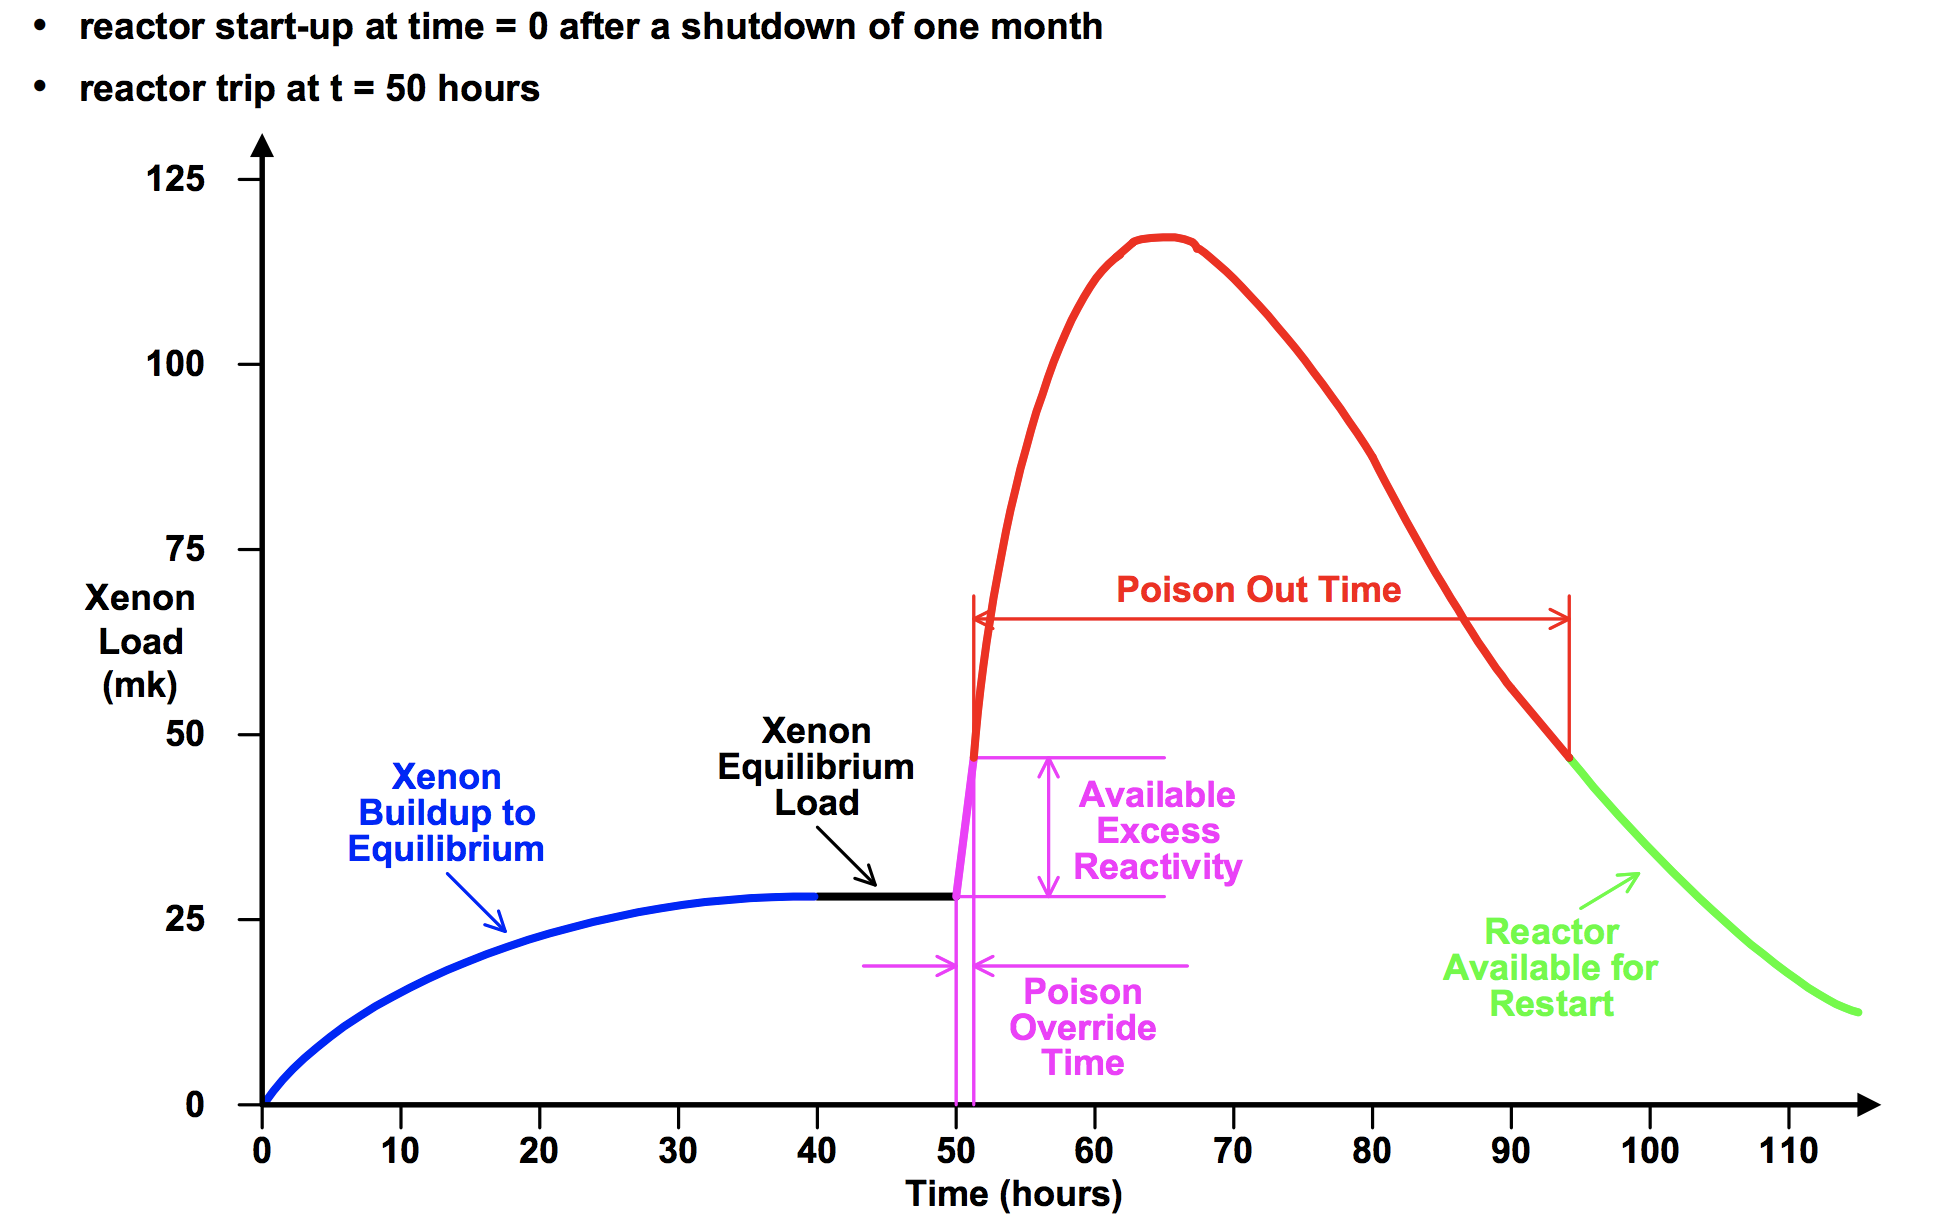
\includegraphics[width=\textwidth]{XenonPoison.png}
\caption{Xenon poisoning effect following shutdown from \parencite{garland2005}}
\label{fig:XenonPoison.png}
\end{figure}

Consequently, nuclear reactors aren't well suited to rapid fluctuations in power, particularly dramatic reductions in power, as these can lead to instability in the reactor core.  If the reactor is shut down in order to avoid such dangerous circumstances, it generally cannot be started again until Xenon levels have fallen again, which can take a couple of days.  Obviously this is never desirable for a military vessel, and hence is avoided at almost all costs.

This effect has a dramatic impact on nuclear submarine design, since much of their design is oriented around being able to comfortably disperse large amounts of excess power, rather than with conserving it.  For the propulsion system, this actually makes having an inefficient propulsor at low speeds a considerable advantage.  Since the reactor will likely need to dispose of excess power, particularly during ramp-down, an inefficient propulsion system actually provides a useful power sink.  Since any excess power will have to be disposed of by some other means (normally by pumping more water to remove the power as the heat) inefficiency at low speeds has no penalty, and probably a marginal benefit, since it will reduce overall demand for additional systems.    Provided the excess turbulence inside the pumpjet isn't too noisy, wasting energy through the propulsor is useful.

It should also be noted that a nuclear reactor's aversion to sudden reductions in power would also have a substantial impact on the design of a submarine's combat system, and it's demand on the Hotel Load. For the same reason, a high Hotel Load, or power-hungry Combat System, could actually be advantageous, as it helps to set an elevated 'floor' for power requirements, reducing the scale of fluctuations in overall power demand from the reactor due to changes in propulsion speed.

\section{Some essential concepts}

\subsection{Conservation of Energy}

This is perhaps one of the most fundamental and well-established principals in physics.  The essential idea is that energy can move or change in form, but it isn't ever created or destroyed.  Machines, plants and animals all derive their energy from a particular other source, which can be measured and evalutated to establish the limits of energy available.  Plants collect energy from sunlight falling on their leaves. Humans (as well as combustion engines) capture the chemical potential energy in organic matter, and release it by combining it with oxygen.  Hydro-electric power plants turn the gravitational potential energy of water stored at a height into electricity.

Conservation of energy has a particularly relevant embodiment in fluid flows, which is given it's primary expression in Bernoullis equation.  It says that the total energy in a connected body of fluid is constant, though it can change in form between kinetic energy (movement), gravitational potential energy (it being elevated) the heat energy in the fluid, and the pressure of the fluid.

In different fluids, the dynamics of how energy moves between one and another change.  For example, in gases, heating up a confined piece of gas will increase it's pressure, or if it is unconfined, increase its volume. This is particularly important for understanding gas turbines. In the case of a liquid, however, all the molecules are in close contact, and hence can't increase in volume or pressure substantially except by the creation of steam. As such, in the absence of large amounts of cavitation, the terms in the relationship which are most important for our consideration are the relationships between pressure, and kinetic energy, and gravity.

In the case of most waterjets which propel surface vessels, the water is lifted from the bottom of the hull at the intake to the pump, which is generally incorporated inside the hull. This increase in gravitational potential coincides with a slowing down of the water relative to the vessel-speed. Since the jet in such vessels is generally ejected at the same height as the pump, this potential is never regained, and is technically a loss, however at high speeds such a loss is small relative to the total power ouput.

\subsubsection{Venturi Effect}
In the case of submarines and torpedoes the water doesn't undertake a change in height, since intake and nozzle are generally all in line with the central axis of the submarine or torpedo.  As a consequence, the key relationship in Bernoullis equations is the relationship between the liquids velocity, and its pressure.  The consequence is that when water moves through a pipe (duct, or shroud) it's pressure is inversely related to the square of its velocity.  This means that when a liquid is forced to to travel through a narrowing pipe, it's pressure necessarily decreases as the velocity increases.  This is a simple embodiment of the Venturi effect.

\subsubsection{Flow Diffusion}
The inverse process is where a pipe increases in volume, and the flow is forced to slow down in order to fill the wider area, and the pressure correspondingly increases.  This is a process called 'diffusion', and is important to achieving high pressure levels in many types of water pumps, including those which will be particularly relevant for pumpjets for watercraft propulsion \parencite{hamilton1997}.

\subsubsection{Energy waste and efficiency}
The conservation of energy also has useful implications for how the efficiency of systems is thought about.  In particular, because energy is conserved, identifying inefficiencies in a system necessarily involves identifying where energy goes to doing tasks which aren't useful for the intended purpose.  A perfectly efficient system won't do any work that isn't for the intended purpose.  In the case of analysing the efficiency of propulsion systems, the relevant 'work' is almost always related to moving water backwards to produce thrust.  Moving water in directions other than backwards, including random turbulent flows which wind producing heat rather than thust, are two examples of wasted energy.  Noise in the water also reflects energy which is wasted.

\subsection{Boundary Layer}
When water or any fluid flows with some speed relative to another solid surface nearby, there is some layer adjacent to the surface in which the speed of the fluid is diminished relative to the main flow.  At a microscopic level, there are some molecules of the fluid on the surface which will be effectively static relative to the surface.  The layer of fluid that joins the gap between the static surface, and the part of the flow which is moving at the full flow speed, is called the boundary layer.  Exactly how thick the boundary layer is, and how the fluid moves in the boundary layer, is extremely important for consideration of efficiency of fluid flows over and around solid surfaces.  In particular, a boundary layer can be either turbulent or laminar in nature, and can transition to turbulent flow after a short distnace of laminar flow, as shown in Figure \ref{fig:BoundaryLayer.png}.


\begin{figure}
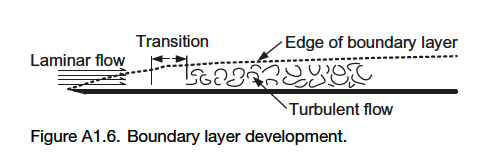
\includegraphics[width=\textwidth]{BoundaryLayer.png}
\caption{The development of a boundary layer as shown in \parencite{mollard2011}}
\label{fig:BoundaryLayer.png}
\end{figure}

\subsection{Turbulent and Laminar Flow}
The way that fluids move relative to a surface can one of either two methods.  In 'laminar flow' all the fluid moves in one direction in an smooth and orderly manner, with very little mixing between the layers of fluid travelling at different speeds.

The alternative is 'turbulent flow', where the fluid moves around in unpredictable swirls and circles as well as moving overall in an predominant direction.  There is considerable mixing between all the different layers, and the average speed remains relatively constant in the flow, with the exception of the flow immediately adjacent to the wall, or in the boundary layer.  Becuase turbulence involves a lot of movement that is not overall in one productive direction and contributing to thrust, it necessarily leads to some loss of energy from the overall thrust.  Once the swirls and movements become smaller and smaller, the energy winds up simply as heat in the fluid.

\begin{figure}
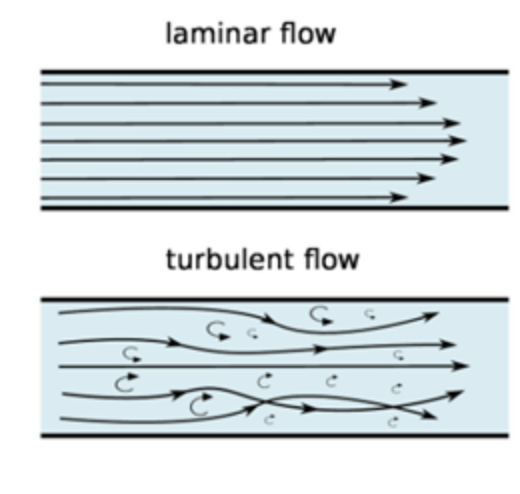
\includegraphics[width=\textwidth]{LaminarTurbulent.png}
\caption{A simple comparison of laminar and turbulent flows from \parencite{NPdotnet2017}}
\label{fig:LaminarTurbulent.png}
\end{figure}

The likely point of transition between a flow being turbulent and laminar can be given by unitless number called the Reynolds Number, which is determined by a fluids velocity, viscoscity, density, and a characteristic length-scale over which the flow occurring.  A fuller discussion of these important concepts can be found in \cite{NPdotnet2017}.

Turbulent flows in gasses can be extremely noisy, since those fluids are compressible.  Consequently, the rapid and intense ciruclar movements result in a lot of oscillatory compressions against the surrounding air.  Consequently things like jet engines, vacuum cleaners, hand-dryers, and other devices that create rapid movements in gasses tend to be quite loud, including at some distance.

In essentially incompressible fluids, the random changes in pressure and velocity which are involved in laminar flow tend not to generate nearly as much noise in the surrounding liquid outside the flow.  Because the fluid is incompressible, all of the random 'round and round' movements don't amount to much 'in and out' movement, which is what creates the pressure waves which result in propagated noise. Consequently, whilst turbulent flows do inevitably generate some noise, the amount of noise generated is dramatically greater in the presence of cavitation, where a void opens up in the water, and vastly more 'in and out' movement is able to occur.

\subsection{Cavitation}
Cavitation is the rapid expansion and collapse of a void, or bubble in water. Put technically, caviation occurs when the local static pressure (pressure in the rest frame of the fluid) falls below the vapour pressure of the fluid (pressure at which the liquid will start to boil).

Imagine what happens when something moves very fast through water.  The front side of the object pushes the water forward, but on the back side the water has to push in to fill the space left behind.  If there’s not enough pressure to push the solid water in fast enough, a gap opens up, with just a few gaseous water molecules (steam) inside the cavity.  (This is also described as water boiling at low pressure.)  However the gap doesn’t stay around for long.  Soon the water catches up, and the bubble implodes with a pop, leaving only tiny bubbles as a result, which you can see in the wake of almost any boat or ship moving at speed.  Whilst some energy turns to heat (the remaining steam in the tiny bubbles) quite a bit is propagated away as a sound-wave generated by the implosion.

A watching water boil in a glass kettle gives a quick and intuitive insight into the occurrence of cavitation.  Quickly after the kettle starts heating, a considerable noise can be heard, which corresponds to the commencement of cavitation on heating element. At some local point for a moment in time, there is enough energy for the water present to boil.  It tends to be on rough surfaces or in the presence of some impurity that cavitation will occur first (in the blackened part of the surface in this case.)  However, whilst the bubbles on the bottom can be seen plainly on the bottom, they collapse almost straight away again, and leave only a tiny bubble of stable steam ciculating in the water.  It is the rapid expansion and collapse of these bubbles that causes the noise of a kettle, long before it has boiled.

\begin{figure}
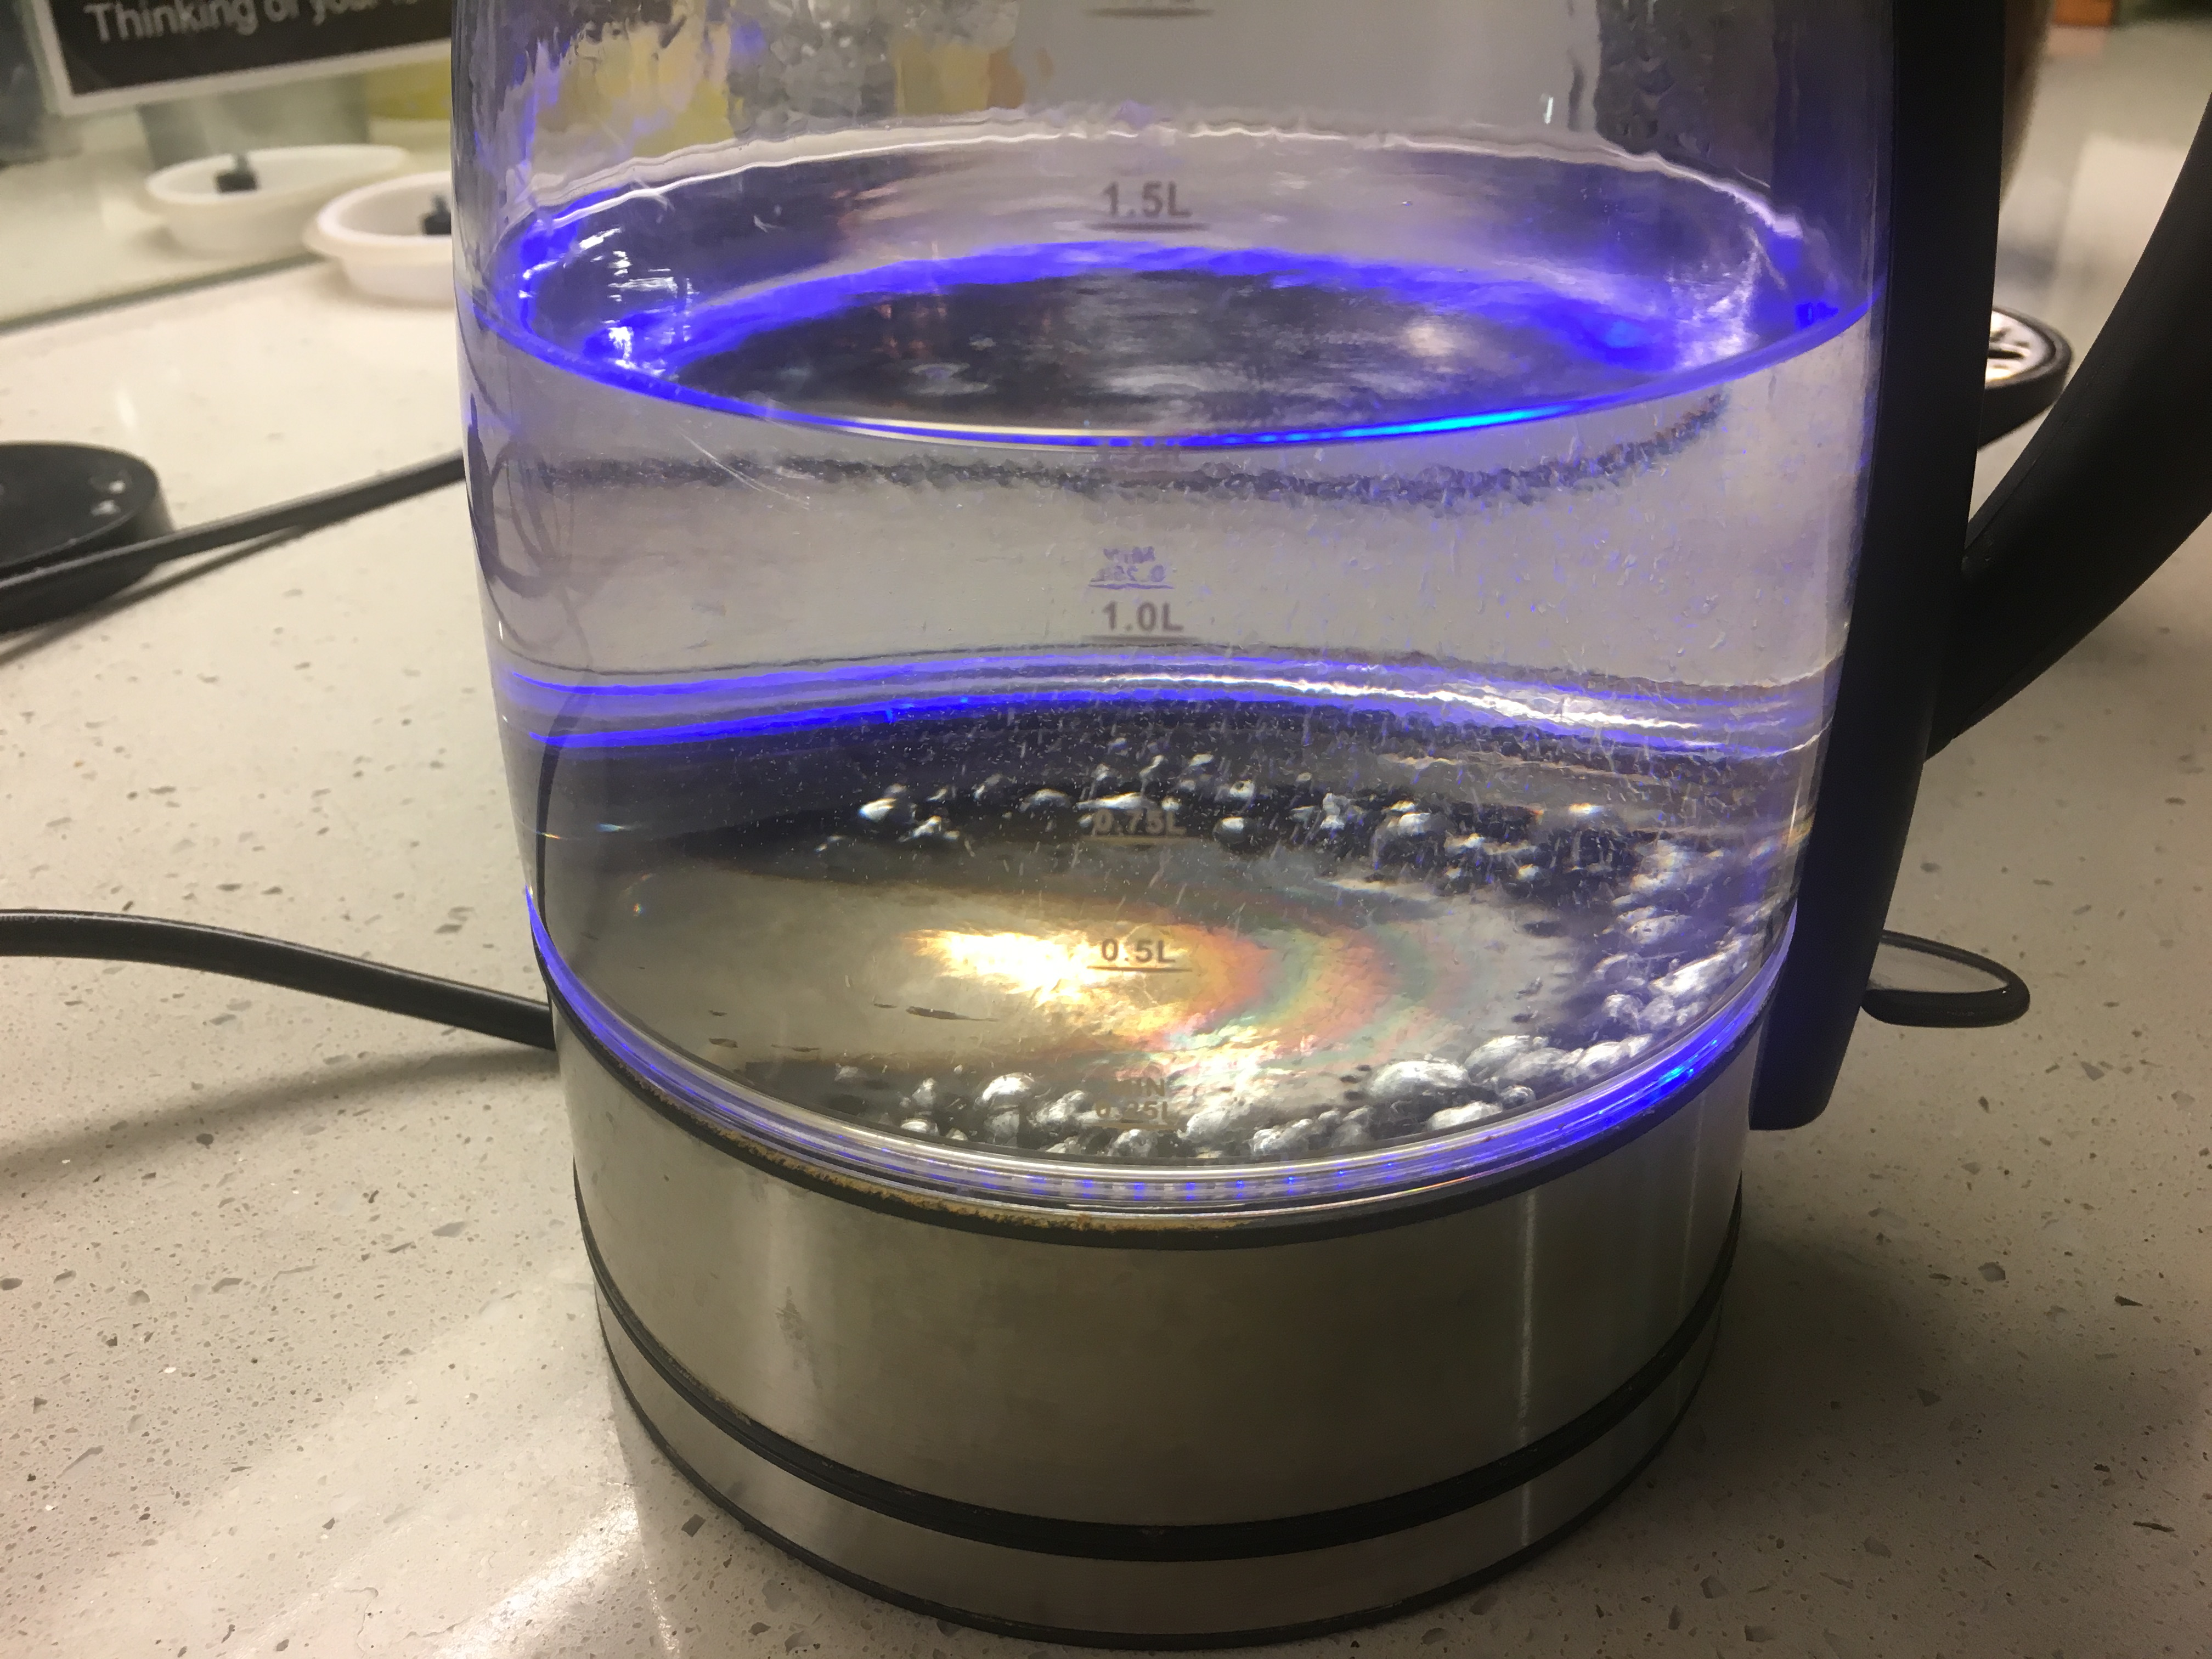
\includegraphics[width=\textwidth]{EarlyCavitation.JPG}
\caption{Cavitation bubbles form and collapse creating noise and some tiny bubbles long before boiling occurs}
\label{fig:EarlyCavitation.JPG}
\end{figure}

It is only when the water is all at a much higher temperature that the bubbles remain their full size for long enough to detatch and rise all the way to the surface, a process we typically think of as boiling water.  It is worthwhile noting that the sound emitted at this stage is much softer and lower than the early onset of cavitation. Larger bubbles result in lower frequencies of sound being emitted. Even at higher temperature, the rougher parts of the surface provide the points where all the cavitation originate.

\begin{figure}
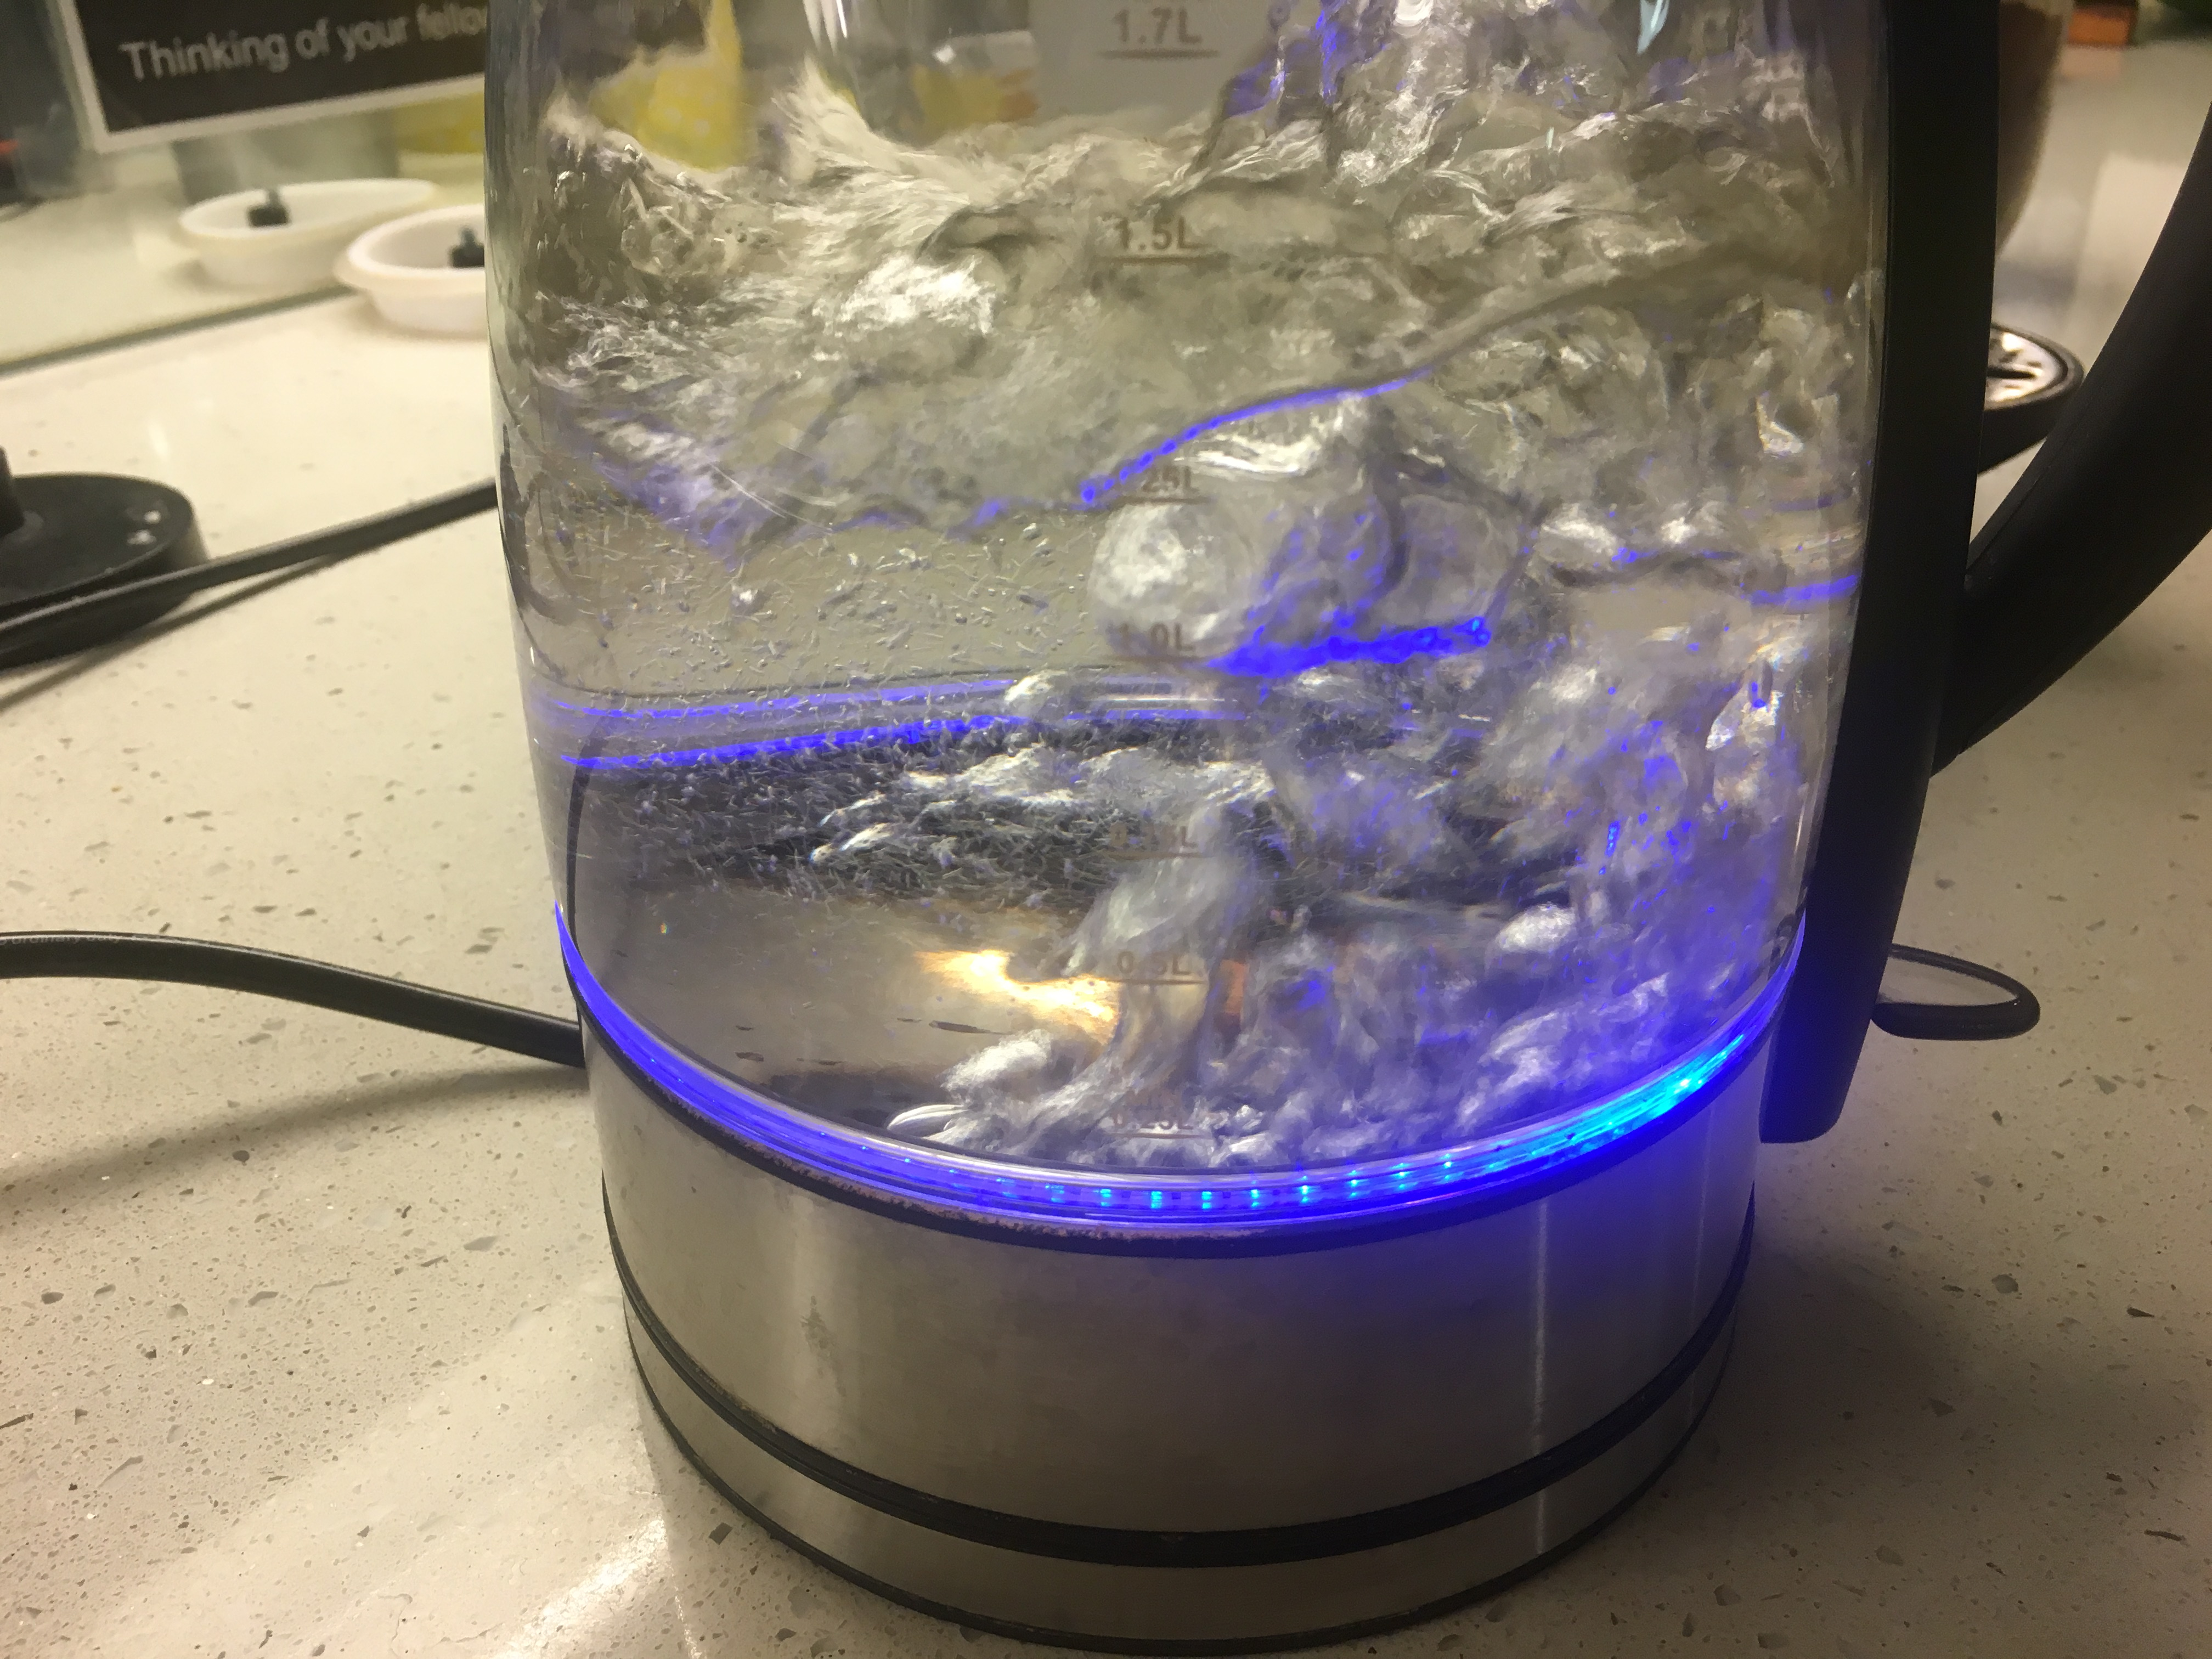
\includegraphics[width=\textwidth]{BoilingCavitation.JPG}
\caption{Only at very high temperatures do the bubbles endure at full-size in the water and reach the surface}
\label{fig:BoilingCavitation.JPG}
\end{figure}

Cavitation is extremely important in the study of ship propulsion, since it's occurrence in particular circumstances can lead to substantial losses of efficiency, as well as damage to the propeller and related appendages. It is particularly important for submarines, since the expansion and collapse of these bubbles tends to lead to the creation of noise which is often far larger, and more distincly characteristic than other turbulent disturbences in the water when no cavitation is present.  Consequently, the onset of cavitation can be thought of as a distinct threshold in terms of the acoustic performance of propulsive system.

Despite cavitation necessarily representing some energy being wasted generating unwanted noise in the water, some cavitation inevitably occurs around most propulsion systems operating at full power.  In plenty of cases, the consequences for efficiency are relatively small, as they tend to be dominated by other efficiency considerations in imparting thrust.  Put another way, the savings that can be gained by minimising wastage to turblence can outweigh the losses incurred by having some cavitation occur.  In most cases, propellers are designed to work with a certain extent of cavitation for optimum efficiency under working loads \parencite{shin2015}. Cavitation also occurs to a considerable extent within the jets of most high-speed surface vessels, but doesn't necessarily have a particularly bad effect on their overall efficiency at their intended speed levels.  It is generally only within very specialised military circumstances when the absolute avoidance of cavitation supercedes other concerns for efficiency, and require the elimination of all cavitation entirely \parencite{mollard2011}, \parencite{lewis1988}.  These circumstances include the design of submarines and torpedoes.

In certain special cases, particularly supercavitating propellers or surface-piercing drives, high levels of cavitation can be higly advantageous for efficiency.  However these represent specialised designs, generally only for very high speed vessels, where acoustic concerns are negligible, and are of little concern for this particular endeavour.

Cavitation can occur in a number of different ways at different points and forms on or around the propeller.  It is common for cavitation to occur first near the out extremities of the propeller, where the blades are moving at the highest velocity relative to the water-flow.  Cavitation tends to spread across the back of the blades in a sheet (sheet cavitation), since the back side of the blades are generally the areas of most depressed pressure, though it can also occur in places on the back side of the blades, where the dynamics of the water moving around the blade can produce points of near the edges of significantly reduced pressure.   On surface vessels cavitation tends to occur most when the blades are closes to the surface, where the pressure is lowest.

\begin{figure}
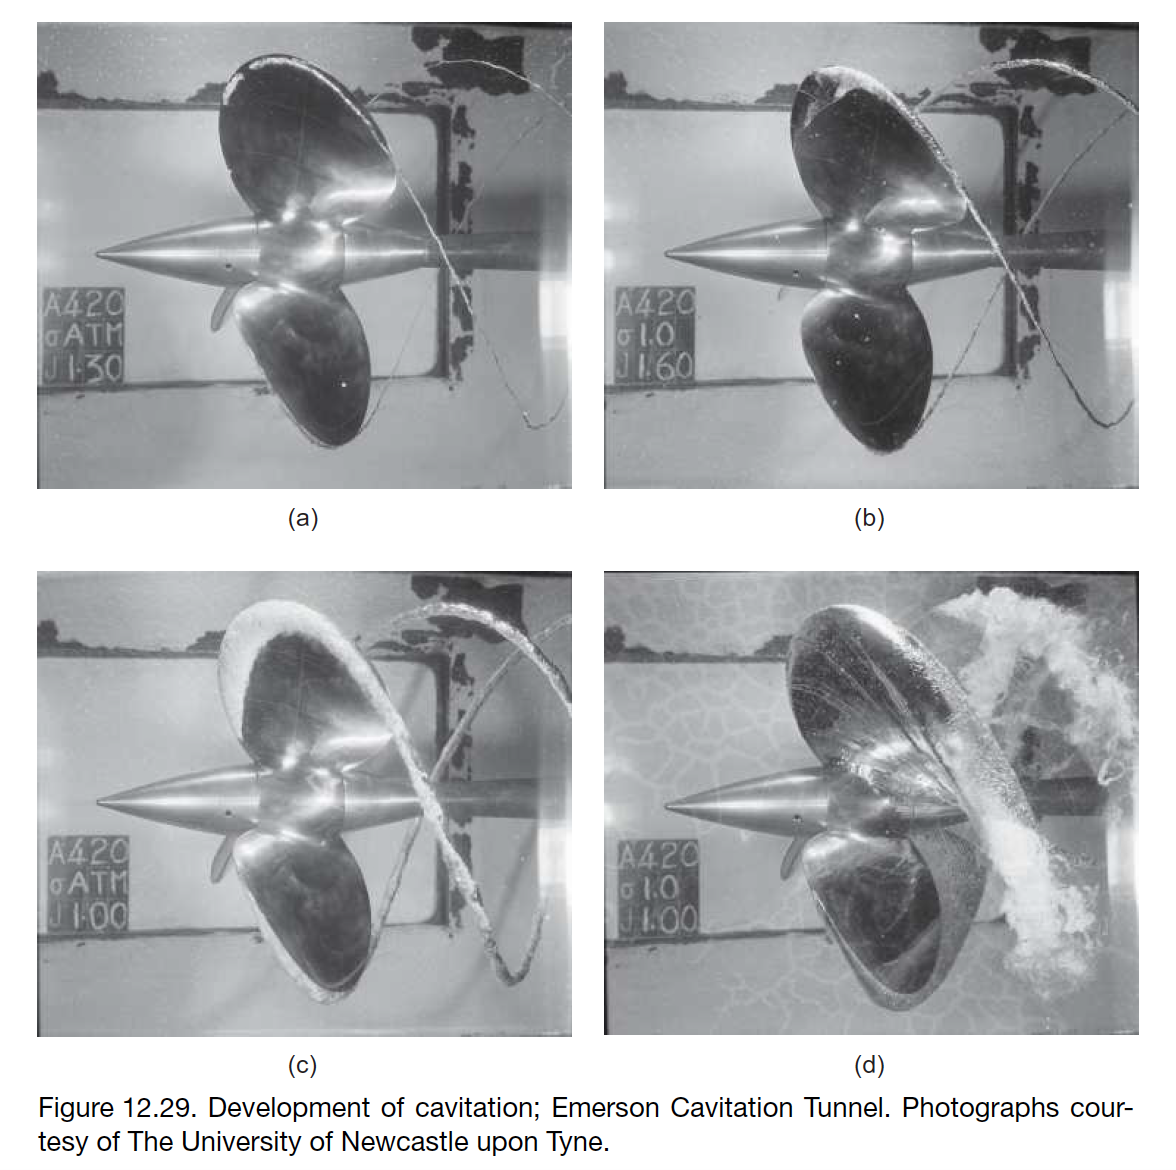
\includegraphics[width=0.7\textwidth]{IncreasingCavitation.png}
\caption{Cavitation frequently occurs first at the extremities, then spreads inwards across the blad face, as shown in \parencite{mollard2011}}
\label{fig:IncreasingCavitation.png}
\end{figure}

\begin{figure}
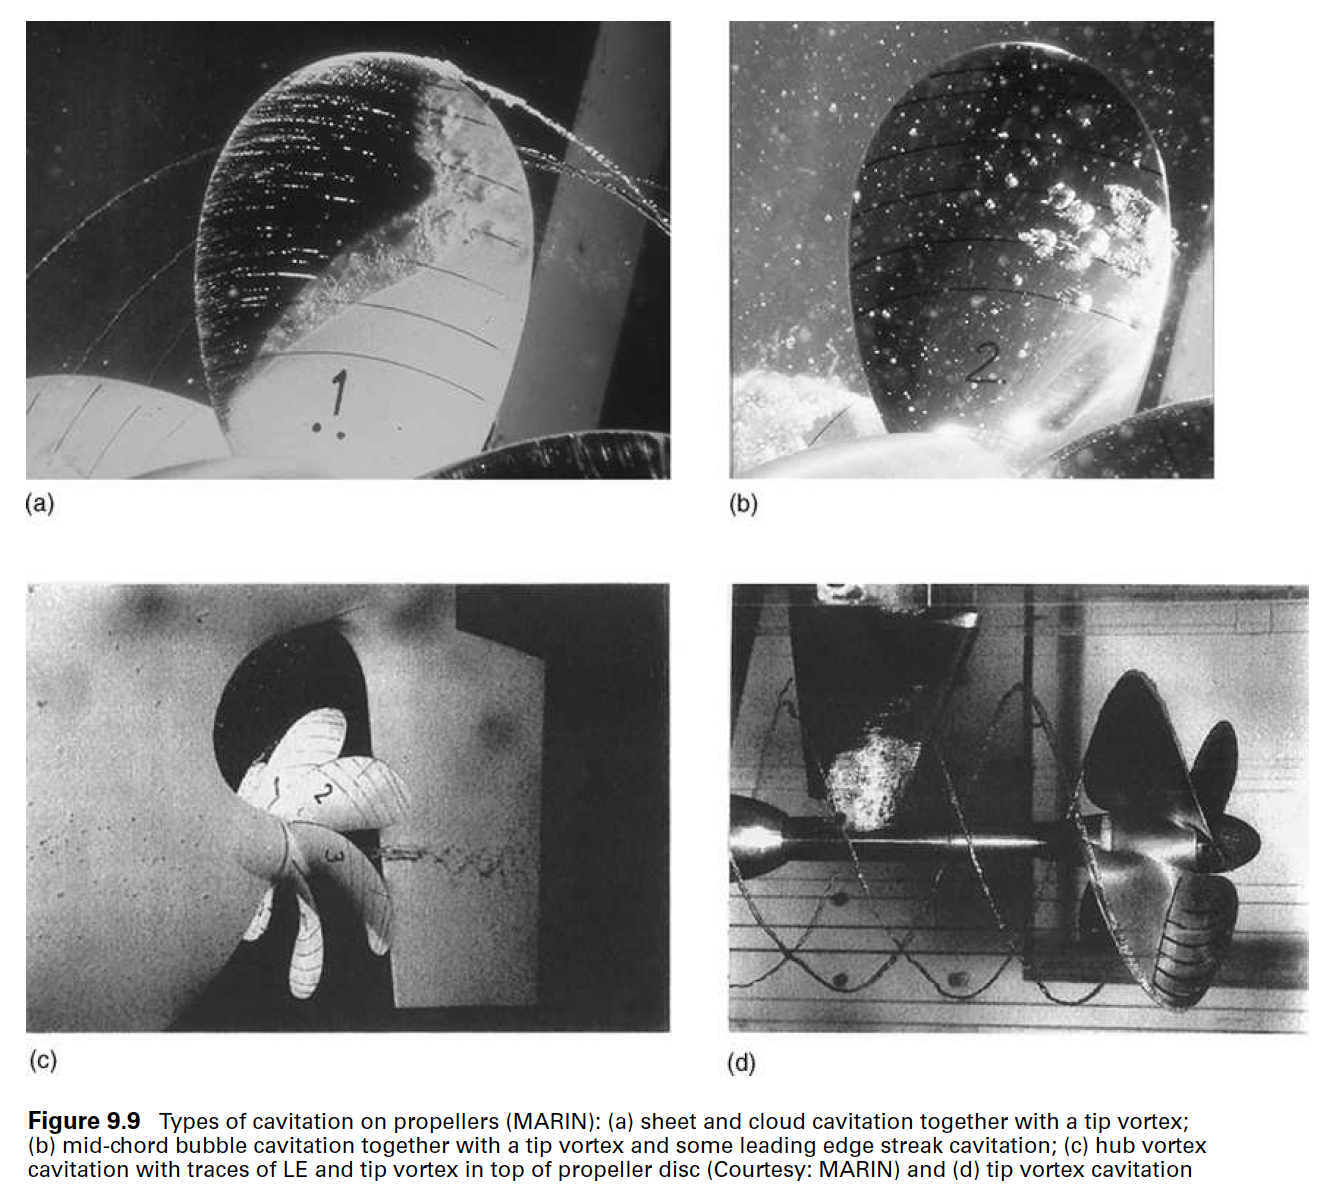
\includegraphics[width=0.7\textwidth]{CavitationTypes.png}
\caption{Different types of cavitation can occur on different parts of the propulsion system as shown in \parencite{carlton2007}}
\label{fig:CavitationTypes.png}
\end{figure}


\subsection{Pressure, Thrust, and Momentum change}
It is worthwhile spending just a moment to touch on the relationship between a few different concepts which are closely related.  Thrust is a force, measured in Newtons, which is generally used to refer to the forces acting on a vessel or object by its propulsion system to move it forward in the water.  Generating thrust is consequently a key objective of any propulsion system.

Pressure is a measure of force divided by an area over which it is applied. Pressures are necessarily applied to some extent over all of the surfaces of any object, including due to the atmostpheric pressure of air.  In considering the efficiency of propulsion systems for solid bodies, thrust is always the consequence of some \textbf{net} pressure difference on different sides of an object.  For instance, on a propeller blade, the rear-facing side of the blade is the side that pushes the water backwards, and hence has a raised pressure on its surface.  Being generally backwards facing this acts to push the propeller forwards.  This pressure acts equally to push water backwards, as well as to push the propeller forwards.  Importantly, the forward-facing side of the propeller will expereince a lowered pressure, which also serves to pull water backwards, and suck the propeller forwards.  It is the sum of all the pressure differences on the propeller that result in a net force.

Importantly in hydrodynamics, it is important to consider the possibility of other forces being generated other surfaces which may have an impact on the movement of the vessel.  In the presence of the hull, water being drawn by the propeller can cause pressure changes on other surface of the vessel which may assist or impede producing a net positive thrust.  Submerged jets represent a particular case in point.  A famous home experiment suggests that one compare the thrust (backwards pressure) experienced by someone holding a garden hose creating a jet of water when it is in the air, as opposed to submerged in a pool of water.  When submerged, the backwards pressue appears dramatically reduced.  In fact, this phenomenon is due to a the water-jet drawing adjacent water with it under-water, the movement of which exerts a negative pressure on the outside of the nozzle, conteracting the pressure exerted on the inside of the nozzle. This effect represents one of the important distinctions between the jets which release their water below or above the water-line.

It is also an important law of physics that force or thrust is equal to the rate of change of momentum. Put simply, the speed at which one speeds something up, or the increasing amount of something which begins to move, is always equivalent in magnitude to the thrust that is produced.  Since momentum is a vector, this simple law requires that the momentum change has to net out to one particular direction in order to produce a net thrust.  Circular movements necessarily are cancelling, and produce no thrust. It is useful to recall however that this principal is simply another complete and way of measuring the consequences of the net pressure differences discussed earlier.  The total rate of change of momentum in the water-column which is induced as a conseqence of the pressure differentials on all sides of the propeller must necessarily be equivalent to the total net force that is produced.  Consequently literature seeking to optimise propulsion might discuss analysis referring to both of these effects or phenomena, and neither are in conflict.

Full and proper derivations of many of the thrust equations for different propulsion systems from these principals can be found in plenty of authoritative works, including \cite{lewis1988}, \cite{carlton2007} and \cite{mollard2011}.

\subsection{Flow separation}
Flow separation refers to a circumstance when the flow over a surface separates entirely from the surface, and a new eddy or votex is formed where the flow actually moves in the opposite direction to the dominant flow.  It is of particular significance in hydrodynamics because it can lead to substantial losses of efficiency, as energy is diverted into the kinetic energy of the eddy or vortex, which is unproductive. It tends to occur near the surface of aerofoils with high angles of attack, or in the blades of turbomachinery including diffuser or mixed-flow pumps and ducted propellers operating in off-design conditions, including low flow rates \parencite{li2013}, parencite{bakker2006}, parencite{mcbride1979}, parencite{wislicenus1986}.

\begin{figure}
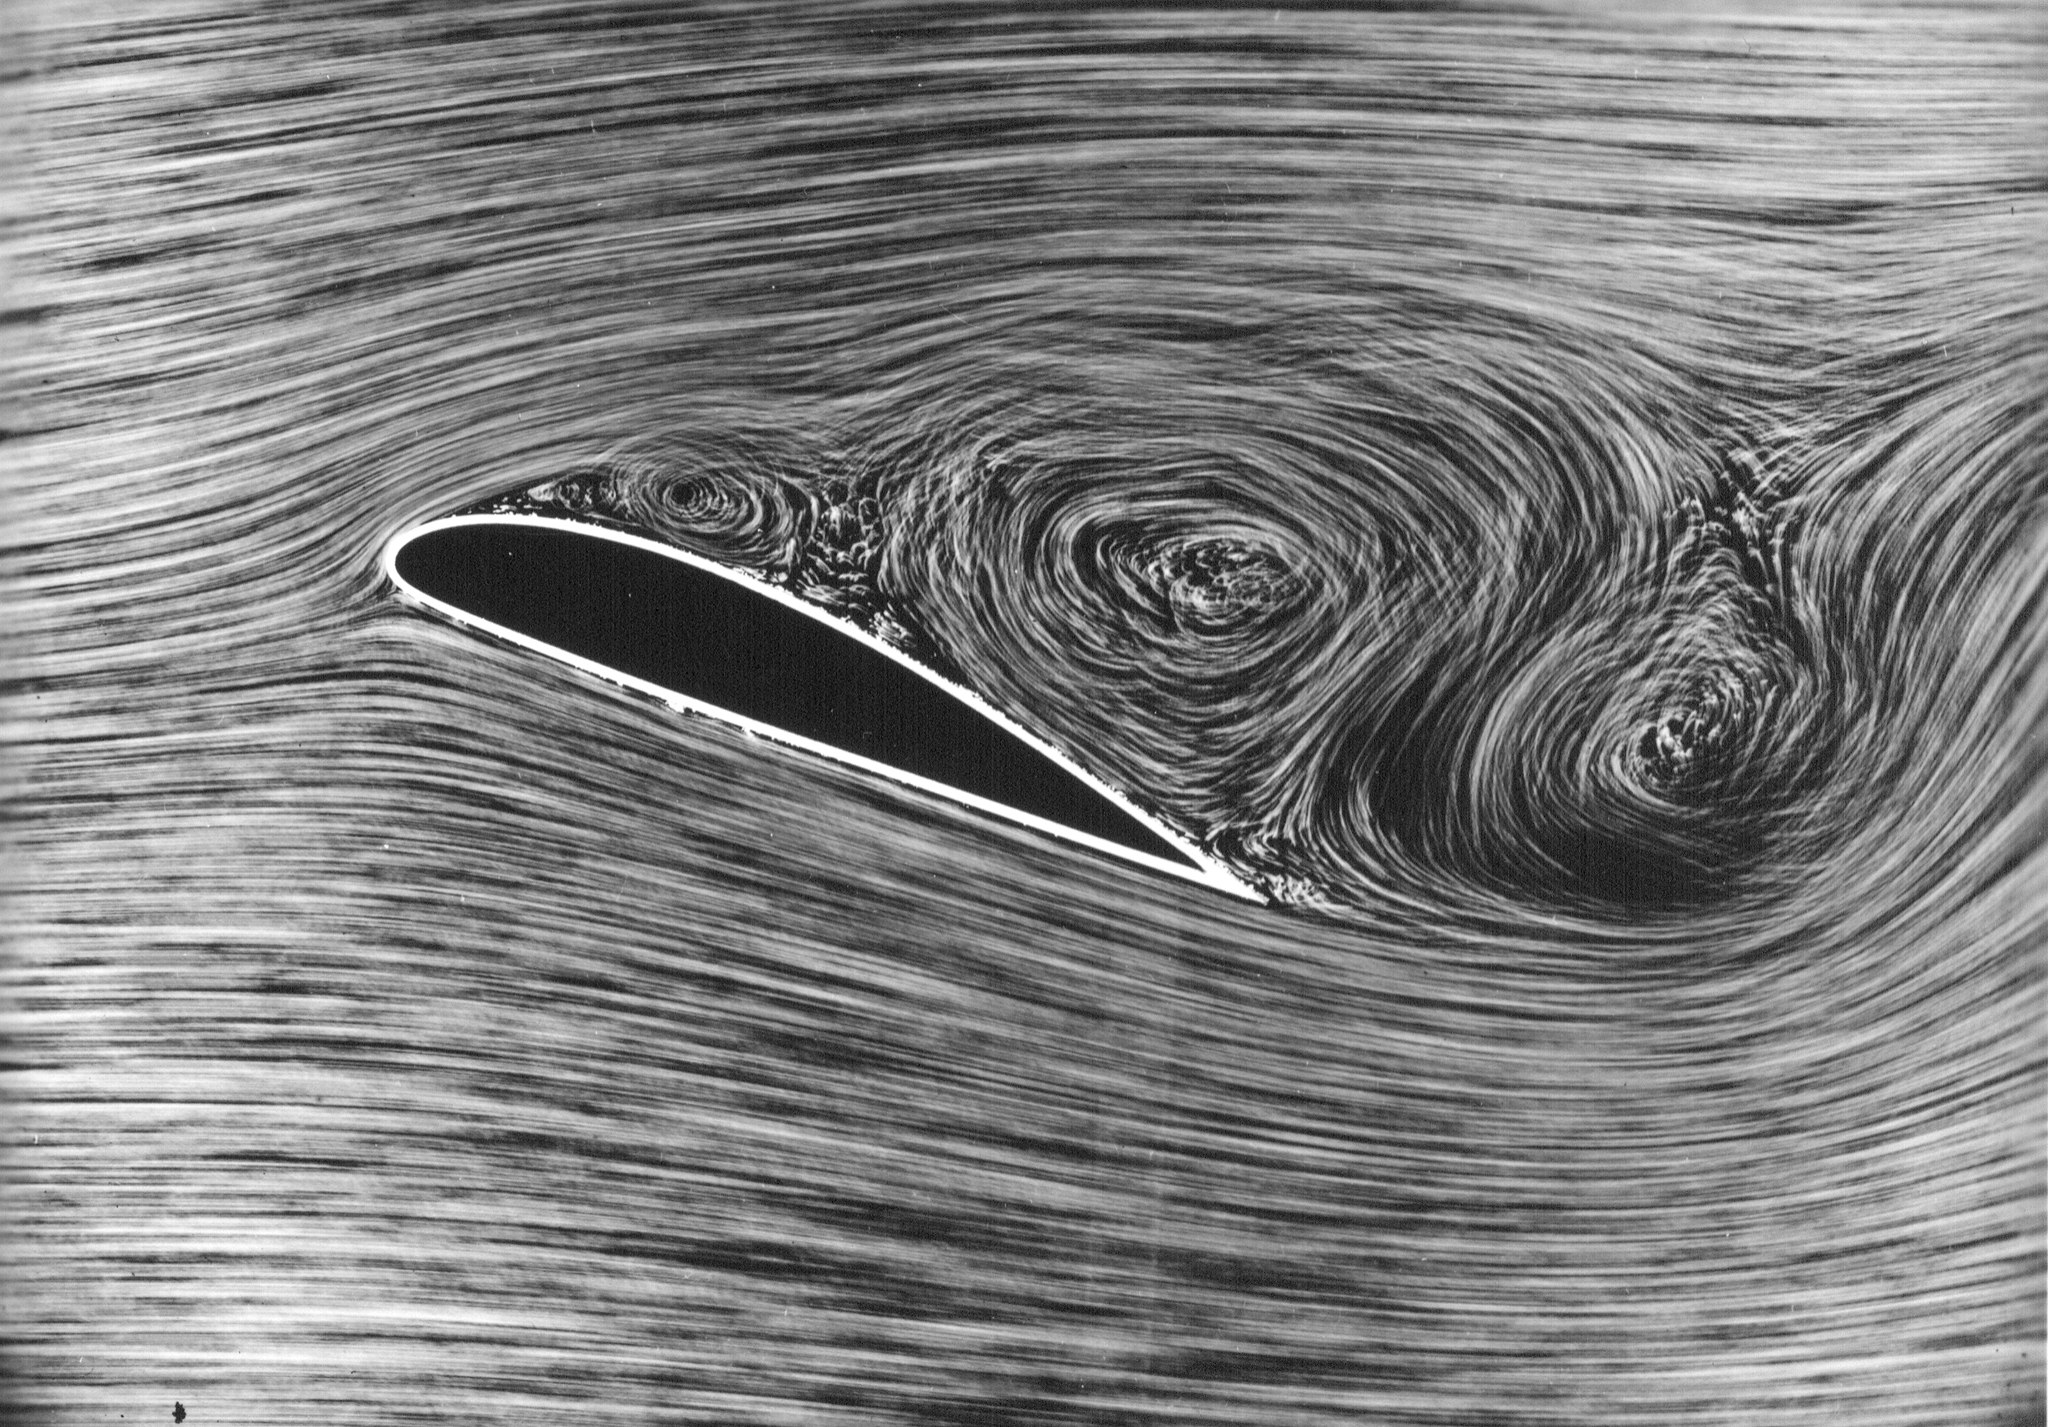
\includegraphics[width=0.5\textwidth]{SeparatedAerofoil.jpg}
\caption{Flow separation occurring over the top of an aerofoil in a wind tunnel. Image courtesy of Deutsches Zentrum fuer Luft- und Raumfahrt e. V. (DLR)}
\label{fig:SeparatedAerofoil.jpg}
\end{figure}

In order for flow separation to occur, a fluid must be moving against an adverse pressure gradient, which simply means that the pressure is increasing in the direction of movement, which means the flow is slowing down as it moves.  At the boundary layer, where the flow velocity is already reduced due to drag forces experienced near the surface, the adverse pressure gradient can be enough to reverse the flow altogether.  In this case, the fluid flows in reverse near the surface and forms a vortex, and the main flow becomes separated form the surface by the votex.

\begin{figure}
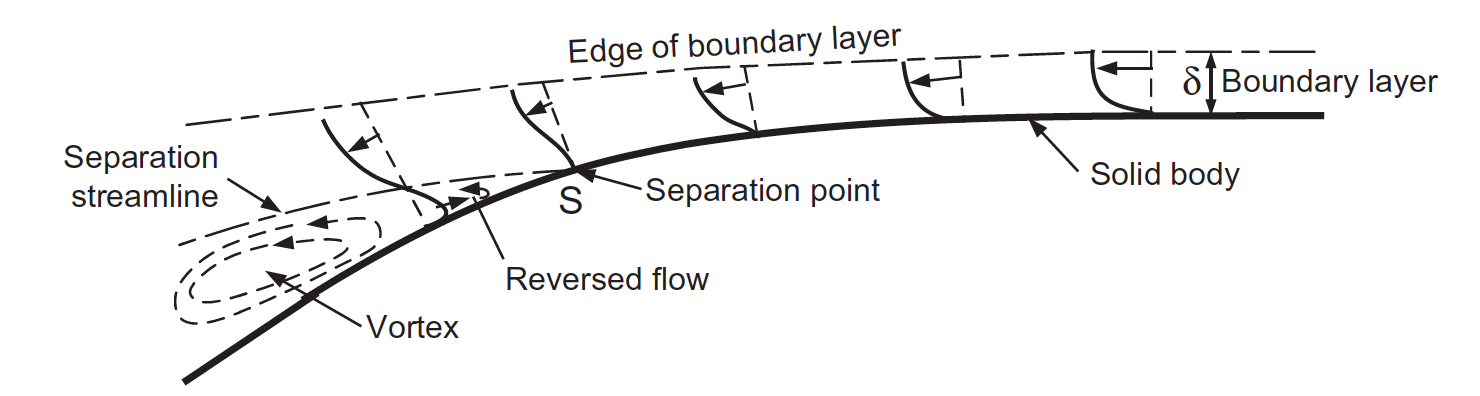
\includegraphics[width=\textwidth]{FlowSeparation.png}
\caption{Flow separation involves flow reversal near a surface when a fluid is moving against an adverse pressure gradient, as shown in \parencite{mollard2011}}
\label{fig:FlowSeparation.png}
\end{figure}

In addition to the necessary loss of efficiency, flow separation can often tend to result in unsteady flows, with the vortices periodically being shed into the flow \parencite[480]{mollard2011}.  If this occurs ahead of the blades of a propeller or impeller, such disturbances to the flow can lead to instances of cavitation when otherwise a steady homogenous flow might be well below the cavitation inception point, and can be consequential for the acoustic performance of the system, particulaly if such shedding resonates with characteristic frequencies of any of the machinery.

\section{Basics of Ducted Propellers and Pumpjets}
It's easy to be somewhat confused by the many different names which seem to be associated with related, or similar systems.  Between pumps, pumpjets, water-jets ducted or shrouded propellers, or impellers, there is plenty of grounds for some confusion  In this section, I aim to clarify in simple terms what the important differences between distinctly different systems are, and where some terms are used somewhat interchangeably without doing any great violence to the concepts underlying.

\subsection{Propellers}
Perhaps the best starting point is the most basic, and oldest of the systems which we're considering: the basic screw propeller.  A propeller uses a number of tilted blades attached to a central hub to sweep around disc in the water, and accelerate a column of water passing through the disc.  Due to the slant of the blades, water on the back sides of the blades is pushed astern, and reduced pressure on the front faces pulls more water from ahead to replace it.  As such, it accelerates a column of water, which necessarily is contracted in circumference after the point of acceleration.

\begin{figure}
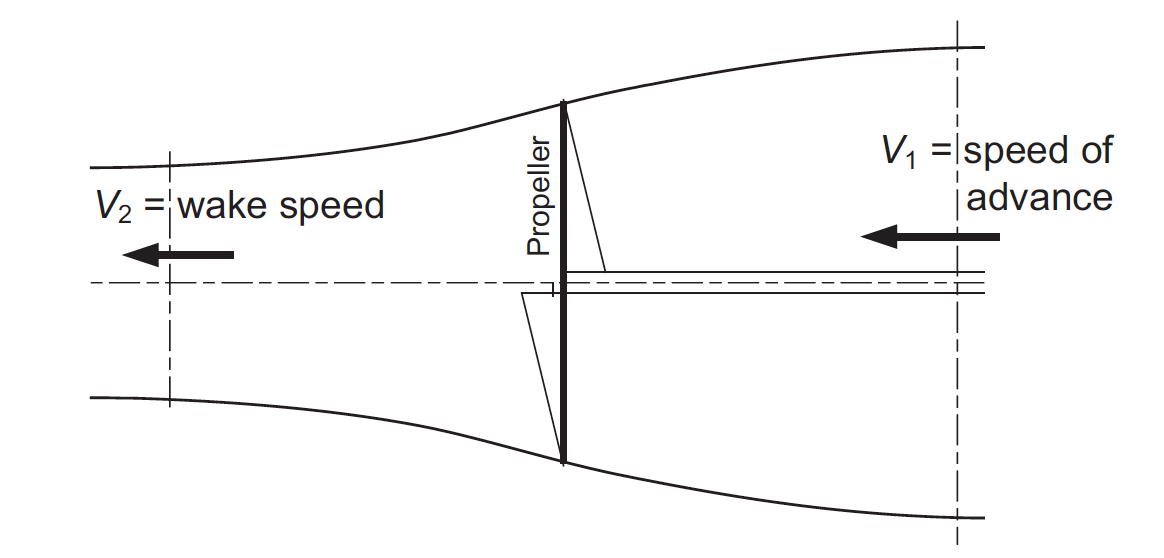
\includegraphics[width=\textwidth]{PropellerAction.png}
\caption{Propellers generate thrust by accelerating a column of water, as shown in  \parencite[247]{mollard2011}}
\label{fig:PropellerAction.png}
\end{figure}


A comprehensive description of the development of the propeller can be found in \cite{carlton2007}.  Here I won't elaborate on beyond describing some essential features and characteristics with which one ought to be familiar, primarily for the purpose of comparing different propellers and their evolution into impellers of different designs.

Most propellers will have between three and seven blades.  In general they are shaped as an aerofoil, with the convex side being upstream, just as the convex side of a plane wing is above, in order to generate lower pressure and lift as it moves through the air.  The blades tend to be twised so that they have a higher angle of attack closer to the hub, and lesser closer to the extremities, so that those faster moving sections push their respective parts of the water column at an overall similar speed.  The are often also thinner towards the extremities, and will be swept backwards as if dragged by their rotation through the water (skew) and also dragged by the ship's movement throug the water (rake). Whilst the degree of all these characteristics is highly variable for different applications, these are a few of the commonly referred to characteristics which can be varied in order to optimise performance for any given application.

\begin{figure}
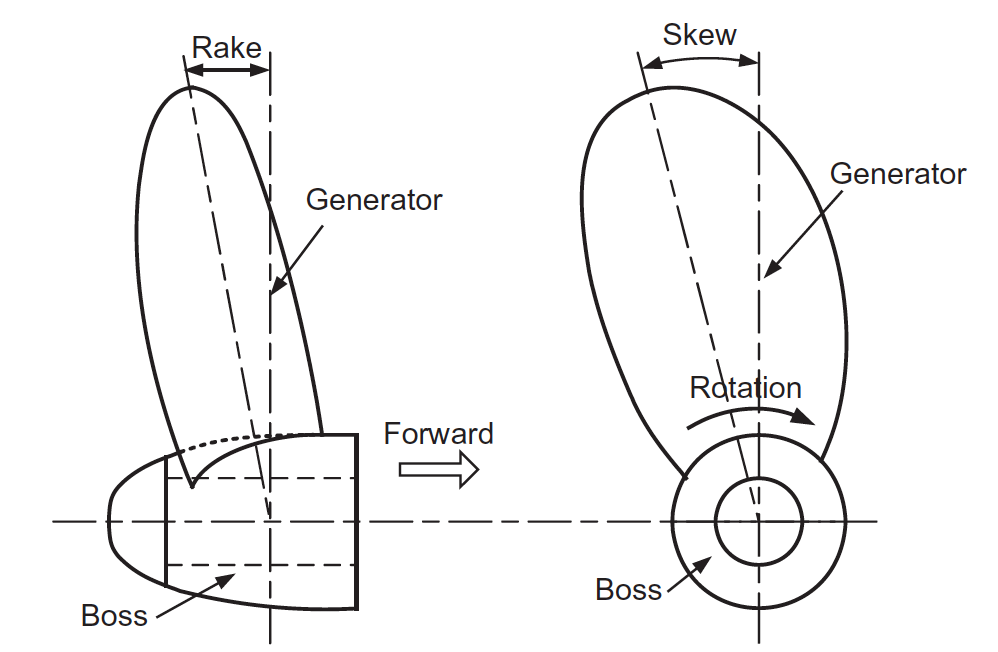
\includegraphics[width=\textwidth]{SkewRake.png}
\caption{The development of a boundary layer \parencite[262]{mollard2011}}
\label{fig:SkewRake.png}
\end{figure}

\subsubsection{Pitch}
Perhaps one of the most important characteristics of a propeller is its pitch.  The pitch represents the distance that a blade section would travel forward if it carved its way around a helix through one full rotation.  It is intuitive to think of as something akin to the angle-of-attack of the propeller blade to the water, however this is technically misleading as the movement of the water-column incoming to the blade, as well as the speed of rotation, also have a significant bearing on what the actual angle of attack of the blade ends up being.  Whilst technically pitch is a distance (measured in meters), it is often expressed and used in formula as a ratio of the diameter of the propeller, to give it a unitless equivalent, as is common in the description of propellers and propulsion systems.

\begin{figure}
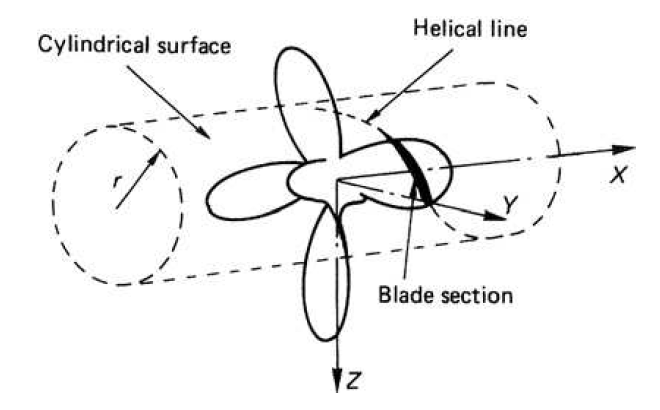
\includegraphics[width=\textwidth]{HelicalLine.png}
\caption{A blade section of a propeller traces a helical line around a cylinder as it is rotated \parencite{carlton2007}}
\label{fig:HelicalLine.png}
\end{figure}

\begin{figure}
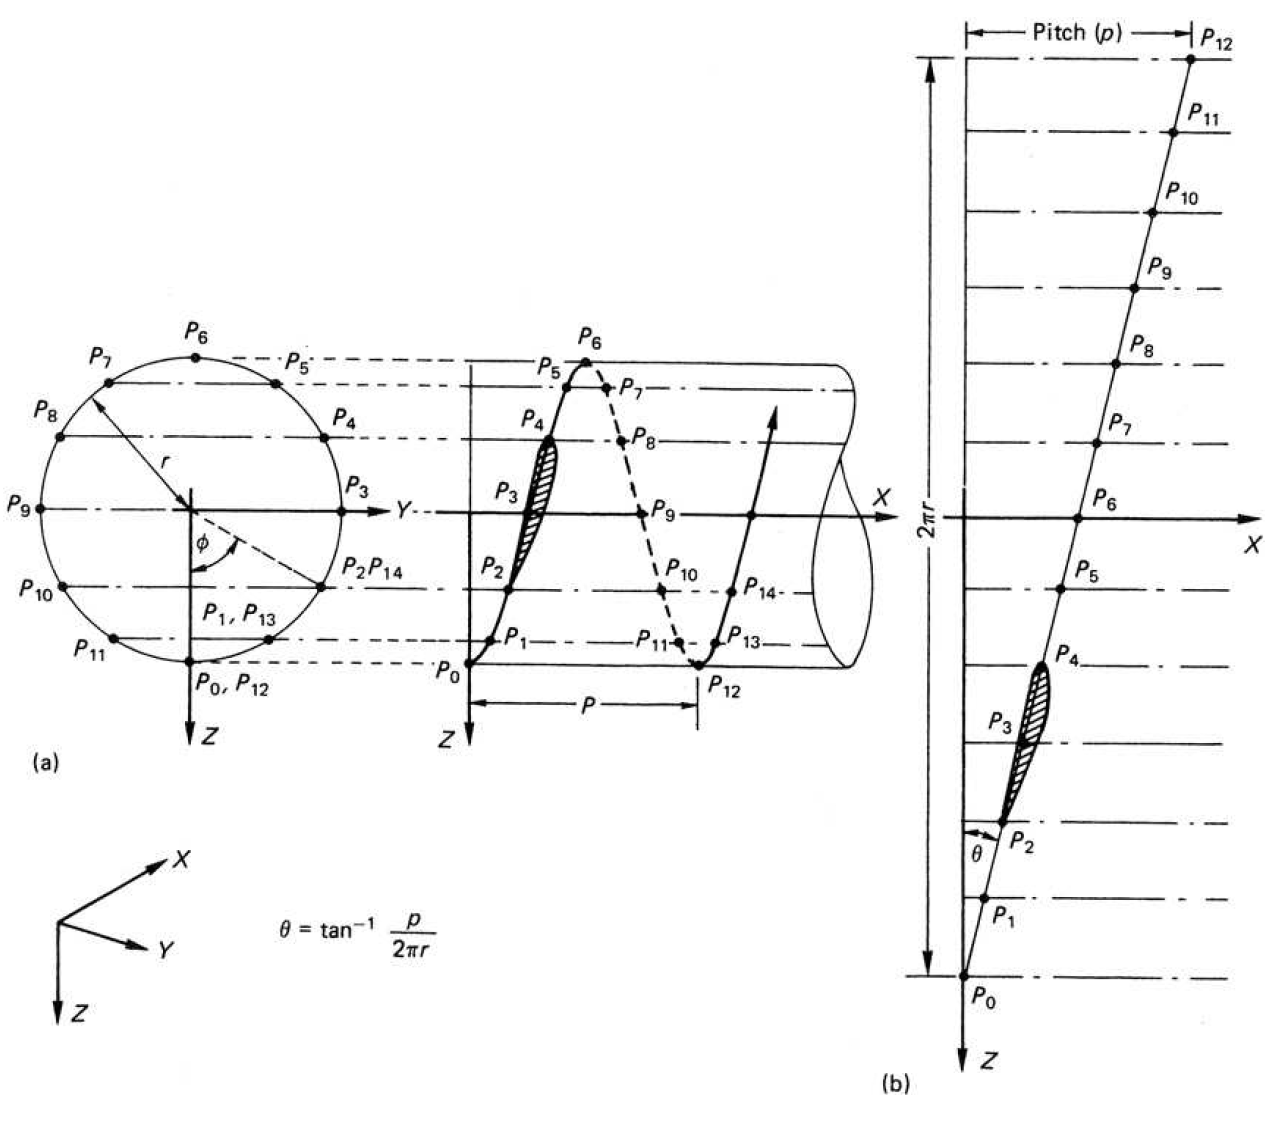
\includegraphics[width=\textwidth]{PitchDefinition.png}
\caption{The definition of pitch is the distance traveled by a blade section along a cylinder, as given in \parencite{carlton2007}}
\label{fig:PitchDefinition.png}
\end{figure}

The selection of the exact blade selection that is selected to define pitch must be specified as being at some fraction of the radius from the centre.  This distance is calculated to be the 'moment mean' or a technical derived effective average, which tends to lie between 0.6R and 0.7R.  A thorough discussion of pitch can be found in \cite[35-37]{carlton2007}.

Pitch is of particular importance to the discussion the efficiency of propeller and propulsor design because its optimal choice tends to vary considerably with the different loads which a vessel is intended to operate at, which can also relate to a vessel's design speed.  It is for this reason that a considerable number of vessels actually have variable pitch propellers.  Whilst considerably more complex, expensive, and heavier than a traditional fixed-pitch propeller, the ability to vary the pitch of a propeller assists considerably, particularly when the amount of load (resistance) a vessel is expected to face varies considerably.  Controllable pitch propellers also have advangates in terms of manouverability, since the pitch can be reversed and hence reverse thrust can be produced, without requiring the direction of the power coming from the engines to be reversed.  This has advantages for ferries which undertake frequent docking manouvres in confined spaces (\cite{MAN2017}, \cite{lewis1988}).

\begin{figure}
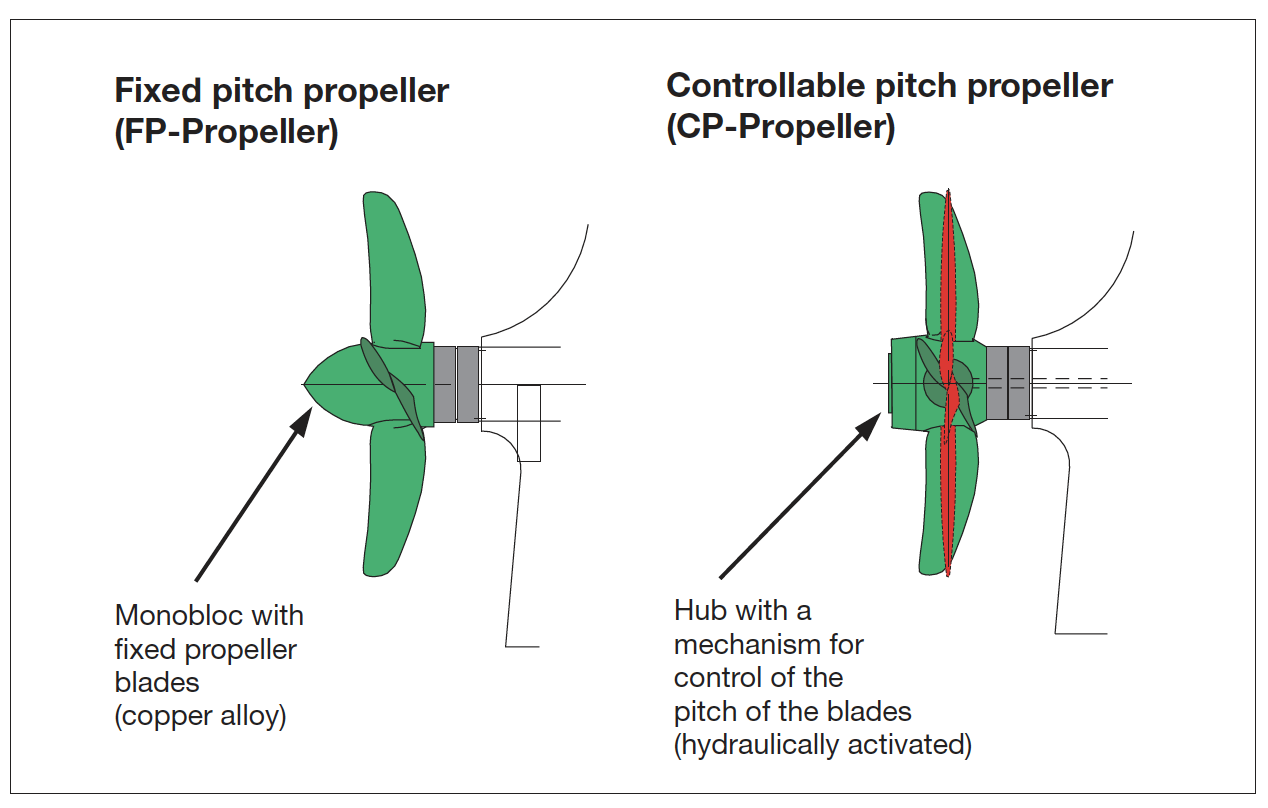
\includegraphics[width=\textwidth]{CPPropeller.png}
\caption{Controllable Pitch Propellers (CP Propellers) allow the pitch of the blades to be varied. Image credit: \parencite{mollard2011}}
\label{fig:CPPropeller.png}
\end{figure}

\subsubsection{Pitch and the Advance Ratio}
Pitch is also an extremely important concept to understand because it relates closely to the way that a propeller's 'open-water efficiency' $\eta_O$ is expressed in charts, as well as the advance ratio $J$ that usually comprises the x-axis in such charts.

\begin{figure}
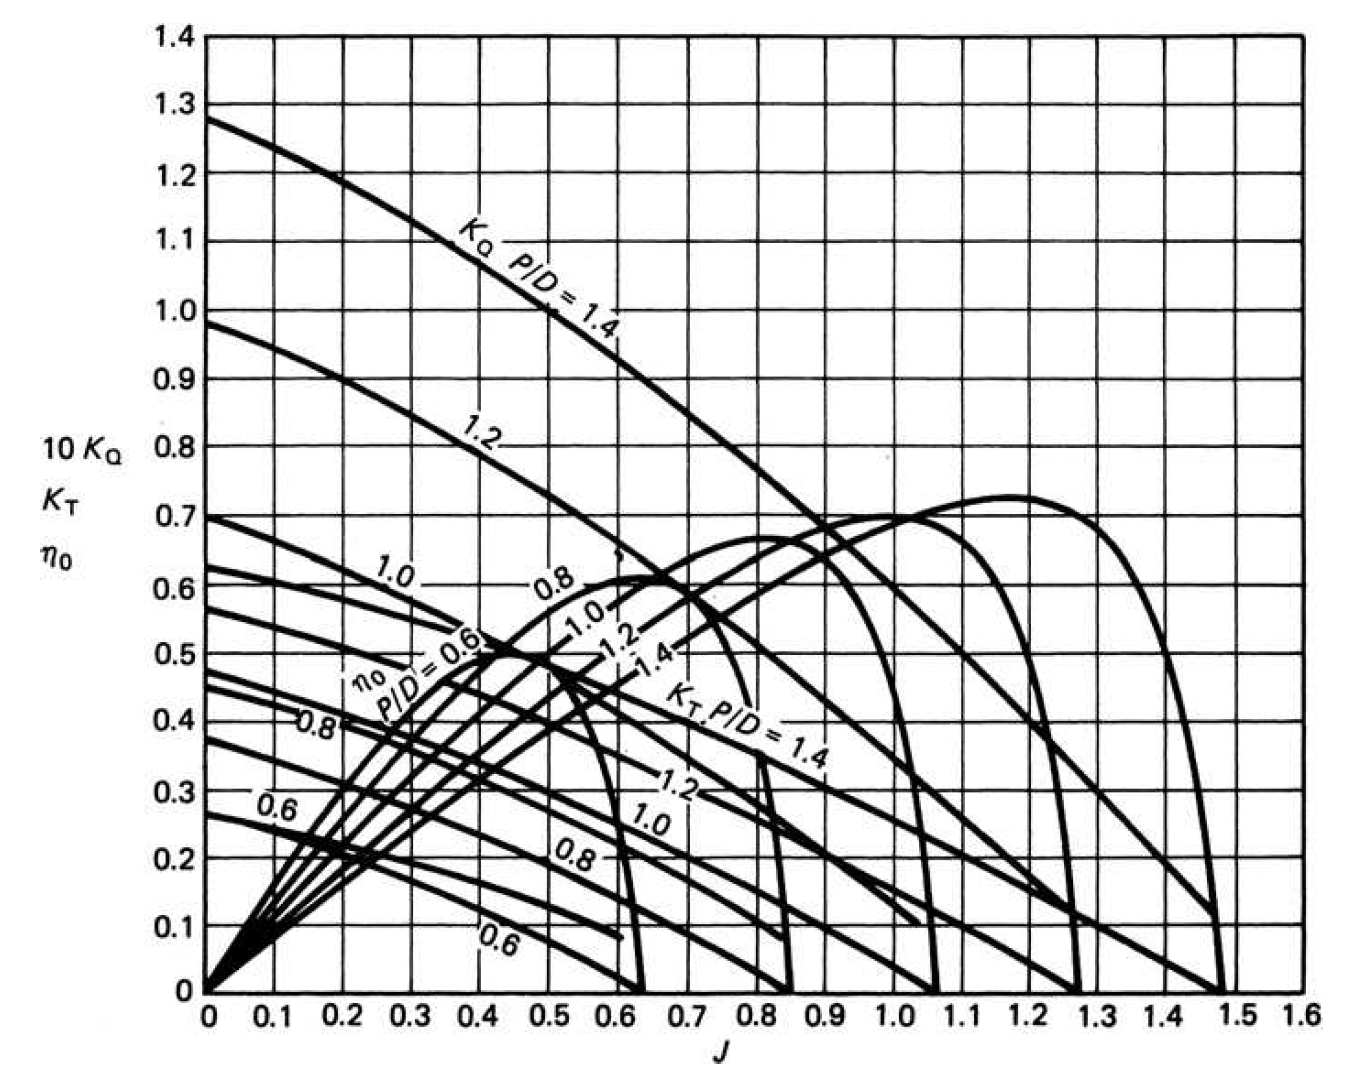
\includegraphics[width=\textwidth]{OpenWater.png}
\caption{A typical chart showing open water efficiency of a propeller, in this case a Wageningen B5-75. Image: MARIN}
\label{fig:OpenWater.png}
\end{figure}

This chart also shows two other closely related dimensionless coefficients, the torque and thrust coefficients ($K_Q$ and $K_T$) which we shall not dwell on here.  However, it is important to note that a number of different lines are expressed on this sort of chart, which represent different versions of the same propeller, with only the pitch (expressed in its dimensionless form as $P/D$) being different in each case. The x-axis, $J$, also warrants a clear definition:

\begin{equation}
\label{eq:2}
J = \frac{V_a}{nD}
\end{equation}

Where $V_a$ is the speed of advance of the propeller, or the speed at which water arrives at the front-side of the propeller, and $n$ represents the rate of the propeller's rotation (revolutions per second) and $D$ is the propeller's diameter.  For fullness of understanding it is also worthwhile to note here that $V_a$ does not correspond directly to the vessel's speed of travel, though they are related. To some extent, a vessel moving through water will always draw water in its wake along with it, which means that in the wake (where the propeller tends to operate to some extent or other) the water incident on the propeller will arrive at a lower speed than that implied by the ship speed \parencite[15]{MAN2017}.  Another key distinction for the consideration of jets later on, is that the speed of advance does not necessarily incporate the movement of water due to the movement induced by the propeller (or duct) itself, which is a distinct effect to that of the wake field. In \cite[213]{lewis1988} $V_A$ is used specifically to denote the undisturbed stream velocity, since the role of certain ducts can be to accelerate or decelerate the stream prior to the water arriving at the blades of the propeller.

One may also note from the previous figure that for each line representing a given pitch, the efficiency falls precipitously towards zero around the point where $J$ reaches $P/D$. This is because this extreme of the curve represents a circumstance where the propeller is rotating, but not actually moving any water, since it is moving through the water at about that speed which corresponds to the exact helical path defined by the pitch being traced. This represents circumstances where a propeller encounters effectively zero load.  This might be the case when a eases it's power, and the momentum of the ship temporarily keeps the ship moving without the propeller exerting much or any net thrust, or where alternative propoulsion sources (sails, or other propellers) are keeping a speed higher than what the propeller actually has push backwards on water to maintain.

A closely related concept here is the slip ratio, which is a measure of the difference between the pitch (the distance the blade section would travel if it traced a perfect helix for one rotation) and the actual distance that the blade did advance through the water.  This is neatly defined and shown in a diagram in \ref{fig:SlipRatio.png}.

\begin{figure}
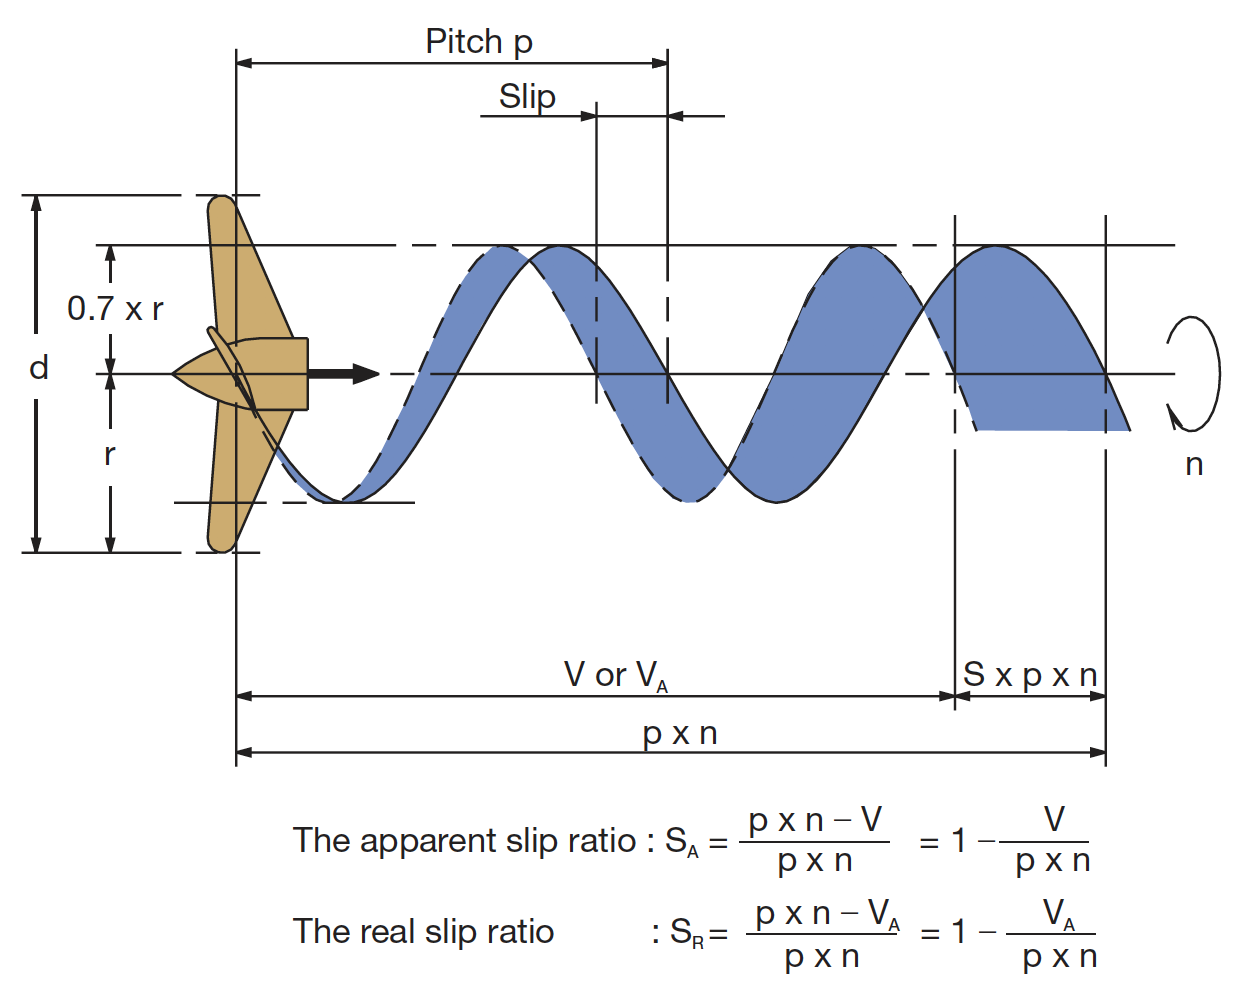
\includegraphics[width=\textwidth]{SlipRatio.png}
\caption{The slip ratio of a propeller. Image credit: \cite{MAN2017}}
\label{fig:SlipRatio.png}
\end{figure}

It can be seen from the diagram of the open-water efficiencies that there is some desirable non-zero slip ratio for a propeller.  The other end of the spectrum, where efficiencies also fall off toward zero, represent circumstances where the propeller is simply spinning in the same place in the water. In this case the slip ratio is one.  This represents a circumstance known as 'bollard pull' where a vessel is simply exerting force against an immovable object or infinite load.  Whilst the very low efficiencies here could represent a case of a propeller that is simply too small for the task it is trying to achieve, it is actually a significant and important circumstance to consider for propellers on working vessels such as tugs or trawlers, which exert large forces at very low water-speeds.  Measurement of the thrust generated in bollard pull, and the power required to achieve this thrust, is still an important metric for such vessels, but the definition of 'useful work' for normal propulsion requieres the thust to be excerted over some distance travelled.

\subsection{Ducted Propellers}
A ducted propeller is a propeller in any kind of tubular shroud, casing or nozzle.  Ducted propellers fall into broadly two categories, one of which is referred to frequently and interchangeably as a pump-jet.  The two types are called the accelerating type (also known as a Kort Nozzle, after a company that made them popular in the 20th Century) and the decelerating type.  The names describe the different effects that each type of nozzle have on the flow speed of the water at the point where it meets the propeller (which is also called an impeller, particularly when associated with decelerating ducts, or pumpjets).

A detailed description of the essential differences between the two can be easily demonstrated by diagram, which show a simple comparison an acelerating and decelerating duct, which have the shape of the aerofoil section which comprises the duct inverted. (Aside: It should be noted that some designs attempt to strike a balance between efficiency and cavitation performance of accelerating and decelerating ducts for certain purposes, and in such cases the duct shape might not be so clearly contrasted \parencite{abdel2010}.  But for the purposes of explanation, as well as optimisation for military purposes, the distinction between the two will generally be quite clear.)

\begin{figure}
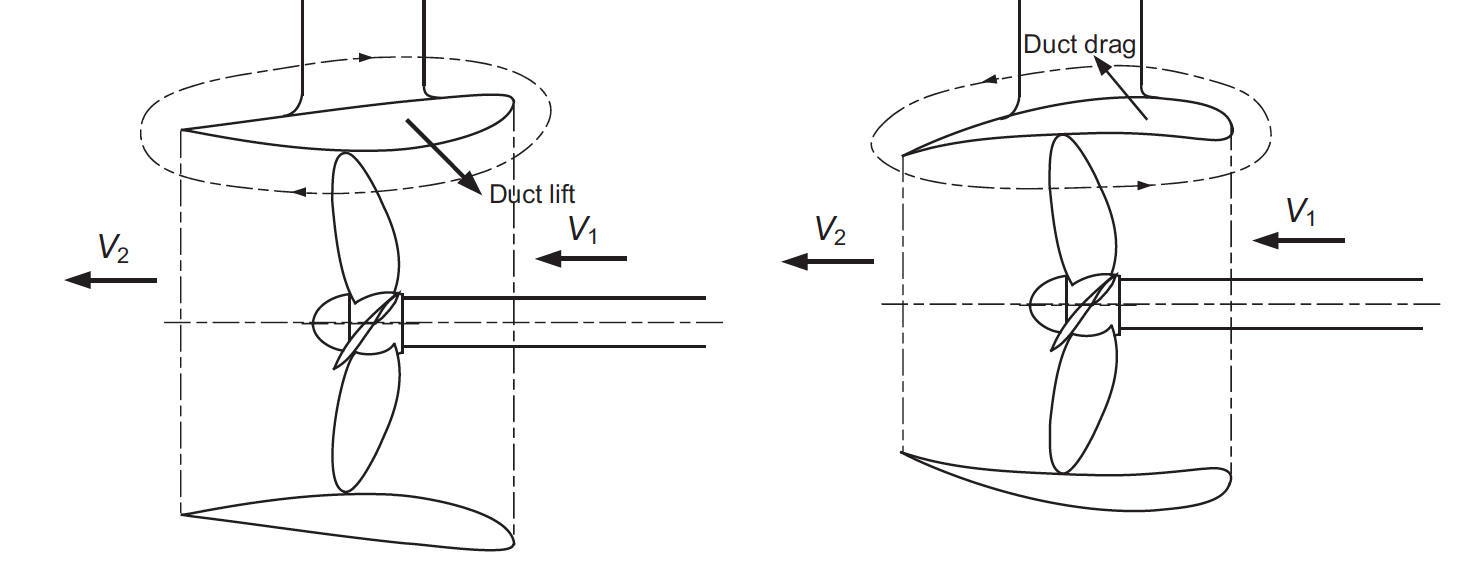
\includegraphics[width=\textwidth]{AccelDecel.png}
\caption{he two types of ducted propeller, accelerating (left) and decelerating (right) as shown in \parencite[249]{mollard2011}}
\label{fig:AccelDecel.png}
\end{figure}

A consideration of what happens to the flow as it moves through each type of duct helps to demonstrate how the acceleration and deceleration effects are achieved. In the case of an accelerating nozzle, the area through which the flow must pass contracts prior to the water arriving at the impeller.  In the decellerating case, the available area contracts after the water has passed the impeller. In some cases, a degree of diffusion is actually incorporated ahead of the impeller, whereby the area actually of the flow actually expands ahead of the impeller, which slows down the flow and increases its pressure according to Benoulli's principal \parencite{wislicenus1973}.

\begin{figure}
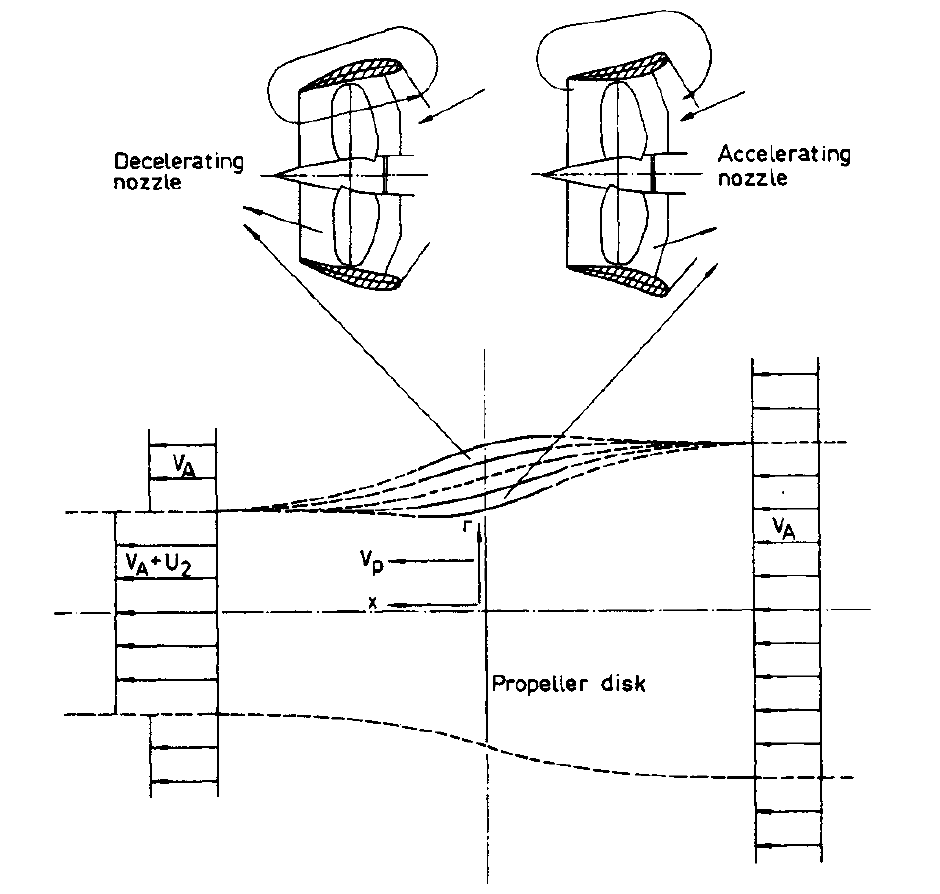
\includegraphics[width=\textwidth]{DuctStreamlines.png}
\caption{The streamlines of flow through different duct types \parencite[214]{lewis1988}}
\label{fig:DuctStreamlines.png}
\end{figure}

\subsubsection{The Accelerating Duct}
Accelerating ducts are most commonly used by vessels which have to operate at high loadings at very low speed, such as tugs, barges, or trawlers.  In those circumstances, relatively small vessels need to exert considerable forces against substantial loads, at very low water-speeds.  Also, in these circumstances, the practical size of a propeller might be constrained, since operating an optimally sized propeller might increase the complexity of machiner required to deliver the power to so low a hub in the water, and it might also be difficult to arrange for the thrust to be directed substantially against the centre of drag of the vessel.

The effect of the nozzle in these circumstances actually increase the optimal efficiency of the propeller, when operating at very low water-speeds, since the pressure reduction on the inside of the nozzle induced by the movement of the water through the nozzle, actually produces a net thrust forward, since the interior face at the opening of the nozzle is necessarily angled forward. This has the effect of distributing the suction force across a larger area, which now includes the interior of the nozzle.  An equivalent way of describing the same effect is that the nozzle causes the water to be accelerated more gradually, over a longer distance, by inducing it to move more quickly as it passes through to the entrance.  As a broad generalisation, more gradual or gentle actions tend to involve lower overall losses to turbulence, and hence the efficiency of the propeller can be increased.

A further means by which the efficiency of a propeller can be increased is through the reduction of the turbulence created by the blade-tips passing through the open (static) water at high speed.  Since the two sides of the blades have low and high pressure on them respectively, at the tips where the two faces meet, there there is a tendancy for water to 'spill' from the high pressure side the the low pressure side, creating a vortex which leads to unwanted turbulence.  It is also around this vortex that blade tip cavitation tends to occur. By limiting the movement of water around the outside of the blade tip by having a tightly fitted shroud, losses due to this particulary type of tubulence, and the onset of this type of cavitation can be diminished.

However, it is important to note that the existence of an accelerating duct by no means eliminates all cavitation.  In fact, given that the static pressure at the impeller is necessarily reduced by an accleratint duct, the propensity for cavitation other surface of the propeller is generally increased, and cavitation can and does still occur in ducted propellers near the blade tips \parencite{moulijn2015}.

\begin{figure}
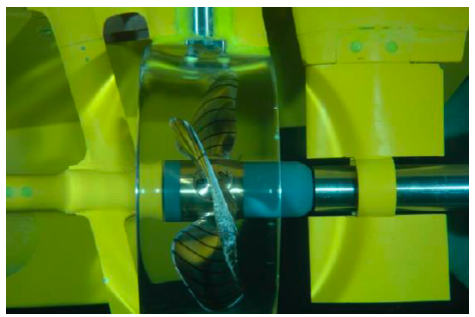
\includegraphics[width=\textwidth]{CavitatingDuct.png}
\caption{An example of the cavitation occurring at the blade tips of a ducted propeller. Image credit \cite{moulijn2015}}
\label{fig:CavitatingDuct.png}
\end{figure}

A detailed explanation of the means by which the ideal efficiency of propeller can be improved can be found in \cite[213-222]{lewis1988}, as well as other texts on marine propulsion, such as \cite{carlton2007}. A substantial work exploring the efficiencies of a range of accelerating and decelerating ducts can also be found in \cite{oosterveld1970}.  A common feature of these extensive studies also show that for ducted propellers, including accelerating ducted propellers, the advantage in terms of efficiency is overall restricted to low waterspeeds.  At higher waterspeeds, the drag induced by the water-movement over the exterior of the duct begins to increase substantially, and the net thrust on the duct becomes negative.  When the exterior of the duct experience relatively little water velocity, but the interior experiences a great deal more, the greatest advantages of an accelerating duct are realised.  Furthermore, in general these models do not incorporate the effect of flow separation, which is acknowledged as a possibility on both the exterior and interior of ducts, which can dramatically reduce efficiency performance (\cite[20]{oosterveld1970}, \cite[214]{lewis1988}).

\begin{figure}
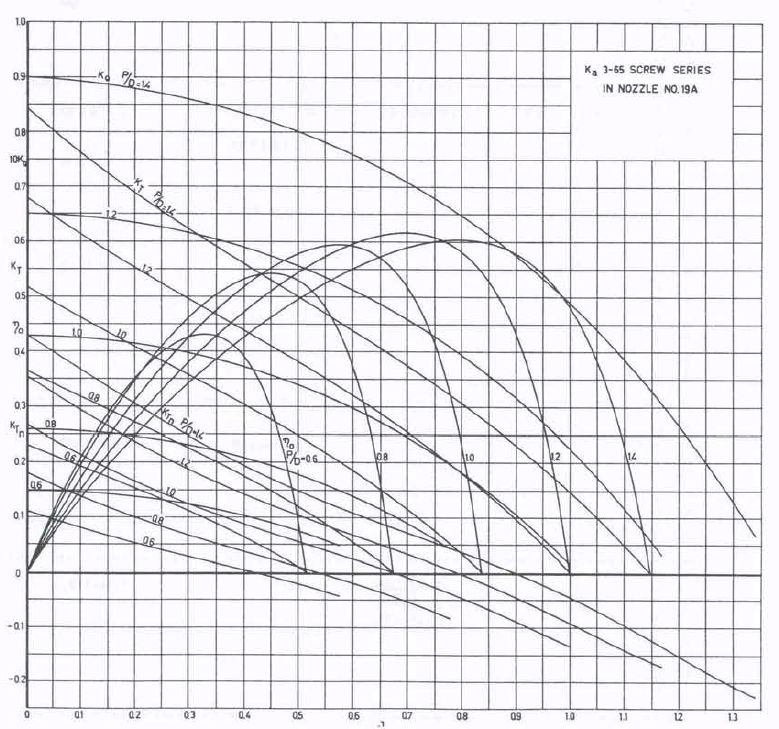
\includegraphics[width=\textwidth]{DuctedEfficiency.png}
\caption{Accelerating ducts produce a net positive thrust at low advance ratios, but a net negative thrust at higher advance ratios as the drag on the nozzle exterior increases. Image credit:Open-water test results of Ka 3-65 screw series with nozzle no. 19A \parencite{oosterveld1970}}
\label{fig:DuctedEfficiency.png}
\end{figure}

\subsubsection{The Decelerating Duct or Pumpjet}
Decelerating ducts necessarily produce a negative thrust, since the process of raising the pressure of the water about the impeller (equivalent to slowing it down) necessitate reducing its kinetic energy and consequently momentum.  In a wide range of literature introducing the fundamentals of ducted propellers and water-jets, or discussing their more modern development there is universal acknowledgement that the choice of a decelerating duct is generally made for the avoidance of cavitation for specialised (generally military) purposes, rather than for the achievement of increased efficiency (\cite{carlton2007}, \cite{oosterveld1970}, \cite{mollard2011}, \cite{haimov2010}, \cite{lewis1988}).

In order to achieve a reduction in cavitation, however, care must be taken in the design of a decelerating duct.  Since the negative thrust produced by the duct must necessitate additional work being done by the impeller, there can be circumstances where the additional loading of the impeller out-weighs the impacts of elevating the pressure around it. \cite[24-25]{oosterveld1970} provides a more thorough derivation of the circumstances in which this can be reliably achieved, which generally include larger blade area ratios or with more rows of rotors for higher loading, or circumstances where the loading of the propeller is quite low.  This creates an inevitable and necessary tension between optimisation of a duct for propulsive efficiency and reduction of cavitation, which will be returned to in subsequent section.

It is perhaps most relevant at this point to further clarify the distinction between the different names for related or similar systems.  In \cite[17]{carlton2007} pump jet is described as an "interesting development of the classical ducted propeller". Oosterveld, in his thesis on ducted propellers also states with regard to the decelerating duct "This ducted propeller system is the so called pumpjet" \parencite[8]{oosterveld1970}.  Other authors give separate treatement to ducted propellers and pump jets, though the systems they describe are essentially similar in terms of composition, advantages, and physics \parencite[288]{lewis1988}.

\begin{figure}
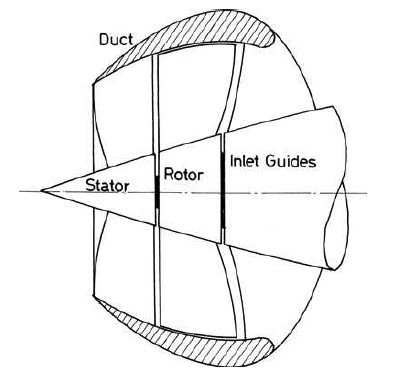
\includegraphics[width=\textwidth]{PumpjetOutline.png}
\caption{In \cite{carlton2007} the pump jet is described as a development of a classical ducted propeller, with the noticeable addition of a stator}
\label{fig:PumpjetOutline.png}
\end{figure}

In other definitive literature on the design of pumpjets \parencite{henderson1964} the difference between a pumpjet and a propeller is a described as being that "the stream of flow through the pumpjet is made to depart from the "natural" or free-stream sufrace that bounds the flow though a standard propeller."  According to the diagrams and the subsequent description it is clear that the definition embraces quite exactly the distinction between an accelerating duct, and a decelerating duct, namely that the flow is slowed at the point it encounters the impeller, where as in a free situation the free stream would contract at this point.

The addition of some new part such as stator blades (to straighten out the flow) and other possible features which make the propeller system more like pump or turbomachinery components might be associated with systems more commonly referred to as pumpjets than ducted propellers. The key concepts behind the operation of these systems, however, remains essentially similar in their nature and design intent.

\subsubsection{Waterjets}
The use of the word waterjet, as opposed to pumpjet, signifies that the jet expelled from the shroud or pump is situated above the water, which is desirable in very fast-moving surface vessels which attempt to minimise their contact with the waters surface, including high-speed planing hull vessels, including pleasure craft.  The physics of the two systems, however, are closely related, with the very noticeable exception of the absence of flow considerations for water on the exterior of the duct considerations for waterjets.  However, the physics relating to the impeller and stator blades or (turbomachinery) designed to add energy to the flow are generally extremely closely linked, though a larger variety of diffeent pump types can be chosen for waterjets which might differ more significantly from the natural evolution of a propeller to an axial-flow pump. Many of the essential equations which govern the efficiencies and cavitation performance of pumpjets and waterjets are of the same or extremely similar form, as can be seen in detailed discussions given to both, by similar authors (\cite{wislicenus1973}, \cite{henderson1964}).  There are, however, plenty of instances in recent literature where this distinction regarding the ejection of the jet above and below the waterline is not maintained, and waterjets and pumpjets seem to be used interchangeably \parencite{abdel2010}.

\begin{figure}
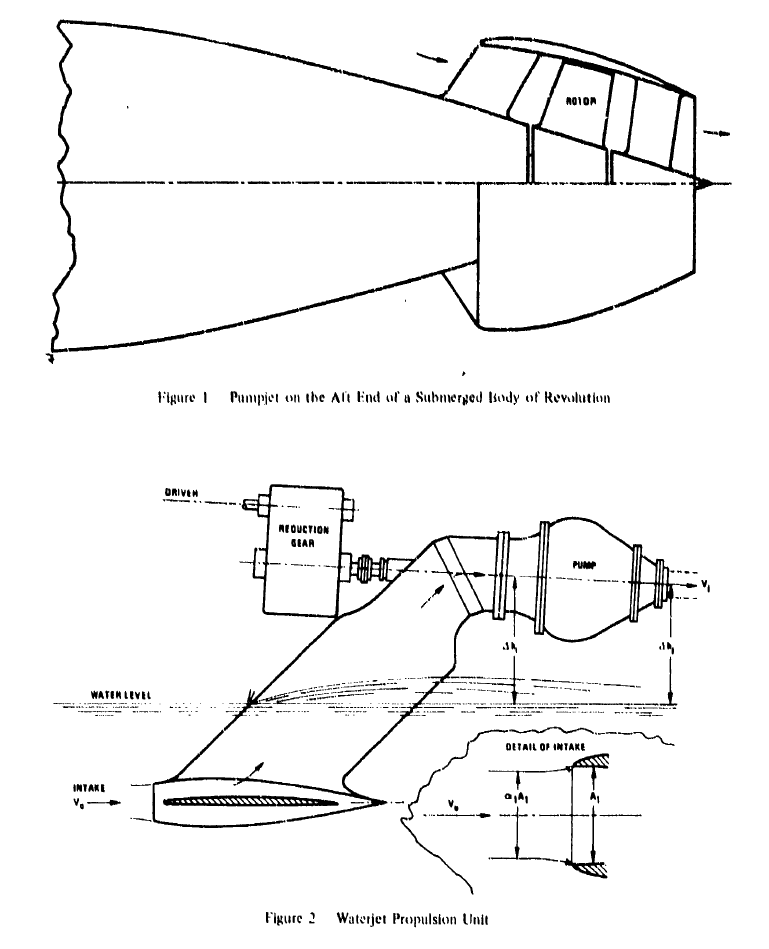
\includegraphics[width=\textwidth]{PumpjetWaterjet.png}
\caption{A comparison of a pumpjet and waterjet as given in \cite{wislicenus1973}}
\label{fig:PumpjetWaterjet.png}
\end{figure}

\section{Constraints on the efficiency of pumpjets at low speed}

\subsection{Recent Commentary}
There has been already some attention given to the probable efficiencies of pump jets at low speed. Recently Andrew Davies published a piece in the The Strategist (ASPI) arguing that the pump jet may actually save fuel at transit speeds (around 8kt) and overall improve the endurance of the submarine, despite likely having lower efficiency at low speeds such as patrol speed \parencite{davies2017}.  This argument relies pump-jet efficiency still overtaking that of propellers at what is considered a relatively low speed for many applications.  As Andrew acknowledges, further quantification of the likely efficiency is required, as the particular chart which he cites is not quantified.  This section aims to identify as far as is reasonably possible from public literature how the efficiency of a likely pump-jet for a submarine might perform in quantitative terms, relative to a propeller.

There has also been questions put in parliamentary hearings regarding the pump jet \parencite{patrick2017} and responses from public officials to such questions indicate that some of the literature provided to support such lines of questions was dated, and that the state of the art may have advanced considerably since this time.  Whilst the argument that the state of the art is much advanced is obviously true, it is the case with marine propulsion, as with most sciences, that new developments tend to confirm, rather than annul, many of the workings that have been previously undertaken.  To the extent that modern literature still supports the overall constraints and bounds provided by some of the foundational earlier works, a great deal of useful information can still be obtained from earlier works.  In particular, the foundational theories, often derived from well-established principals of conservation of momentum, energy, as applied by the likes of Bernoulli and Euler, are as well respected and deeply depended upon today as they were centuries earlier when they were first arrived at.

\subsection{Modern literature and results}
In addition, more modern works, including those which involve experimental validation of theoretical results also tend to show that restrictions on the efficiency of waterjets are enduring, and give us a clear starting-point for consideration of their probable orders of magnitude, and likely transition points indicating at what speeds pumpjets might become advantageously more efficient.

A 1995 Japanese experimental study on the performance of a waterjet demonstrated a close experimental fit to a theoretical relationship which sees the propulsive efficiency of the waterjet fall to zero with craft velocity, with significant declines in efficiency commencing just under 10m/s, or somewhere around 18kt \parencite{fujisawa1995}.

\begin{figure}
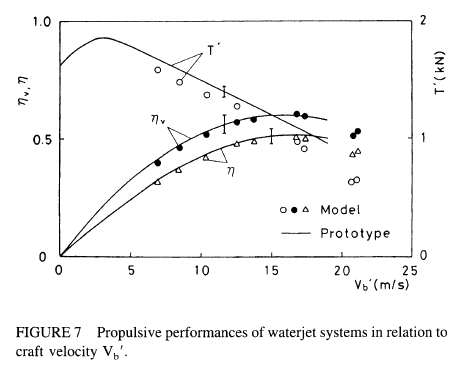
\includegraphics[width=\textwidth]{EfficiencyJapan.png}
\caption{A graph from a Japanese study of waterjet efficiency shows efficiency rapidly declining below craft velocities of 10m/s, in accordance with theory. \parencite{fujisawa1995}}
\label{fig:EfficiencyJapan.png}
\end{figure}

In 2015 an Australian team including staff from the Australian Maritime College and Incat published results of an experimental study comparing the use of waterjets and propellers for medium-speed ferries operating in the 20-30kt speed range \parencite{kamal2015}.  This study explicitly set out to establish the cross-over point for where propellers become more efficient than jets, since Incat was interested in pioneering highly efficient medium-speed vessels, after having considerable success in very high speed catamarans.  It is again acknowledged as given that at lower speeds propellers are more efficient than waterjets.  The study found that propellers were considerably more efficient over the entire speed range tested, often by a factor of two in terms of transport efficiency.

\begin{figure}
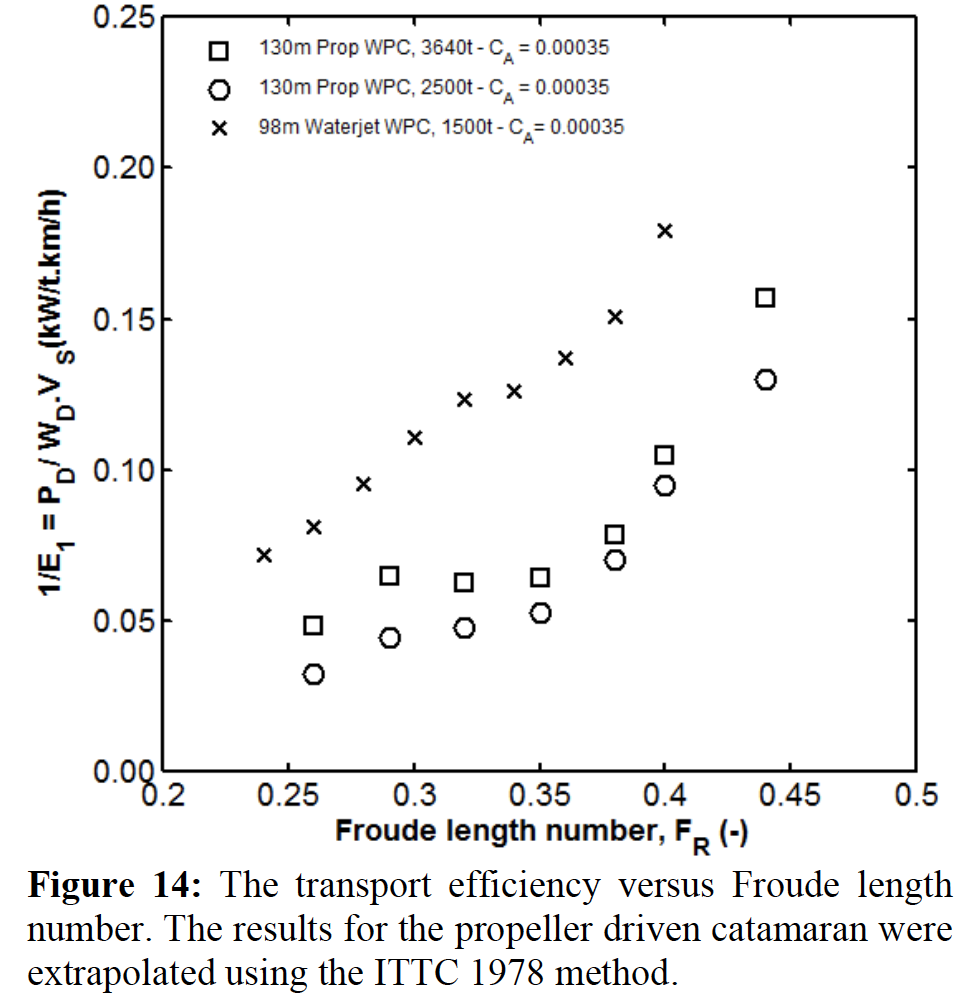
\includegraphics[width=\textwidth]{EfficiencyTransport.png}
\caption{An Australian experimental study aimed at determining the crossover point for the efficiency of jets and propellers in the 20-30kt range revealed much higher power was required across the entire speed range \parencite{kamal2015}}
\label{fig:EfficiencyTransport.png}
\end{figure}

Both of these previous studies confirm the general and widespread assumption that jets are known to be more efficient at high speeds, and propellers at lower speeds.  They also suggest that differences in efficiency could be very large, of a factor of two or more, including at speeds well over a submarine's transit speed.  However, care must be taken making precise quantitative comparisons, since such experiements involved jets which expelled into air (waterjets) as opposed to remaining under water (pumpjets). Pumpjets would experience drag on the exterior of the shroud/duct, which waterjets would not, however waterjets are likely to have longer intake ducts, which might involve larger duct losses than pumpjets.  Given that these factors might affect efficiency, and the overall design of the nozzle considerably, more direct comparison with fully submerged jets should be sought to make more direct comparisons.

At IMARESTS 10th International Naval Engineering Conference, a paper was presented by BMT Defence and Rolls Royce \parencite{giles2010}, outlining a proposal for 'fully submerged waterjets' to be used on future surface ships in order to achieve better acoustic performance, particulalry for an anti-submarine warfare role. The jets comprise a mixed-flow pump coupled to an electric motor, and have been both extensively modelled and also tesed in demonstrator vessels.  These may be a closer representation of the performance characteristics achievable by submerged pumpjets, since shape of the intake and shroud more closely resembles the shape of a pumpjet that might be found on a submarine.  Importantly, this work focuses specifically on the performance of the jets as a function of ship-speed, including identifying possible crossover points.

\begin{figure}
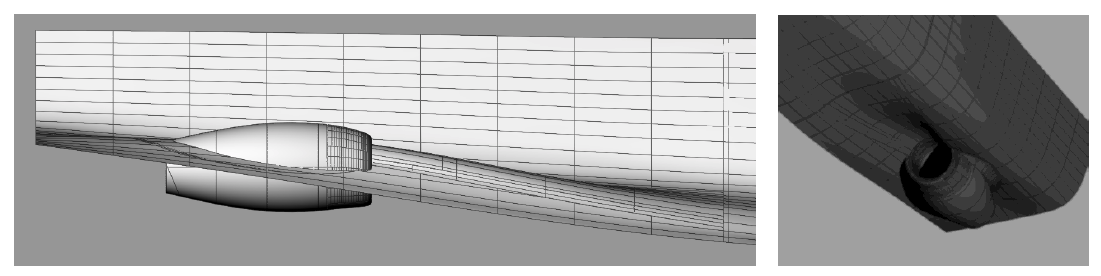
\includegraphics[width=\textwidth]{BMTShape.png}
\caption{The 'fully submerged waterjet' proposed by BMT and Rolls Royce for military surface craft may more closely represent the duct shape used on submarines than waterjets that release above the surface. \parencite{giles2010}}
\label{fig:BMTShape.png}
\end{figure}

The paper makes no effort to justify the selection of choice of jets on the efficiency of the propulsion system, instead focussing on improved acoustic performance, and potential machinery space-saving advantages.  The vessel under consideration would require 250 tonnes more fuel with jets find than with propellers, the jets would require more power to reach equal waterspeed to a conventionally propelled craft right up to 30 kt.  In the case of this analysis, modifications to the hullform in order to accommodate the jet (which are likely to be more substantial for a surface ship than a submarine) also have an impcat on the resistance offerd by the hull.  This also has an interaction with the different shape of the propulsors, which alters the required level of delivered (effective) power to achieve a given speed, in addition to the considerations of how efficiently the propulsor generates that effective power. The paper states: "This is an encouraging result for a first iteration as the AWJ-21™ arrangement has not been fully optimised and, hence, there is further prospect of reducing the shaft power for this form. If the power could be reduced by 5\% (e.g. by fur ther improving the waterjet/hull fairing), then the AWJ-21™ vessel would be better at all speeds above 25 knots."  This statement, however, is made in reference to the hullform needed to accommodate the jet, rather than the jet itself. \parencite{giles2010}

The paper also provides specific curves for the efficiency of the propulsor as a function of vessel speed, which demonstrated that the waterjet efficiency was lower than that of conventional propellers throughout the speed range, but declined particularly precipitously below speeds of 10kt.  At 5kt, the propeller was more than twice as efficient as the waterjet.

\begin{figure}
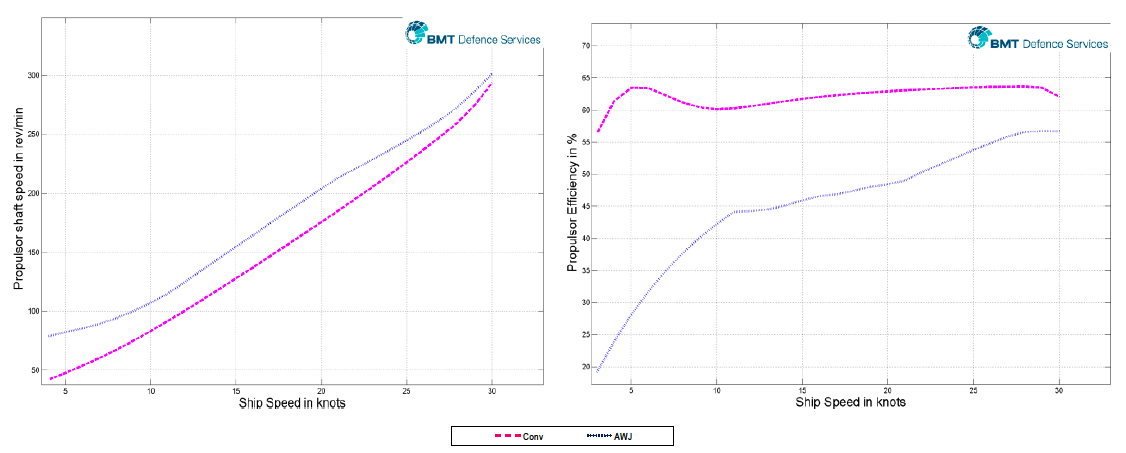
\includegraphics[width=\textwidth]{BMTEfficiency.png}
\caption{Studies on submerged waterjets for military surface craft currently show that the efficiency of jets decline sharply below 10kt \parencite{giles2010}}
\label{fig:BMTEfficiency.png}
\end{figure}

It appears from recent examples in the literature that there is no evidence of jets approaching the same efficiency as propellers at speeds as low as 10kt.  Indeed, there seems to be considerable evidence that jets of most kinds suffer substantial efficiency penalties relative to propellers in this regime, and that this is understood and accepted as an inevitable design trade-off to be made.  In the case of a submarine, which might spend nearly 100\% of its time travelling at 10kt or less, this disadvantage (as opposed to less than 35\%, as assumed for a surface ship) would become extremely substantial, which will be quantified in later sections.

Moreover, recent literature seems to confirm that efficiency of pumpjets fall off precipitously towards zero the closer that the vessel speed comes to zero.  This strongly suggests the existence of some fundamental constraint in the physics of the operation of jets, which recent advances in technology seems not to have overcome.  To more firmly establish the extent to which adaptation or plausible improvments in technology could or could not change this trend, it is worthwhile considering the theoretical limits that are presented by the physics.  This should further limit the range of error that might be made in estimating realistic bounds of performance for an unknown system.

\subsection{Theoretical Limitations}
In this section I will appraise some of the available literature, including some of the most canonical works in the design of pumpjets which is now declassified from US Navy funded research (and still extremely frequently cited by contemporary researchers).  Before doing so, I'll attempt to summarise in simple language the mose essential conclusions in simple language.

My broad conclusion is that the optimisation of a system for minimising cavitation, and hence improving acoustic performance, is a separate and independent design requirement to that of optimising a system for propulsive efficiency.  These two design requirements can be found either to be in tension, or alignment, in different regimes.  At high speeds, where cavitation tends to have severe impacts on propulsive efficiency of open propellers, and high mass-flow (which leads to good efficiency) can be achieved through compact ducts and pumps, pumpjets offer very good performance on both metrics.  Hence, in this regime the two design requirements tend to align relatively well in favour of pump-jets.  However, in very low-speed, low-load environments, where cavitation effects are negligible, and larger areas need to be engaged achieve good mass-flow and efficiency, the two design requirements align relatively well in favour of an open propeller.  In a variety of intermediate regimes, the two requirements find themselves in tension.

For this particular consideration, two questions are of paricular importance.  The first is where the clear transitions in the regimes will tend to lie, with respect to the probable requirements of a conventional submarine.  The second is what drives the tension between those design requirements in the intermediate regimes, and whether it is a fundamental or inescapble tension in the laws of physics, or simply a technical hurdle which imminent improvements in the state of the art are likely to overcome by engineering improvements or innovation.

The answer to the first question, as discussed in earlier sections, seems to be that the operating speeds of a submarine tend to lie far below the probable levels where pumpjets are even remotely comparable to waterjets for efficiency.  In later sections I will address further the acoustic comparisons in the speed ranges at 10kt and below.

The answer to the second question seems to be that there the tension between acoustic and propulsive performance at intermediate speeds and loadings is driven by foundational physical requirements.  That is not to say that optimal means of balancing those requirements will not still be found, and improved, as the art advances.  However, it does mean that significantly adapting using known variables that can be changed to favour one design requirement are unlikely to yeild large improvements without some trade-off being made to the other.

The reason for this trade-off occurring can be quite simply attributed to the nature of the shroud, or duct, which surrounds the the rotors of the propulsor, and the effect it has on the flow. If the duct acts to increase the pressure at the rotor, (which reduces cavitation) it necessarily must slow the flow at/around the rotor, which necessitates produceing a negative thrust on the duct.  The system as a whole produces a positive thrust, becuase the impeller or rotor pushes a larger positive thrust, but the duct necessarily produces a negative thrust.  At the speeds get lower, and the thrust required gets much much lower, this negative thrust becomes proportionally more significant, as described later.

Put another way, the work required to slow the water down, then speed it up again, becomes a gradually greater penalty the the slower the water is coming in, and the less you actually want to speed it up.  If the water is slowed enough by the duct to effectively stop, then the impeller must do the work of speeding it up (sucking it into the duct) before the duct slows it down, before the impeller raises its pressure, and the pressure accelerates it out of the nozzle afterwards. Compared to simply accelerating the water in one simple push, as a propeller blade does in an unconstrained flow, the efficiency penalty is very large.

\subsection{The impact of duct loss on an ideal propeller}

Derivations of the 'ideal' efficiencies are frequently made for propellers, and jets using basic conservation laws (momentum theory) which consider simply acceleration of some column of water as actuated by a disc representing the impeller or propeller.  A fuller description of these equations can be found in  most standard texts \parencite[131]{lewis1988}. These methods are computationally simple, and allow simple upper-bounds to be be set for efficiencies achievable for given designs under certain conditions, without considering the portential impact of other more complex effects such as skin friction over the blades, potential flow separation, or cavitation.  As such, they can be easily relied upon to constrain the overall plausible range of values that can be achieved from universally applicable inputs, such as the velocity of water going into a duct, and the velocity of water exiting a nozzle.

Such methods are used in \cite[8-14]{wislicenus1973} to construct an 'ideal' jet efficiency that applies to waterjets and jetpumps. Whilst I won't repeat the full expansion here, but a fundamentally important early conclusion of the derivation is the distinction between 'useful work' and the total energy expended. since the rate of change in momentum is known to be necessarily equal to the force generated, and increasing momentum change (hence thrust) can be achieved either accelerating more mass, or accelerating mass to higher speeds.   Given that energy embodied in a flow is proportional to it's velocity squared, but its momentum only to its velocity, a necessary and inevitable consequence is that some energy is always wasted in accelerating a fluid to a higher velocity than its surrounds.

This is expressed in the equation which represents 'ideal jet efficiency', which is directly equivalent to 'ideal propeller efficiency' using momentum theory of propeller action:

\begin{equation}
\label{eq:3}
\eta_j = \frac{1}{1+\frac{\Delta V}{2V_0}}
\end{equation}

The inevitable consequence of this relationshiop is that efficency approaches unity when $\Delta V$ (the change in water of the water between entering and exiting the system) relative to $V_0$ approaches zero.  Intuitive embodiments of this relationship are (equivalently) that efficiency is maximum when the least force is exerted on any given bit of water, which might be when negligibly small work is being done (extreme low speed) or when such a large mass of water is acted on that it barely needs to be pushed at all.  This relationship would lead to the conclusion that infinitely large propellers or jets are always desirable from an efficiency perspective.  This of course isn't practical to build, and also doesn't hold when the effects of the drag on the propeller blades, or duct, are taken into account.  Infinitely large systems would increase the total weight, as well as having significant surface draw when moving through the water, all of which are neglected in this 'ideal' consideration.

In \cite[8-14]{wislicenus1973}, Wislicenus expands the relationship in the case of the jet to incorporate terms to represent some of the inevitable adjustments that would occur in the case of pump jets and waterjets, particulalry the duct head loss ($K$) (fraction of energy required to push the water through the duct), as well as the additional drag on the outside of the propulsor ($\Delta T$).  This leads to an adjusted efficiency relationship, which still neglects any losses due to pump efficiency, or change in height of the jet (which is added for consideration for waterjets, but not relevant here).


\begin{equation}
\label{eq:4}
\eta_j = \frac{1}{1 + \frac{\Delta V}{2V_0} + K\frac{V_0}{2 \Delta V}}(1 - \frac{\Delta T}{T})
\end{equation}


The conclusion of the analysis, and the plotting of these results for certain possible values of $K$ and $\Delta T$ is: "Its outstanding characteristic is that this efficiency approaches zero rather than unity for $\Delta V / V_0 = 0$, even for small duct losses".

\begin{figure}
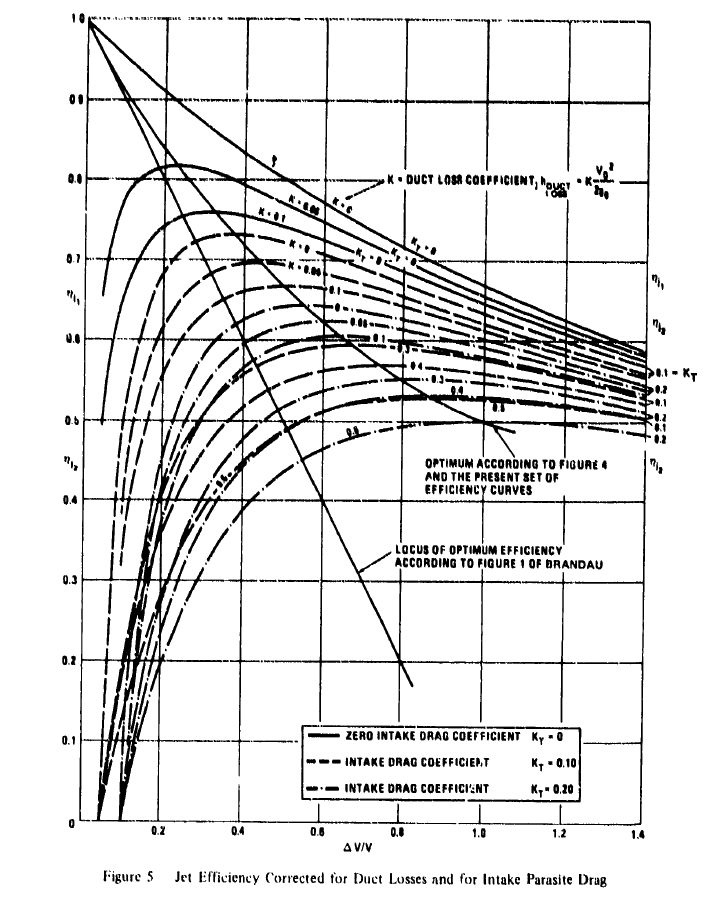
\includegraphics[width=\textwidth]{PumpjetEfficiency.png}
\caption{Ideal jet efficiencies sharply appoach zero at low values of $\Delta V / V_0$, where as ideal propeller efficiencies without a duct $K = 0$ approach unity. Credit: \cite{wislicenus1973}}
\label{fig:PumpjetEfficiency.png}
\end{figure}

Wislicenus also acknowledges \cite{wislicenus1973} another author, Brandau, who makes a different assumption about the relationship between the duct loss and water velocity \parencite{brandau1967} in his derivation (along with another thorough discussion of potential and ideal efficiencies), who produces a different peak efficiency point, but retains a similar overall shape featuring efficiency falling very rapidly to zero at low values of $\Delta V / V_0$, and contrasting this with the ideal propeller, which approaches unity in this low regime.

It's important to note at this point that whilst charts such as these are generally used with dimensionless ratios on the axes (such as $\Delta V / V_0$) to allow the most general solutions to be used to solve for any given particular vessel size, speed, or loading requirement which might be required, these  confusing to many readers unfamiliar with hydrodynamics.  For the avoidance of any confusion, for a particular fixed vessel size and drag, and fixed propulsion system design smaller values of $\Delta V / V_0$ will correspond to to the propulsion system exerting less thrust, and also moving at a lower speed under self-propulsion, since the thust required (proportional to $\Delta V$ when operating at steady state) will decline faster than the vessel speed or water speed at intake, since the drag on the vessel scales with the square of the vessel speed.

\begin{figure}
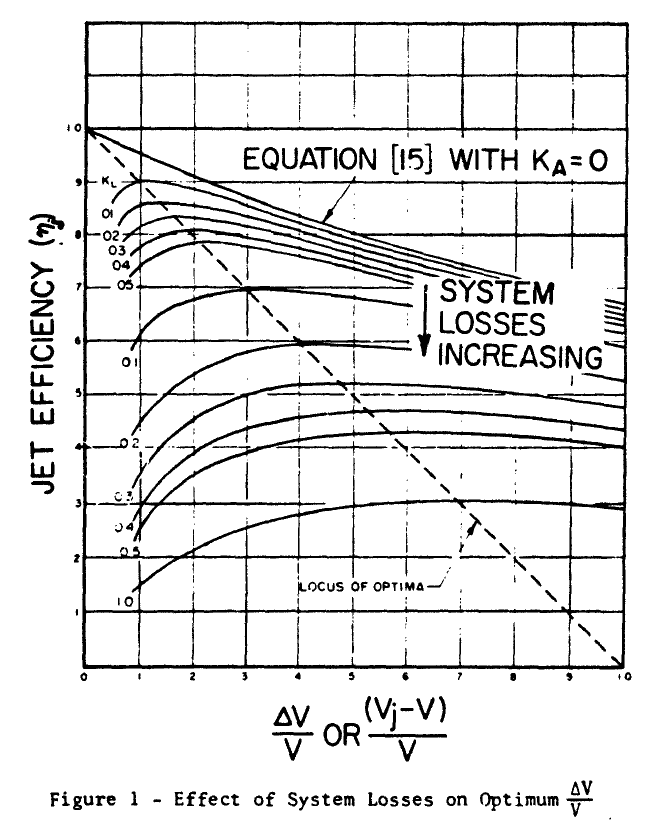
\includegraphics[width=\textwidth]{EfficiencyBrandau.png}
\caption{Alternative derivations of ideal jet efficiency also show sharply declining efficiency for low values of $\Delta V / V_0$ Credit: \cite{brandau1967}}
\label{fig:EfficiencyBrandau.png}
\end{figure}

The structure of these overall curves is found to be overall quite similar for both pumpjets and waterjets, though the probably values for the losses incurred in the intake duct, or on the exterior of the shroud, are obviously different \parencite[13-14]{wislicenus1973}.  Similar efficiency shapes can be found for discussions focussing explicitly on underwater pumpjets \parencite[13]{henderson1964}. It should be noted that the theoretical efficiency derived by these general equations is consistent both in derivation and results with those produced by other authors \parencite[227]{lewis1988}.

Care should be taken, however, to note that different graphs for efficiency can be produced which have different variables on the x axis.  For example, \cite[247]{mollard2011} a graph of ideal efficiency of a pump jet is shown using the speed of advance divided by the jet speed, or $V_1/V_2$.  Given that the x axis used in the previous charts used $\Delta V / V_0$, which would be related to $V_2-V_1$ in this case, this has the effect of reversing the effective direction of the chart. In this case, for a fixed jet and vessel design, high-speed operations will be towards the left of the chart, and the precipitous decline in efficiency will occur as speed declines to zero, along with thrust, toward the right of the chart, as opposed to the left in earlier cases.

\begin{figure}
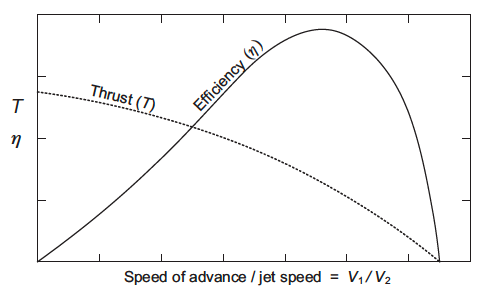
\includegraphics[width=\textwidth]{EfficiencyMollard.png}
\caption{Other modern reference texts might demonstrate jet or propeller efficiencies with different x-axes, effectively reversing the way the graph should be understood for a single system operating at different speeds. Credit:  \cite{mollard2011}}
\label{fig:EfficiencyMollard.png}
\end{figure}

\begin{figure}
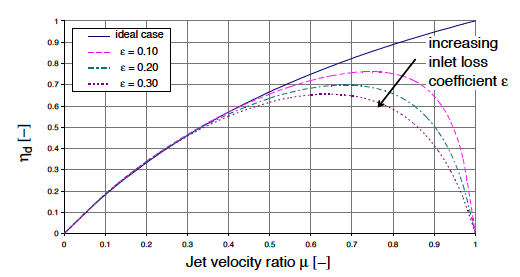
\includegraphics[width=\textwidth]{EfficiencyBulten.png}
\caption{Another graph representing efficiency as a function of the ratio of jet velocity to incoming velocity, which shows efficiency declining at low thrust (to the right).  The impact of increasing duct losses can be clearly seen, as opposed to the 'ideal' propeller without a duct. Credit: \cite{bulten2006numerical}}
\label{fig:EfficiencyBulten.png}
\end{figure}

Similarly, it is very important to note that the very frequently used x-axis unit $J = V_a/nD$ when showing efficiency curves for both propellers and ducted propellers (such as used in earlier figures) are of a similar orientation to the chart shown in the figure above.  The left side of the chart will correspond to the highest number of rotations for a given amount of progress through the water.  For vessel of fixed load, and a propeller of fixed geomtry, this will correspond to a propeller facing the higest drag force due to the vessel moving at the highest speed.

Readers may observe that the efficiency for all propellers also decline to zero at the other end of the spectrum, most sharply at a point where $J$ equals or exceeds the pitch ratio of the propeller.  As discussed earlier, these correspond to cases where the propeller is slicing along its helical path without exerting any force to move water backwards, or when the slip ratio is zero.  In this circumstance, the rotation of the propeller would not push any net water backwards, and simply act as a paddle-wheel needlessly spinning water.  Such circumstances are unlikely to occur to a significant degree unless a vessel was decelerating, or experienced some other force to assist its propulsion.  It is possible that at extremely low speeds a propeller could somewhat descend to the right of optimal advance ratio, when very dramatically reduced load was encounterd because of the extreme low speed, as might be suggested by the slight reduction in propulsive efficiency of the propeller below 5kt in the BMT study.  The conclusion if design at no higher speeds was required that using a smaller propeller area, which accelerated slightly thicker slices of water with each blade, would re-optimise efficiency.  These losses of efficiency, however, could never supercede those of a decelerating ducted propeller or jet, which has the shroud which necessarily imposes an \textbf{additional} drag to the watercolumn in excess of any other resistance faced by the rotor.  This effect can be seen clearly even or an accelerating duct, as shown in \ref{fig:PropDuct.png}.

\begin{figure}
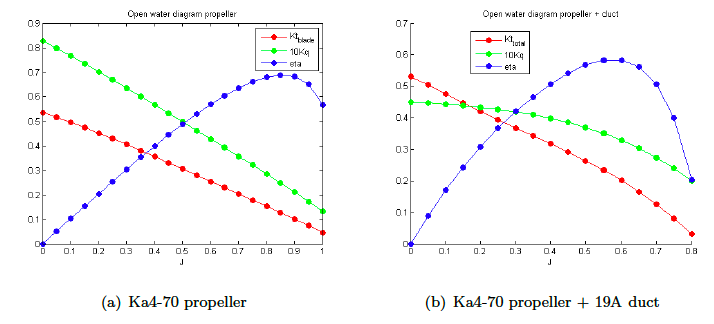
\includegraphics[width=\textwidth]{PropDuct.png}
\caption{Even the addition of an accelerating ducts substantially reduces efficiency of propellers at very low loadings, or for constant loads, low speeds.  Maximum attainable efficiency is also reduced. Their benefit lies in the bulging of the curve at low advance ratios (higher loads).  Credit: \cite[6]{willemsen2013}}
\label{fig:PropDuct.png}
\end{figure}

It should be clear from the above analysis that the efficiency of a pumpjet falling towards zero with a vessels waterspeed is an enduring and foundational result of basic physics.  The addition of negative thrust on a decelerating duct, no matter how small, necessitates that efficiency must decline at some point with with blade loading, in contrast with an ideal propeller which rises to unity.  This explains the overall shape given by the the mysterious unquantified chart cited by Andrew Davies \parencite{davies2017} and Access Economics \parencite{stanford2017} shown \ref{fig:PumpUp.png}, and also matches the shapes plotted by more recent studies as shown above, and also the shape presented in other modern publications studying the use of pumpjets \parencite{giles2010} and waterjets \parencite{fujisawa1995}.

\begin{figure}
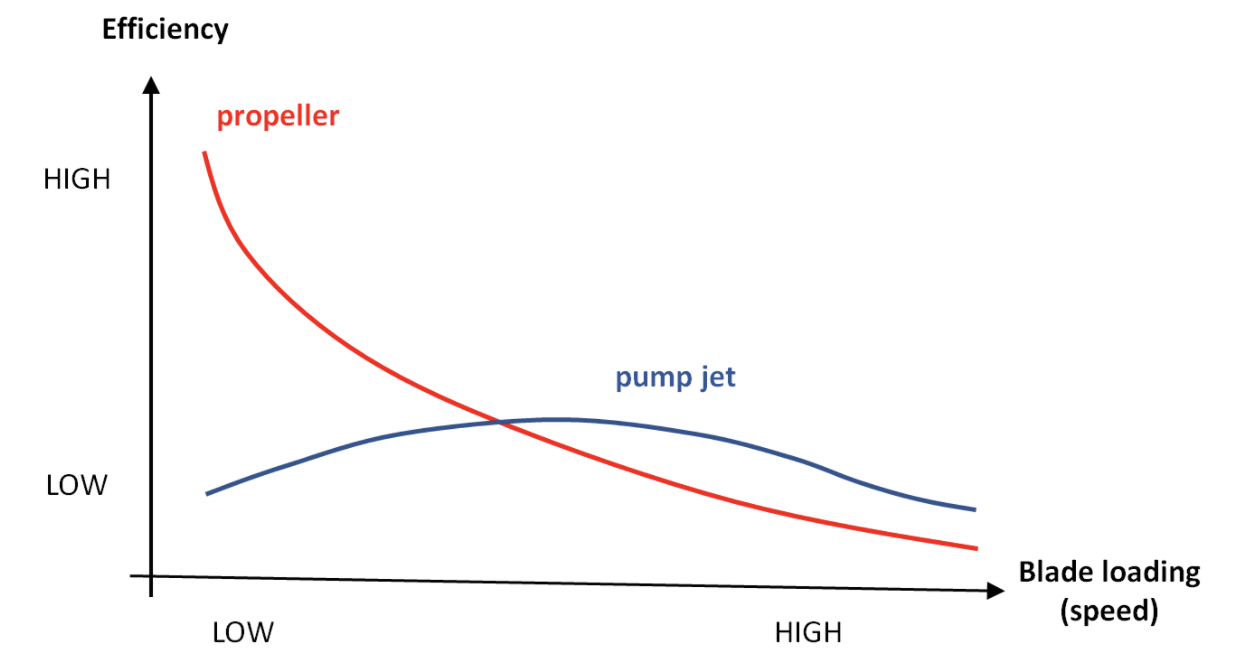
\includegraphics[width=\textwidth]{PumpUp.png}
\caption{The mysterious efficiency comparison chart which has been doing the rounds in the Australian debate probably quite reasonably reflects theoretical physical limits of 'ideal' pumpjets and propellers. Credit: \cite{stanford2017}}
\label{fig:PumpUp.png}
\end{figure}

In terms of establishing plausible peaks and cross-over points, the study undertaken in \cite{giles2010} probably provides a sufficient indication as to the current state of the art in the relevant technologies.  Whilst this effort focussed on a surface vessel rather than a   The study was undertaken with the backing of military customers with support and testing facilities (the US Navy), and involved two major companies who are world leaders in maritime engineering (BMT) and waterjet manufacture (Rolls Royce). Even if further technical advances through design refinement were possible, as the authors alude to, the cross-over point in terms of efficiency might be brought down to 25kt.  The prospect that the crossover point lies anywhere near the transit speed of a convetional submarine (8-10kt) appears utterly implausible. In discussions with leading world experts involved in the development of advanced ducted propellers (including those involved in citations) I was told that a pumpjet could not be more efficient than a propeller below 18kt.

With the optimum efficiency of a jet probably being no greater than 60\% or 70\% at its peak efficiency according to many theoretical and experimental studies \parencite{lu2016cfd}, which would quite probably lie considerably higher in terms of waterspeed, these facts, along with the inevitable decline of efficiency towards zero as waterspeed also declines, a suitably constrained set of plausible efficiency curves may be investigated numerically, as will be done later in later sections.

\subsection{An assessment of scope for improving the efficiency of a pumpjet at low speeds}
Before continuing to assess the impact of the likely efficiency curves of pumpjets relative to propellers, it is worthwhile considering what the known literature about the theory of pumps, jets, and turbomachinery might tell us about the potential for a radical advance which make might substantially improve the shape of the curve at very low speeds.  Whilst the field of propulsor design is no doubt complex, and I will not attempt to be exhaustive in detailing all of the potential design considerations which might make an improvement.  However, the pursuit of reasonably comprehensive confidence is aided by the the scale of the gap which probably needs to be closed to make pumpjets comparably efficient to propellers at the relevant speeds.  Minor adjustments and the improvement of small or marginal effects, of which there might be many, will clearly not help in shifting the efficiency peak of a jet from over 25kt to under 10kt.  In other words, this gap will not be closed or noticeably reduced by 'tuning'.  Quite substantial redesign of core characteristics (like mass flow) would be required, which would necessitate a cycle of redesign and tuning virtually all other aspect of the entire jet, as illustrated by numerous guides to the design of such systems (\cite{bruce1974}, \cite{furuya1988}, \cite{mccormick1963design}, \cite{henderson1964}).  As such, I will only consider those parameters which could plausibly be altered quite substantially, where the consideration of larger changes make the likely limits or trade-offs quite clear.

\subsubsection{Increase mass-flow by widening area of intake}
Perhaps the most obvious means by which one might attain substantial increases in efficiency is to increase substantially the mass flow rate.  This is derived from a fundamental relationship, as expressed earlier in the representation of ideal propeller and jet efficiency (prior to the consideration of any drag or other losses) which was given in the earlier equation.  Since excessive velocity differences result in more energy expended than momentum changed, as given by momentum theory and basic mechanics, doing work on a large body of water, rather than working harder on more of it, is generally desirable from an efficiency perspective.  Considering what the appropriate mass-flow should be at design speeds is generally the first thing that is specified to occur in all design processes for pumpjets, and good example of which is in \cite[6-7]{henderson1964}.

As Henderson et al. note, the key constraint of this variable is that increasing the diameter of the pumpjet necessarily leads to an increase in the surface (including the external suface) of the shroud.  The increased drag that this induces must be deducted from the thrust that the pumpjet produces, or effectively increasing $\Delta T$ as given in earlier equations.  In this respect, there is "no free lunch" to be had in expanding the size of the intake.  As Henderson et al. conclude, for this reason the diameter of a pumpjet tends to be about 15\% or 20\% smaller than that of a corresponding propeller, whereas the diameter to have equivalent mass-flow, highlighting the tension set up in pumpjet design with their earlier observation that "if the cavitation resistance of the blades is to be improved with no reduction in thrust and the same rate of flow through the propulsor, the pump jet rotor must be larger than that of the propeller." \parencite[1]{henderson1964}

It should also noted that in order to substantially increase the opening area of the propeller, the difference between the velocity of movement at the blades nearer to the root (close to the hub) and the extremities of the blades increases substantially.  In order for equivalent work to be done on all of the water distributed radially across area of the impeller, quite a different blade shape might be required, in order to provide a higher deflection of the water close to the root. In these areas, there is increase probability of flow separation occurring, where the velocity of movement of the water across the surface is insufficient to overcome the pressure gradient required to move over the blades.  (In a pump, the pressure necessarily increases as work is done on it.)  Or, since there isn't enough pressure exerted on the whole of the water column to overcome the resistance imposed by the duct, not all of the water moves forward, and some starts to move backwards.  This leads to flow separation, or stall occurring close to the blade roots, which dramatically diminishes the efficiency of the system. A further discussion of this effect can be found in \cite[15,27]{henderson1964},  \cite[807,8012]{bruce1974},  \cite[185]{wislicenus1973}, \cite[60]{mcbride1979} and many other related texts.  This is a general problem that affects a range of axial-flow turbomachinery, particulalry operating in off-design conditions, and will present a general concern for the design of a new pumpjet \cite[185]{wislicenus1986}, \cite{li2013}.

\begin{figure}
\includegraphics[width=\textwidth]{stall.png}
\caption{Flow separation, or stall, can occur when the flow over the blades of a pump slows too much, as shown in \cite{li2013}}
\label{fig:stall.png}
\end{figure}

\begin{figure}
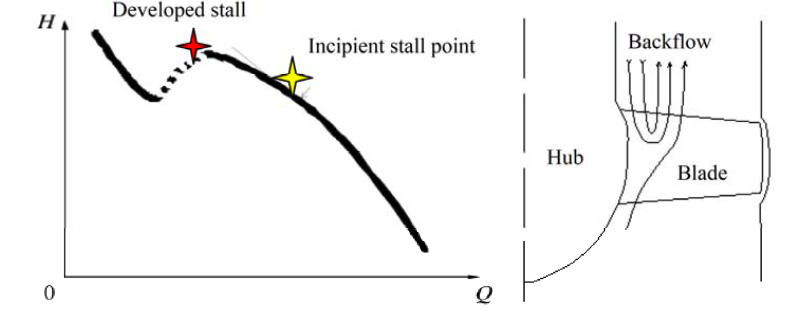
\includegraphics[width=\textwidth]{backflow.png}
\caption{Stall results in water flowing backwards near the hub of the blades at low flow rates, as shown in \cite{li2014rotating}}
\label{fig:backflow.png}
\end{figure}

It is possible to limit the variation of deflection between the blade tips and roots by simply expanding the size of the hub.  However, this necessarily reduces the effective frontal area that is available to receive the mass-flow, which necessitates further expansion of the outer diameter, and a very substantial increase in the weight of the system.  In addition, expansion of the hub will necessarily increase the total surface area relative to the mass flow, including by increasing the amount of tapering required after the stators in order to prevent risk of cavitation occuring around the hub.

Increasing the frontal area of the intake also is necessarily linked to the advance ratio of jet.  Since low advance ratios correspond to higher shaft speed for a given forward velocity, increasing the thrust produced for a given rotation (by widening the jet area) necessarily results in higher advance ratios, since more work is done on the water for a given rotation. However, this also necessarily results in poorer cavitation performance of the jet, since higher blade velocities relative to the water flow result in necessarily increased propensity for cavitation.  A detailed discussion of this can be found in \cite{gearhart1966selection}, but similar tensions can be readily found in most other pieces of literature, including \cite{henderson1964}, \cite{wislicenus1973}.

Given the fundamental nature of the flow-rate and intake area to the design of pump-jets, and the great lenght of time for which they have been understood and discussed as a crucial design input for a waterjet, it is altogether implausible that some large increase in intake area can be achieved without incurring necessary and unavoidable tradeoffs.

\subsubsection{Reduce degree of diffusion (i.e. switch to accelerating duct) to reduce negative thrust from duct}
A further means of reducing the negative thrust produced by a duct may involve significantly reducing the degree of diffusion, or compression that occurs in advance of the rotor, since the process of diffusion necessarily slows the water and produces negative thrust.  However, this amounts to transitioning towards an accelerating duct, or Kort Nozzle. Whilst nozzles of this type have been known to improve the cavitation characteristics of a propeller by enclosing the tips (which often tend to cavitate first), their ultimate function is to actually decrease the pressure at the blades of the propeller.  Consequently, they necessarily increase the propensity of other types of cavitation to occur across the blade-face, including bubble, cloud and sheet cavitation. As such, these types of propellers are not considered for the military purposes which require an absolute minimum of noise to be created.  Transitioning to an accelerating duct signify a shift away from a pump-jet, and necessarily be in direct tension with the need to minimise cavitation for acoustic considerations.

In addition, whilst it is often demonstrated that for a given propeller under certain load conditions (high loading), the addition of an accelerating duct can considerably improve efficiency, all of these situations have generally been in the context of vessels which are designed for a relatively high thrust, low waterspeed situation, when propeller size is necessarily somewhat constrained.  This is the case fishing vessels, or for tug boats, which need to impart significant thrust to a vessel dozens or hundreds of times their own size.  Mounting a propeller the equivalent size of the vessels they mean to push, however, would be excessively heavy, arranging a mount and power drive that would keep the entire propeller submerged, and not have the effect of flipping the boat backwards when pushing hard, would be effectively impossible, without proportionally increasing the size of the tug. Furthermore, in most circumstances these propellers are still designed to operate with some cavitation, even if the extent of it is reduced by the presence of the duct \parencite{haimov2010}.

In other words, the use of highly loaded propellers in such applications is actually particular to design constraints that are unlikely to be present for a submarine, which can position the propeller at the tail of its body, directly behind its centre of mass and drag, and consequenlty have freedom about the optimal size of the blades.  It is well known that a duct cannot improve the performance of a low-loaded propeller which would be the situation for a slow-moving vessel with unconstrained propeller size.  Authoritative references in the literature include \cite{oosterveld1970}, who calculates the minimum thrust coefficient $C_T$ (a measure of loading) for an accelerating duct to improve a propellers performance to be between 1 and 2, as shown in @AcceleratingIdeal.

\begin{figure}
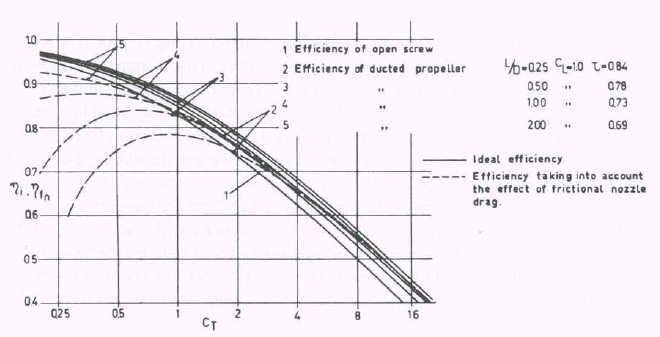
\includegraphics[width=\textwidth]{AcceleratingIdeal.png}
\caption{Calculations of 'ideal' efficiencies of accelerating ducts (neglecting drag) in \cite{oosterveld1970} show that a duct can only improve the efficiency of a propeller if it is loaded above a certain degree, and that longer ducts produce better improvements in 'ideal' efficiencies}
\label{fig:AcceleratingIdeal.png}
\end{figure}

A parallel design change in the switch away from the degree of deceleration in the duct would be the reduction of the nozzle contraction after the rotor.  For waterjets and pumpjets of all sorts, based on fundamental disc actuator theory, the degree of this contraction of the flow area has also been long identified as a means to increase pressure at the rotor, and hence decrease cavitation, but at the direct expense of efficiency \parencite[14]{van1996waterjet}.

Numerous efforts to find suitably compromised duct shapes exist, but even advanced modern designs still exhibit declining efficiency at low speeds, as well as some cavitation during operations at design loads, which still tend to imply relatively high speeds, for example 27kt in \ref{fig:FineOptimised.png} .  Consideration of accelerating duct designs for a military submarine would be extremely unlikely, and be a profound departure from any existing pumpjet designs.

\begin{figure}
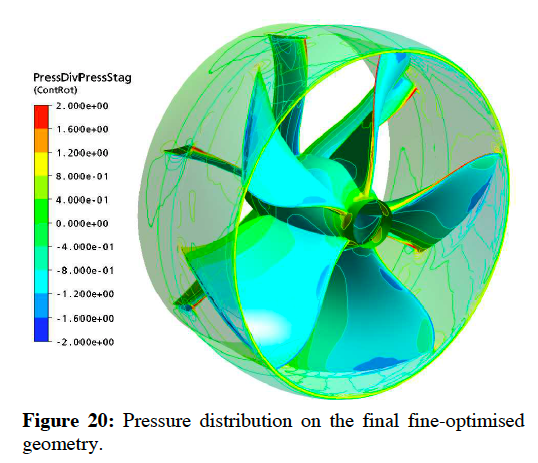
\includegraphics[width=\textwidth]{FineOptimised.png}
\caption{Extensive work has been done exploring compromise designs for decelerating ducted propellers (pumpjets), including with very modest deceleration in the intake, limited shroud taper, short duct lengths, or essentially incporate some of the advantages of accelerating ducts. Credit: \cite{abdel2010}}
\label{fig:FineOptimised.png}
\end{figure}

\begin{figure}
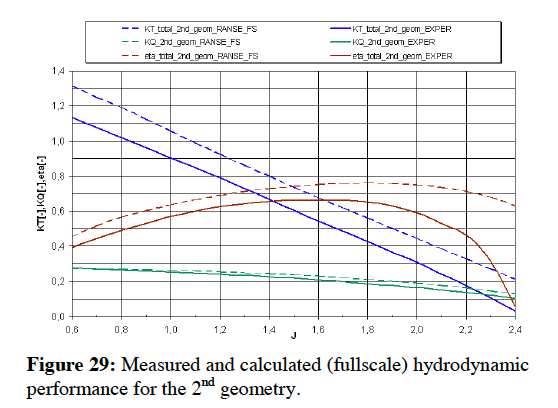
\includegraphics[width=\textwidth]{FineEfficiency.png}
\caption{In experimental testing such designs still exhibit sharply falling effiency at high advance ratios, or low speed. Credit:  \cite{abdel2010}}
\label{fig:FineEfficiency.png}
\end{figure}

\begin{figure}
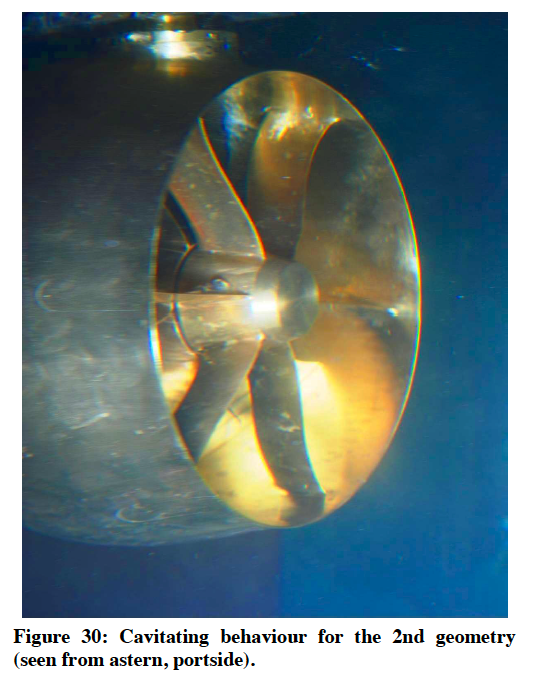
\includegraphics[width=\textwidth]{FineCavitation.png}
\caption{TAt optimally efficient conditions (corresponding to 27kt) such designs still exhibit some cavitation. Credit: \cite{abdel2010}}
\label{fig:FineCavitation.png}
\end{figure}

\subsubsection{Reduce shroud length to decrease drag on duct}
The reduction of the length of the shroud in order to reduce drag presents another possible means to lower the duct resistance, as shown and discussed in \cite[21-25]{oosterveld1970}. The fundamental difficulty with greatly shortening a duct, however, is that it requires that any changes in the shape and with of the water column be accomplished much shorter distance for the duct to achieve its desired effect, which means that generally it has to achieve less of it.  This means that extremely very low duct lenght achieve less of an efficiency improvement to the ideal efficiency of a propeller, in those circumstances where they can achieve an improvement  (accelerating ducts), as discussed above.

If more aggressive shape changes are attemped in a limited space, the deflections of flow and pressure gradients become much more extreme. This leads to a far greater propensity for flow separation to occur.  This can happen inside the duct ahead of the stator, particulalry when any degree of diffusion occurs in order to elevate static pressure at the blades, or any kind of direction change is required as in the case of waterjets. Unlike waterjets, pumpjets also have the potential for separation on the exterior surface, which is an additional concern in the design of duct \cite[13]{henderson1964}.  Given the role of the duct is to change the speed of the flow at the impeller relative to what would occur in its absence (in particular to decelerate it) separation might tend to occur on different surfaces in different operating conditions, depending on the relative pressure gradients and velocity ratios they experience at different speeds and loads.  This substantially complicates the challenge of designing a duct that performs well across a wide speed range. This is illustrated for the case of a waterjet in \cite[20]{bulten2006numerical}.  Equivalent complexities occur in pumpjets operating in low speed ranges (2-6kt, where flow separation occurs ahead of the impeller, inside the shroud.  In the case of an accelerating duct, this phenomenon is also observed at high advance ratios, or the equivalent of low speeds and low loads, as shown and discussed in some detail in \cite{willemsen2013}.

\begin{figure}
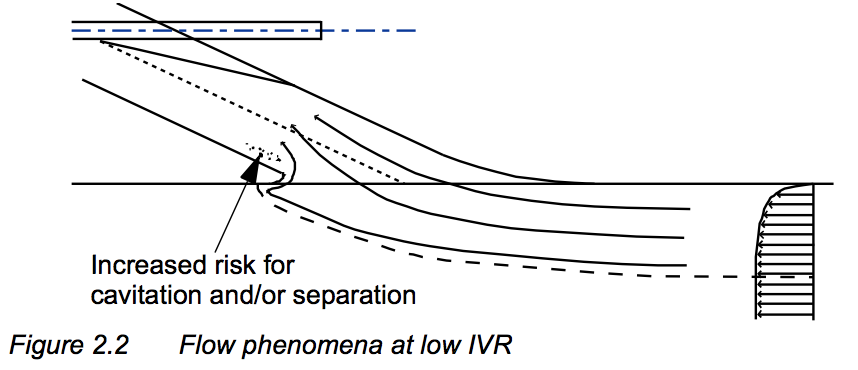
\includegraphics[width=0.5\textwidth]{LowIVR.png}
\caption{A an intake may experience risks of flow separation even at low speeds (Inlet Velocity Ratio) on some surfaces due to certain flow deflections being more severe. Source: \cite{bulten2006numerical}}
\label{fig:LowIVR.png}
\end{figure}

\begin{figure}
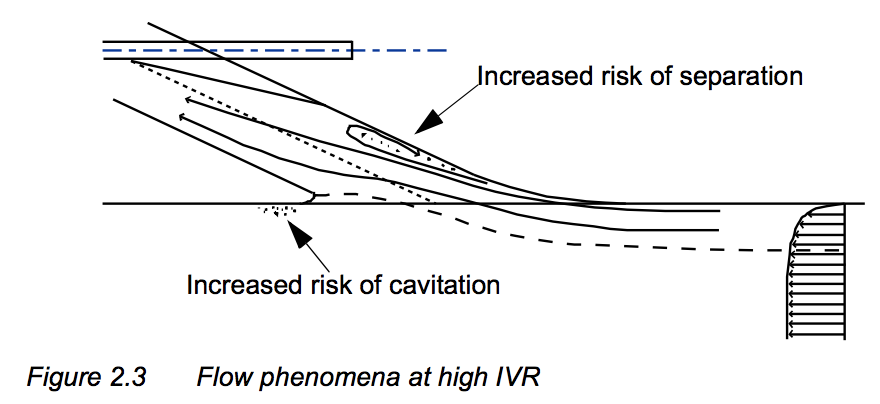
\includegraphics[width=\textwidth]{HighIVR.png}
\caption{A an intake may experience risk of flow separation on different surfaces at high speeds (Inlet Velocity Ratio) where other flow deflections are more severe. Source: \cite{bulten2006numerical}}
\label{fig:HighIVR.png}
\end{figure}

\begin{figure}
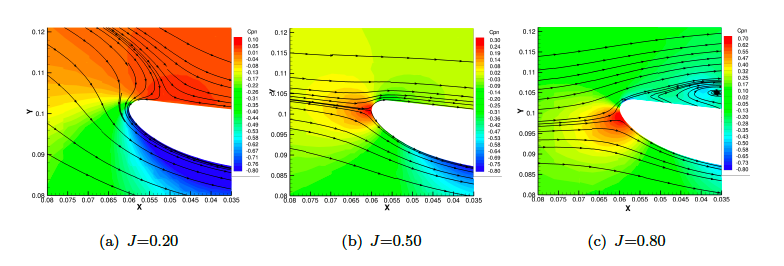
\includegraphics[width=\textwidth]{DuctSeparation.png}
\caption{Flow separation occurs at on the outside of an accelerating duct at high $J$ values, which corresponds to low loads, or speeds. For high $J$ values, the pressure reduction on the inside of the duct, creating positive duct thrust, can be seen. Source: \cite[73]{willemsen2013}}
\label{fig:DuctSeparation.png}
\end{figure}

\begin{figure}
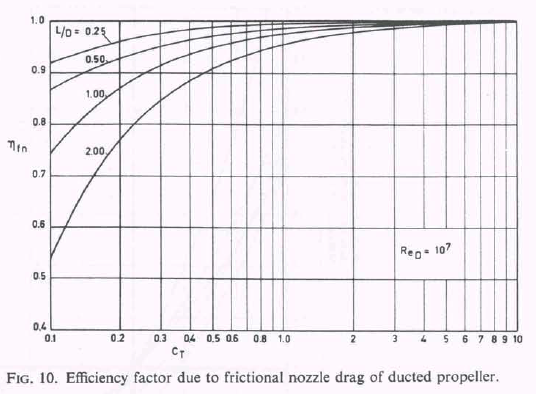
\includegraphics[width=\textwidth]{NozzleDrag.png}
\caption{Dramatically reducing the length of a duct relative to its diameter ($L/D$) as shown in \cite{oosterveld1970} can reduce its drag, which has the most significant impact at low thrusts or speeds.}
\label{fig:NozzleDrag.png}
\end{figure}

In addition, the substantial reduction in the length of the shroud, both ahead of and behind the rotor, will also have the substantial effect of diminishing any acoustic sheilding which the duct may achieve.

\subsubsection{Summary remarks on potential for redesign of pumpjet for low-speed conditions}
Overall, while the parameter-space for the alteration of marine-propulsors is large, the parameters which would allow for very dramatic rather than minor changes to propulsor efficiency at low speed are relatively few.  The major ones include increasing the width of the intake, decreasing the length of the duct, and decreasing the pressure inrease at the blades achieved by the duct.  In short, it involves evolving the pumpjet back towards a propeller.  None of these changes could be effected to a substantial degree without some inevitable trade-off in terms of the cavitation performance of the system at higher speeds.

\section{Model Structures and Assumptions}

\subsection{Mathematical Structure}

The core of the model rests upon the assumption that drag increases with the square of the velocity of the submarine.  This is a widely used assumption for fully submerged objects subject to turbulent flows \parencite[5]{wislicenus1973}, \parencite{davies2017}, as also discussed in Section \ref{Speed and Drag - Why very slow is very very $(very)^2$ economical}. Given that the amount of work done (energy consumed) by a system is equal to the distance over which it acts, which scales with speed also, we assume that the Effective Power $P_E$ (also known as Towing Power) required for propulsion to meet a given speed $v$ can be given by Equation \ref{eq:towpower}, where $C_d$ represents a drag constant.

\begin{equation}
\label{eq:towpower}
P_E = C_dv^3
\end{equation}

The power drawn by the propulsion $P_D$ is assumed simply to be the propulsive efficiency at any given speed $\eta_v$ multiplied by the Effective Power, as given in Equation \ref{eq:powerdrawn}.  Using a plausible efficiency assumption and total power required, Equation \ref{eq:powerdrawn} can be used to solve for the constant $C_d$.  Other efficiency factors, such as the efficiency of electric motors or hull efficiency factors are assumed to be either relatively small, or essentially similar between submarines which might be conventionally powered but with a jet or propeller being the main point of difference.  Hence the total power consumed by the submarine is given by Equation \ref{eq:totalpower}.

\begin{equation}
\label{eq:powerdrawn}
P_D = \eta_vP_E
\end{equation}

\begin{equation}
\label{eq:totalpower}
P_T = P_D + H
\end{equation}

With this relationship defined across the speed range, it is elementary to calculate the time that a given speed could be sustained based on a finite energy store (endurance) and the distance covered in this time (range).  This provides the fundamental structure that underlies the model which is used to assess the dived range and enurance of conventionally powered submarines, without using air independent propulsion (AIP).

\subsection{Efficiency Curve Assumptions}

In order to begin to model the likely impact of propulsion system choices on system peformance characteristics such as dived range and endurance, it is necessary to adopt some plausible curves indicating likely levels of efficiency across the operating speed range, in this case assumed to be up to 20kt.

In this case, three possible curves have been selected for each system, representing a high, low, and central assumption for each, with peak efficiency for the propeller at about 65\% at near 5kt, and jet efficiency around 27\% at the sames speed.  The central assumption has been taken in both cases from the study undertaken by BMT and Rolls Royce, as in \cite{giles2010}, and indicated in \ref{fig:BMTShape.png}, since this represents the most direct comparison made as a simple function of waterspeed, with comparable technologies.

Variations from this central line have been made with consideration for some plausible trade-offs, which are intended to be indicative, but plausible.  In the case of the high pumpjet assumption, it is assume that a substantially larger intake area has been chosen in order to achieve higher efficiencies at lower speeds, at the cost of peak ideal efficiency, which might be realised not too far above 20kt for such a design.  The low assumption for the pumpjet is still represents higher efficiencies at equivalent speeds than those given in \cite{fujisawa1995} for a waterjet. It is assumed that for both the central and low pumpjet curves, peak efficiency would not be achieved until a speed considerably above 20kt.  All of the efficiency curves reflect a smaller decline in efficiency than the indicative assumption used by Andrew Davies, namely that efficiency might reduce by a factor of four between transit and patrol speeds, if those speeds also differed by a factor of four \cite{davies2017}.

The higher assumption curve used for the propeller approaches a maximum of just under 72\%.  This performance would not be implausible if a specialised propeller was adopted specificially to deliver peak performance at around this speed. Advanced flexible composite propellers, such as those used by the German submarine builder TKMS \parencite{durrant2016}, are able to achieve very high efficiencies, as well as delayed onset of cavitation, by allowing the blades to deform in certain ways to adapt to their specific degree of loading \parencite{young2007hydroelastic2}.  Such propellers have been observed in experiment to have propulsive efficiencies above 70\% \parencite{young2007hydroelastic}.  In this case I have assumed that this design necessitates the trade-off of steadily declining efficiencies over 10kt, considerably below the speed for which most open propellers are optimised.  Given the ability for composite propellers to adapt their shape as loads increase, it is actually likely that the performance curve in this case is actually far broader. However, assuming a trade-off in this case also facilitates a scenario whereby the efficiencies of a propeller and jet actually cross over at around 18kt, which is relevant to consider, since experts in discussion have ruled out the possibility that a jet could be more efficient at lower speeds than this.

The lower propeller curve shows efficiency still increasing up to around 65\% at 20kt, which might be consistent with a propeller optimised for conventional ship speeds, but probably not likely for a specialised submarine propeller.  For all propeller curves, sharply declining efficiency has been assumed at very low speeds, (2kt or less), in order to reflect the dip seen below 5kt in the efficiency curve seen in Figure \ref{fig:BMTEfficiency.png}, assuming that this is driven by the decline in efficiency shown in Figure \ref{fig:PropDuct.png} at advance ratios approaching 1.  This has been exaccerbated beyond realistic levels in the case of the the low propeller assumption line for the sake of testing sensitivity more dramatically to some losses in this regime.  It is unlikely that unless some other significant factor not discussed in this paper that a state-of-the-art submarine propeller would not be able to attain maximum efficiencies between 5 and 15kt. Hence, the low propeller curve is considered relatively unlikely, but useful for investigating sensitivity to errors or adjustments.

These efficiency curve assumptions are shown in Figure \ref{fig:Efficiency_assumptions}.

\begin{figure}
\begin{knitrout}
\definecolor{shadecolor}{rgb}{0.969, 0.969, 0.969}\color{fgcolor}

{\centering 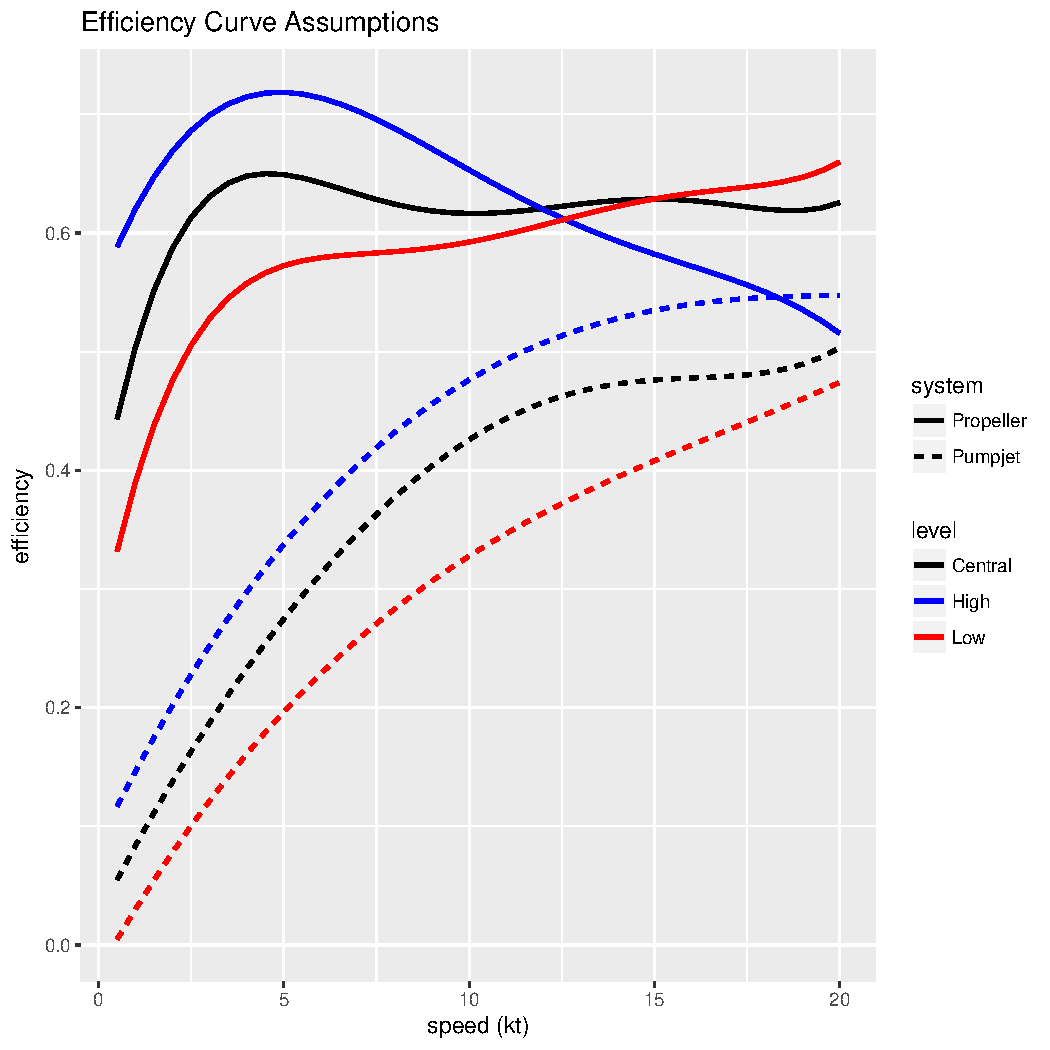
\includegraphics[width=\maxwidth]{figures/plots-plot_efficiency-1} 

}



\end{knitrout}
\caption{A range of possible efficiency curves for pumpjets and propellers to be modeled}
\label{fig:Efficiency_assumptions}
\end{figure}

\subsection{Hotel Load Assumptions}
It is also required that some assumptions are made about the hotel load, or the power which the submarine requires which doesn't go to propulsion.  We might assume that this is in the order of 100kw, as suggested in \cite{martinez1995} though official sources of information are few.  It is also likely that the actual hotel load varies considerably as different systems are switched on and off, some of which might be discretionary in combat scenarios (e.g. hot water for washing), and others (such as the combat systems) might have increased demand during crucial phases of combat operations.  It is important to note that the combat system that has been selected for Australias FSM, the AN/BYG-1, is designed for a nuclear submarine, and is reportedly consumes considerably more power than other systems \cite{muir2015}, apparently even in the order of 100kW more. \cite{patrick2011}.  Consequently, the actual hotel load experienced might vary considerably, and as such the model used in the app allows the hotel load assumption to be varied, in order to test sensitivity to this parameter.  A flat 100kW hotel load is used as a starting assumption in the initial calculations in this paper, and some sensitivity analysis is given at half and double this power, to given an indication of the impact of plausible alternative energy demands dependent on operational circumstances, and choice of combat system.

\subsection{Battery Assumptions}
Since the purpose of the task at hand is to assess dived endurance only, this model focuses on a single energy store simulated by a total embarked mass (battery bank) and an energy density of those batteries.  Since the SEA 1000 project has elected not to use lithium electric batteries, the energy density of the batteries can be assumed to be that of lead-acid batteries, which are known to be in the region of 30-50Wh/kg (Watt-hours per kilogram).  Taking a central figure and converting this to Megajoules per kilogram (MJ/kg) we assume 0.14MJ/kg to be the effective energy density of lead acid batteries for our test submarine's purposes.  This parameter can be adjusted easily for sensitivity testing, and in our case this will be adjusted to half, and double this energy density, noting that lead-acid batteries become much slower to charge as their charge level passes 80\%, and consequently it may be the case that only 50\% of their available capacity might be genuinely available for tactical purposes \parencite{briggs2016}.

It is worthwhile considering that alternative types of battery may be on offer for submarines.  In particular, lithium ion batteries were offered by TKMS in their bid for SEA 1000, and are being installed in Type 212 submarines operated by the German navy, as well as contracted for the new Norwegian submarines, as well as Israeli submarines. Precise energy density of these batteries is not publically available.  For domestic uses such as handheld electronics or solar power applications, lithium ion batteries may have 3-5 times the energy density of lead-acid batteries.  However, the actual useful density of lithium ion batteries can vary widely depending on different chemistries and designs.  It might be assumed that for very large battery banks (such as submarines) where the stability of the battery bank is of critical importance, maximum density migth be sacrificed in favour of additional safety systems, such as increased monitoring, as well as spacing and insulation barriers between cells, in order to prevent thermal runaway in one cell leading to a catastrophic fire.  The realistic energy density advantage that might be obtained as been suggested to lying closer to a factor of two \parencite{greenfield2016}.

The total embarked load of the batteries is not a well-known public figure, though it is likely to be several hundred tonnes in order to provide the likely desired levels of dived endurance.  It has been suggested publically that the approximately 700 tonnes might be required for the Shortfin Barracuda \parencite{ohff2017}.  This would appear to be quite a large fraction of the plausible payload of a submarine, even of over 4000 tonnes displacement, given that a great deal of the potential displacement will be taken by the thick steel involved in constructing a pressure vessel (probably at least a thousand tonnes per submarine) \parencite{jean2017}.  500 tonnes of batteries has been assumed as a nominal figure for these purposes.  Given that the mass of batteries embarked has only a direct and linear relationship with the dived range and endurance, no sensitivity testing will be undertaken on this variable.  Proportional changes to the energy density of the batteries will have equivalent effect for the purposes of measuring the impact on performance. Consideration of likely impacts on space, and hull-resizing, and associated drag are beyond the scope of this paper.

\subsection{Drag Coefficient of Hull}

In the online version of the web-app, alternative reference points or known facts relating a given power output to a speed can be used in order to solve for this constant $C_d$.  For instance, one might assume (as done by \cite{davies2017}) that the hotel load might match the propulsive demand at some given speed, for some given hotel load.  However, given that the precise hotel load is generally not known, and highly variable, and there is potential for the different systems to have widely varying propulsive efficiencies at low speeds, this method is subject to very wide error margins.

Given that any known power consumption level and speed match can be used as a reference, I have chosen instead to use the probable power consumptio at top speed, both of which we have some indication of, and given that propulsive efficiencies of the two systems are likely to be much closer at this speed, there will be less error in likely comparisons between different design concepts.  It is known that the a early German designs for a plausible submarine for SEA 1000 included a 6MW electric motor \parencite{patrick2012}, and the Shortfin Barracuda of Naval Group is often referred to as having a 7MW electric motor \parencite{ohff2017} \parencite{coates2016}, with top speeds ">20kt".  Given the nature of increasing drag at high speeds, it seems unlikely that top speeds will be very far above 20kt. Hence, in this model we have assumed that 20kt will be obtained with the ouput of 6.5MW.

\section{Results and Discussion}

\subsection{Power Demand}
As part of the calculation of results for each pair of efficiency curves, the power requirements of each respective component (propulsion for the two respective systems, as well as effective power required, and hote load) can be plotted to ensure that realistic results are obtained, which is important for selecting plausible values for the constant $C_d$.  For the central efficiency curves, we can show the resultant power curves for the the assumed values of battery load, energy density, and hotel load, as seen in Figure \ref{fig:power_curve}.


\begin{figure}
\begin{knitrout}
\definecolor{shadecolor}{rgb}{0.969, 0.969, 0.969}\color{fgcolor}

{\centering 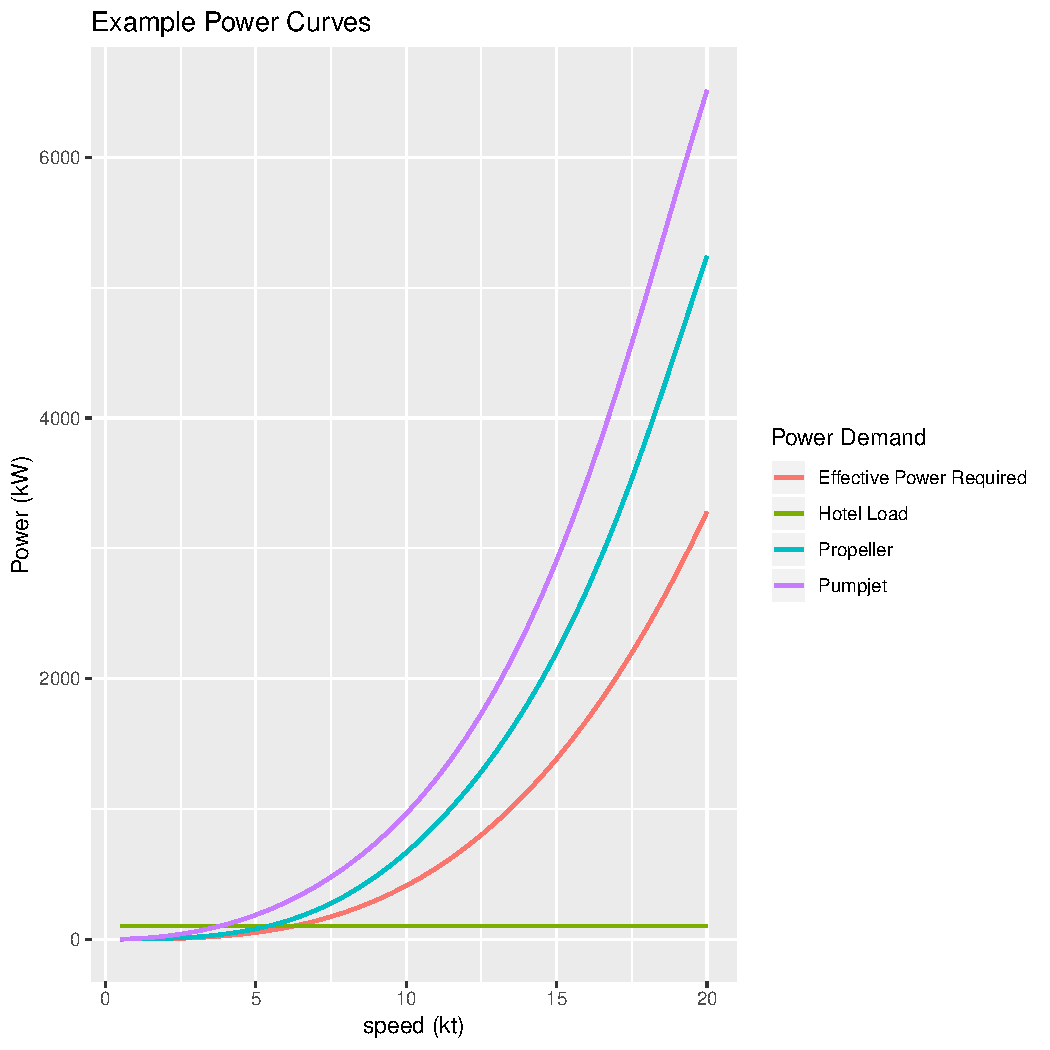
\includegraphics[width=\maxwidth]{figures/plots-plot_power1-1} 

}



\end{knitrout}
\caption{With central assumptions, a pumpjet powered submarine reaches 20kt with 6.5MW of delivered power.  Hotel load matches propulsion power demand around or below 5kt.}
\label{fig:power_curve}
\end{figure}

It can be seen here that one of Andrew Davies assumptions, regarding hotel load matching propulsion power demand at patrol speeds, might match quite closely with our assumptions at a patrol speed of 4kt for the case of a pumpjet.  It also shows the remarkable impact of the square law on power demands, particularly their effect at low speeds.  At just a few kt, an entire submarine might be propelled by a power level comfortably produced by a large family car.  This gives further explains why it is that efficiencies of propulsion systems aren't routinely discussed at dramatically lowered speeds. Even for jets which have efficiencies which decline much faster than those we've assumed (for example in \cite{fujisawa1995}), the reduction in power demanded falls substantially faster than efficiency.  Consequently, at low speeds nothing dramatic occurs to make the declining efficiencies of consequence to operators. It is often still more economical for such vessels to travel very slowly, well outside the ideal performance range of their propulsion systems, simply because of the drag on the hull.

Overall, this chart is consistent with expectation, and confirms that a plausible value of $C_d$ has been selected under these assumptions.

\subsection{Central Results}
The plots comparing the resultant endurance and range calculations across the speed range considered are in Figures \ref{fig:central_extreme}, \ref{fig:central_jet}, \ref{fig:central_prop} and \ref{fig:bottom_top}.  In all cases, the comparison for the central efficiency curves have been replotted centrally, in order to highlight varience under each of the different assumption comparisons.

It is clear that under the central assumptions, the declining efficiency of the pumpjet has a very significant impact on range and endurance, particularly at speeds around 4-8kt. It might be noted that under the central assumption, the propeller system achieves 138 hours of dived endurance at 4kt where the pumpjet only manages 91 hours dived endurance at this speed.  Consequently, at a likely patrol speed, the difference amounts of almost exactly two days in dived endurance. One might presume that such a difference is of some considerable tactical significance.  In order to match the propeller's dived endurance, the pumpjet submarine would need to slow to 2.5kt.

The phenomenon manifests itself in a very substantial reduction in the overall range that can be achieved submerged, and a difference between the speed at which maximum range can be achieved.  Under central assumptions, the propeller driven submarine can reach over 540nm, at any speed between 4 and 5kt. The pump-jet driven submarine reaches over 360nm between 3 and 6kt. A difference 180nm dived range would presumeably be of considerable tactical significance.



\begin{figure}
\begin{knitrout}
\definecolor{shadecolor}{rgb}{0.969, 0.969, 0.969}\color{fgcolor}

{\centering 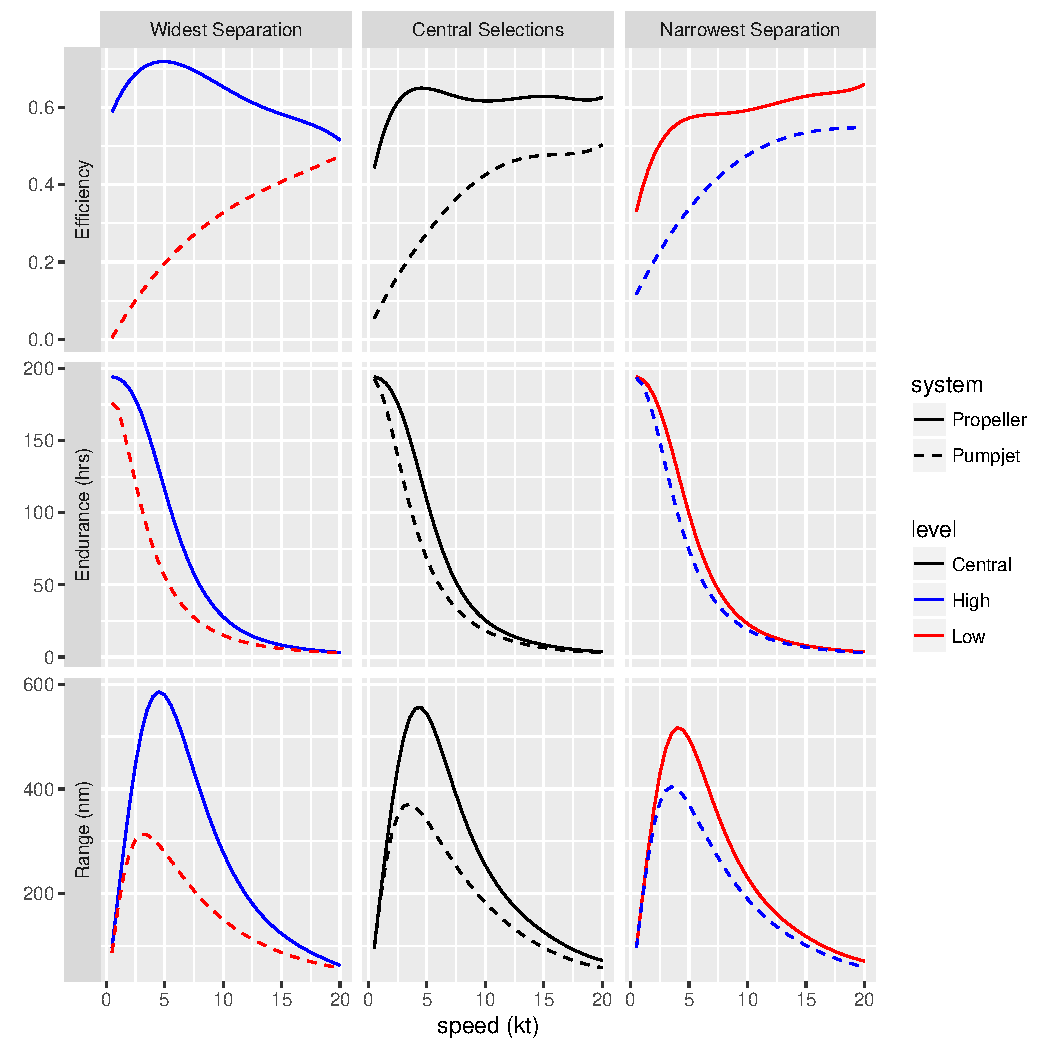
\includegraphics[width=\maxwidth]{figures/plots-plot_results1-1} 

}



\end{knitrout}
\caption{The most extreme and central assumptions are compared}
\label{fig:central_extreme}
\end{figure}

\begin{figure}
\begin{knitrout}
\definecolor{shadecolor}{rgb}{0.969, 0.969, 0.969}\color{fgcolor}

{\centering 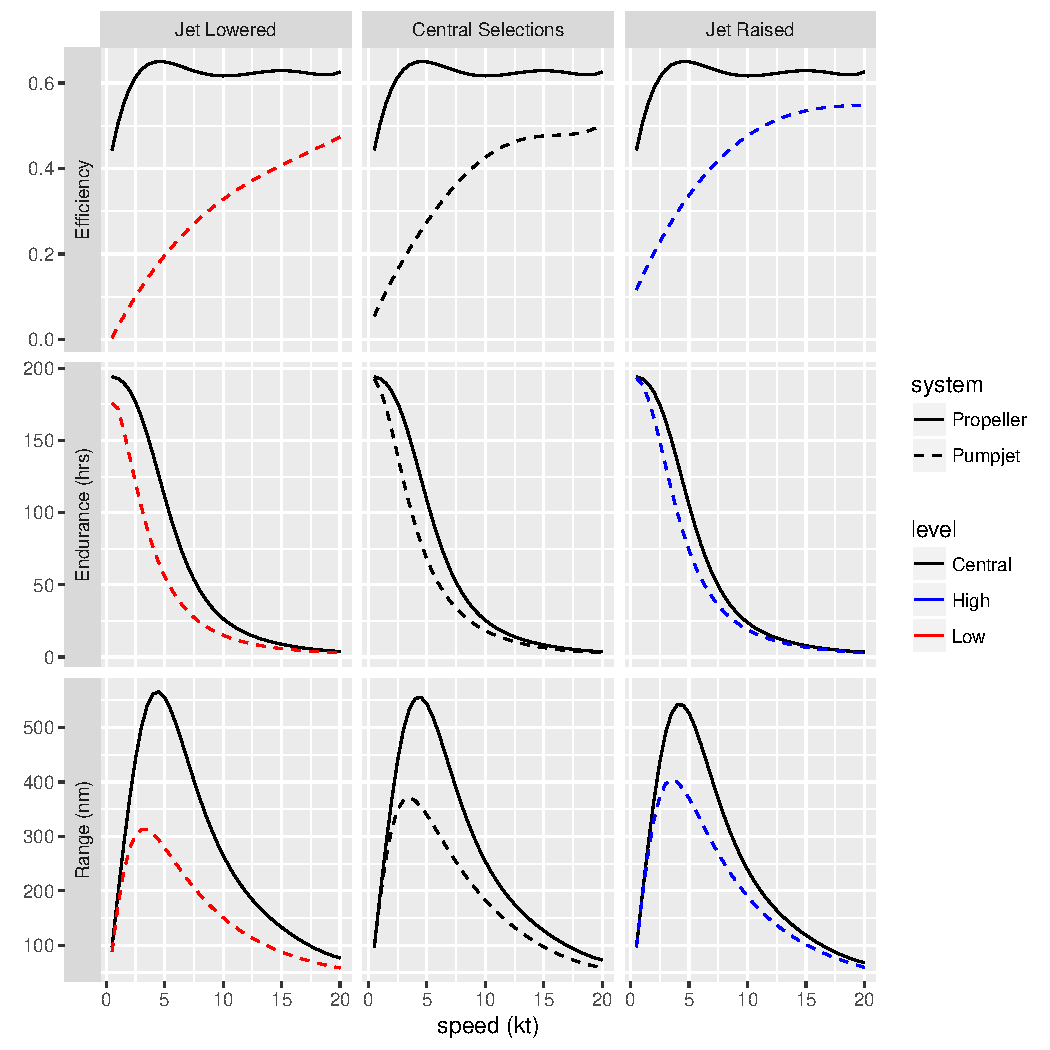
\includegraphics[width=\maxwidth]{figures/plots-plot_results2-1} 

}



\end{knitrout}
\caption{The impact of different jet efficiency assumptions compared to the central propeller curve shows wide variance}
\label{fig:central_jet}
\end{figure}

\begin{figure}
\begin{knitrout}
\definecolor{shadecolor}{rgb}{0.969, 0.969, 0.969}\color{fgcolor}

{\centering 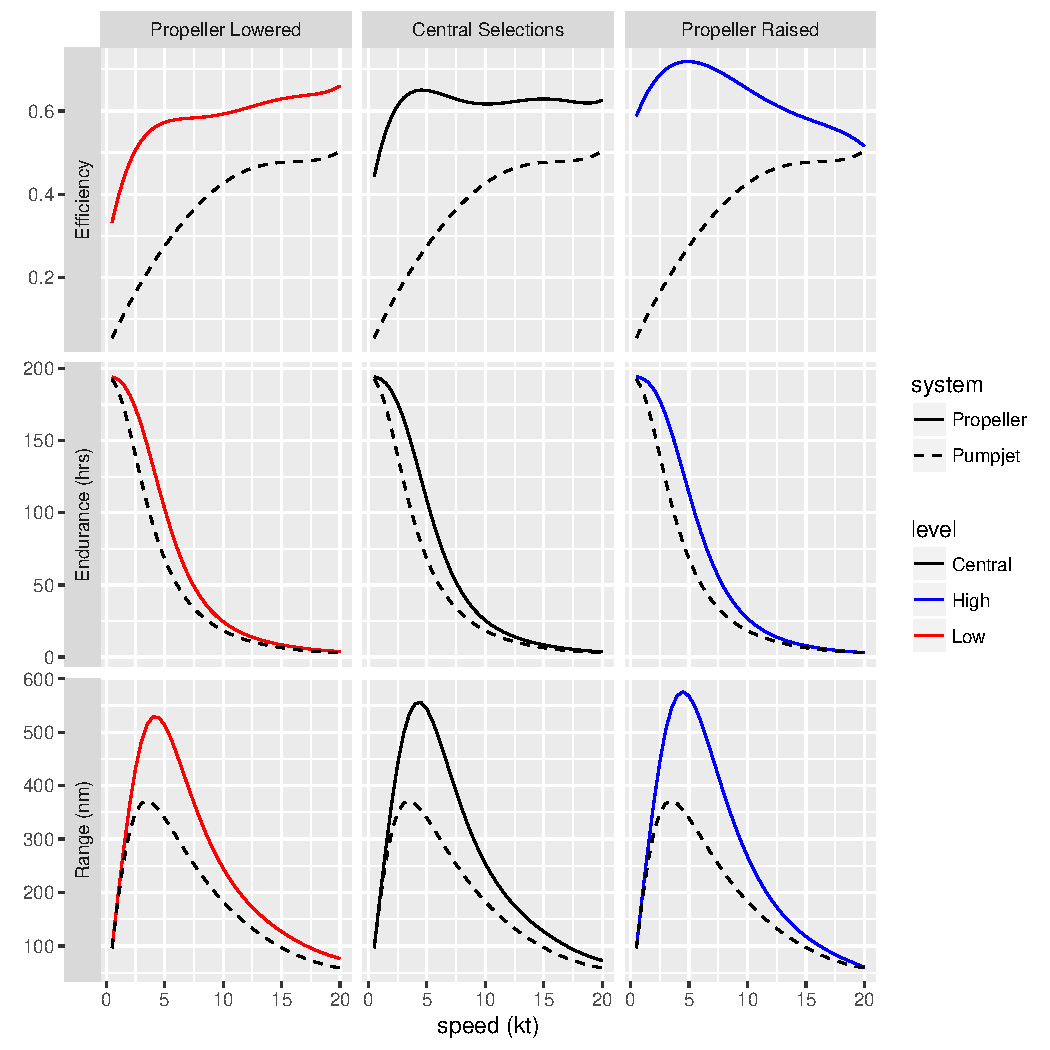
\includegraphics[width=\maxwidth]{figures/plots-plot_results3-1} 

}



\end{knitrout}
\caption{The impact of different propeller efficiency assumptions compared to the central pumpjet curve shows less variance}
\label{fig:central_prop}
\end{figure}

\begin{figure}
\begin{knitrout}
\definecolor{shadecolor}{rgb}{0.969, 0.969, 0.969}\color{fgcolor}

{\centering 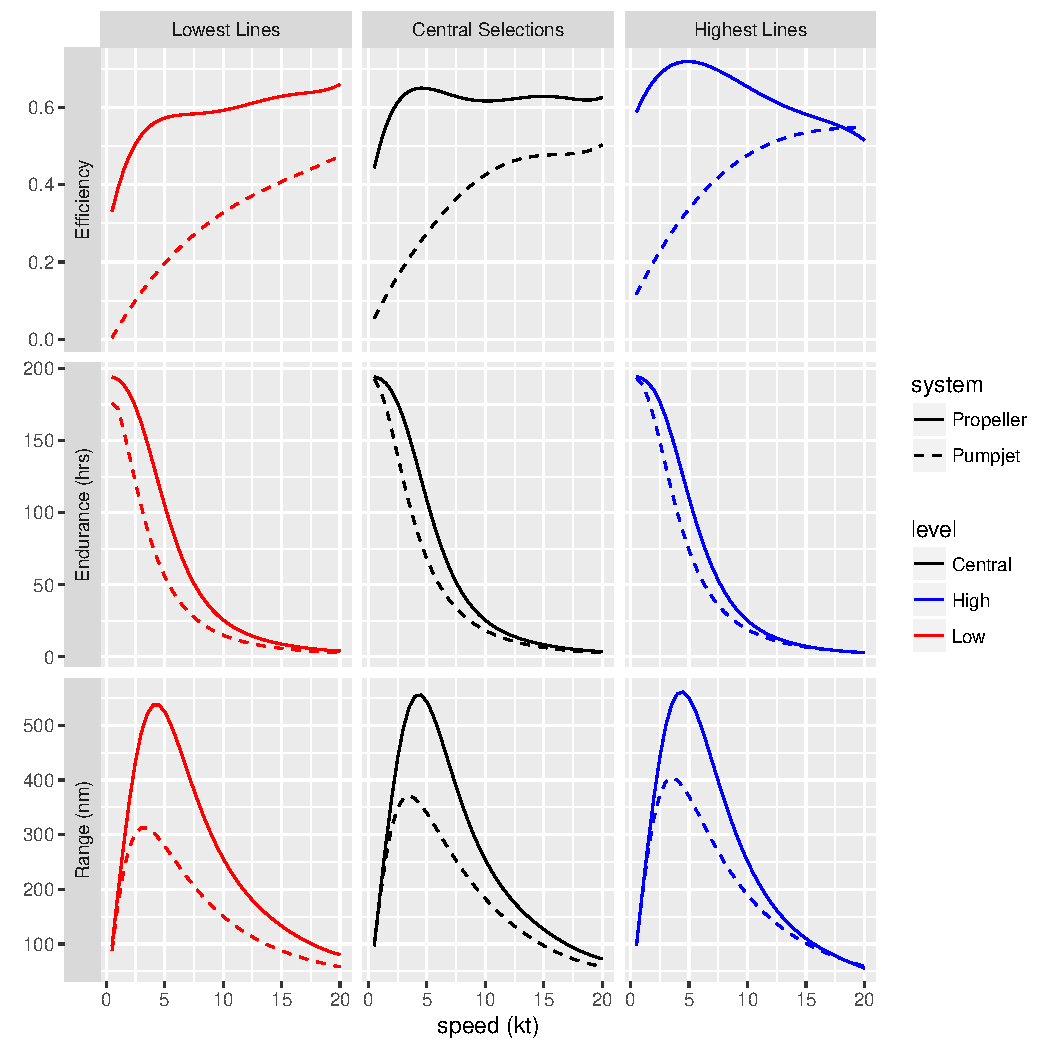
\includegraphics[width=\maxwidth]{figures/plots-plot_results4-1} 

}



\end{knitrout}
\caption{Comparing the lower and higher lines for both systems together}
\label{fig:bottom_top}
\end{figure}

\subsection{Sensitivity of Curve Selection}
As can be seen from the comprehensive comparison in Figures \ref{fig:central_extreme}, \ref{fig:central_jet}, \ref{fig:central_prop} and \ref{fig:bottom_top}, the shape of curves selected has very different levels of impact at different speeds.  Key observations include how small the impact of efficiency variation to eithre curves tends to be at very low speeds (under 2kt).  This is due to hotel load becoming clearly dominant at such speeds.  The relative difference between the lines also diminishes somewhat towards higher speeds.  More striking, however, is the very dramatic reduction in both range and endurance at higher speeds. At a speed of 20kt, a propeller driven sumbarine might manage to remain dived for 3.6 hours according to these assumptions, where a pumpjet driven submarine might manage just under 3 hours.  A difference of about half an hour would presumeably be of less tactical significance. At any speed above 10kt, neither submarine would be able to remain dived for much more than 24 hours (25.4 hours for the propeller system, 18.3 for the jet).

It should also be noted that these results, and those around 8kt, can also provide some insight into likely snorting intervals and indiscretion ratios.  As given in \cite{patrick2012}, submarines tend to carry diesel power capacity that approaches their main motor power. Whilst the difference between the two systems still appears very significant at these speeds, it appears that if transits occur in the region of 8-10kt, snorts might occurr roughly daily, and last a number of hours.  The indiscretion ratio during commute of the jet system would be significantly impaired given the substantially larger power demands at transit speeds, though a detailed calculation and comparison lies outside the scope of this paper.

It seems extremely clear from these conclusions that the general results confirm very strongly that the impact of the propulsion system is likely to be of the greatest importance in the speed range 3-8kt, where propulsion power is more significant relative to hotel load, but excessive drag does not prohibit significant dives.

A further feature of the results is that the relative difference in performance is much more sensitive to changes in the efficiency of the jet at the relevant speeds, owing to their larger proportional impact at low efficiencies.  Whilst a smoothly declining curve from around or over 50\% at 20kt to zero at 0kt, the precise path taken, particularly the exact level around 3-8kt, is of great importance, substantially more than plausible variations in the propeller curve.  This can be seen in an overlaid plot of the proportional differences in total power demand (hence endurance and range) for the different pairs of curves as in Figure \ref{fig:all_proportions}.

\begin{figure}
\begin{knitrout}
\definecolor{shadecolor}{rgb}{0.969, 0.969, 0.969}\color{fgcolor}

{\centering 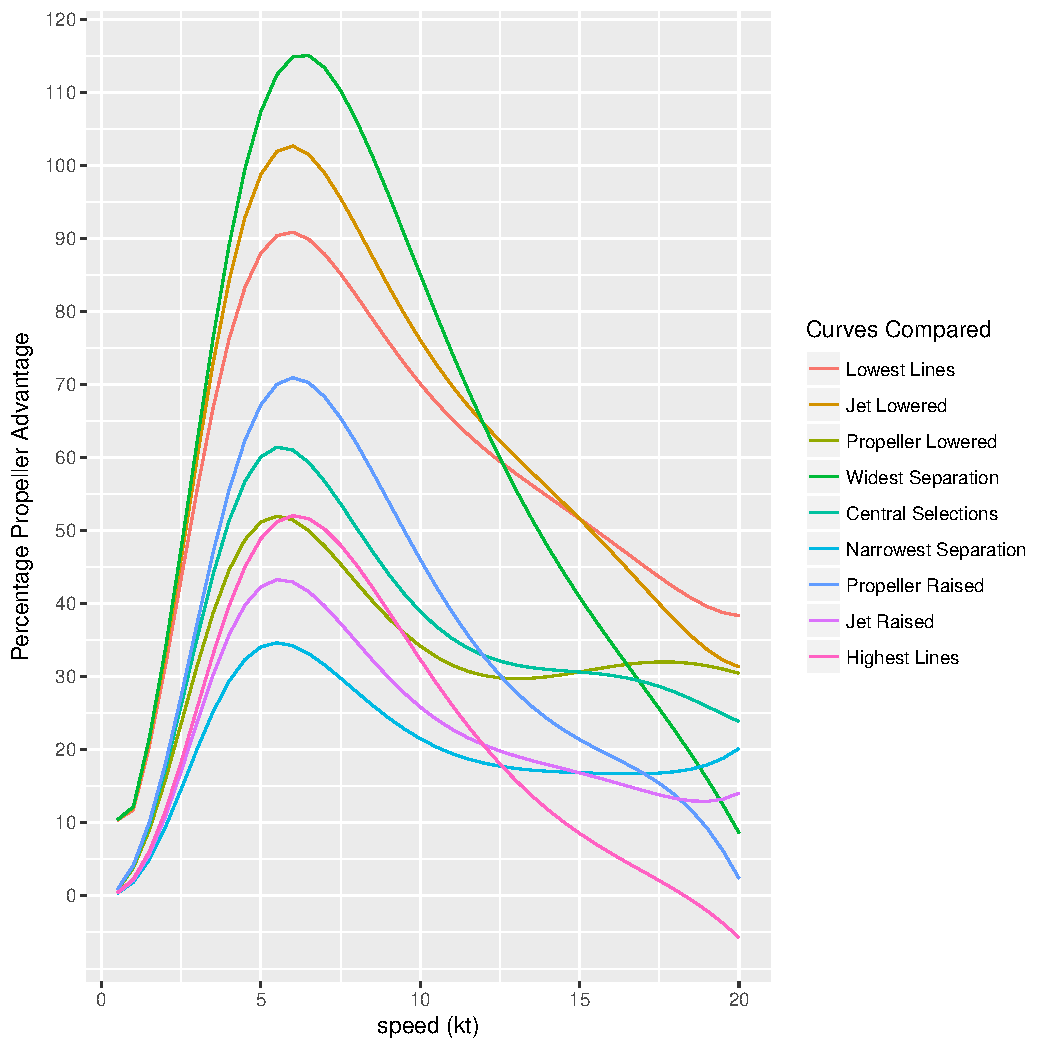
\includegraphics[width=\maxwidth]{figures/plots-plot_proportions-1} 

}



\end{knitrout}
\caption{The most proportional differences between the propeller and pumpjet performances for a range of assumptions}
\label{fig:all_proportions}
\end{figure}

The proportional change in overall power requirement (directly determining both range and endurance) shows that our central scenario shows a propeller driven submarine would have more than 60\% advantage in terms of range and endurance around 5-6kt. It is interesting to note that the proportional change is greatest slightly above the speed where maximum range is achieved, and the point of peak advantage moves steadily towards higher speeds as the difference in efficiency between the systems increases.

As can be seen, even compred to the central propeller curve, choosing a jet efficiency curve somewhat lower than the central assumption means that the peak difference immediately jumps to over 100\%, or effectively allow a propeller powered submarine to achieve double the range and endurance of a pumpjet powered submarine at those speeds.  It is important to note that these speeds in include those speeds which might lie near the maximum speeds that could be sustained by Air Independent Propulsion (AIP) systems \parencite[100]{@stanford2017}.  Consequently, it is likely that a conventional submarine that used pumpjets might only achieve a fraction of the dived range and endurance enhancements generally expected on propeller powered submarines which employ this technology.

The proportional improvements will also be effective rough guides to the likely impact on indescretion ratios and overall range.\footnote{Additional considerations including the size and efficiency of the diesel engines and generators must be included for proper analyses of indescretion ratios, which will not be given here.}  Near patrol speed almost all scenarios show a difference approaching or exceeding 50\%, which will have a material impact on indescretion rates during all combat operations.

Perhaps surprisingly, the impact at transit speeds is still quite significant, with no scenarios showing less than 20\% advantage around 8-10kt. The sensitivity to pumpjet efficiency here is also very high, with three scenarios showing an impact of over 70\%.  Given the likelihood that a submarine's average speed over its range is likely to be dominated by its transit speed, this indicates that the choice of a pumpjet propulsion system will also result in a substantial reduction in the overall range of the submarine, quite probably in the range of between 25-50\%.  This would require the embarkation of significantly larger volumes of diesel to meet minimum range requirements, and also contribute to higher running costs.

\subsection{Sensitivity to Hotel Load}

\begin{figure}
\begin{knitrout}
\definecolor{shadecolor}{rgb}{0.969, 0.969, 0.969}\color{fgcolor}

{\centering 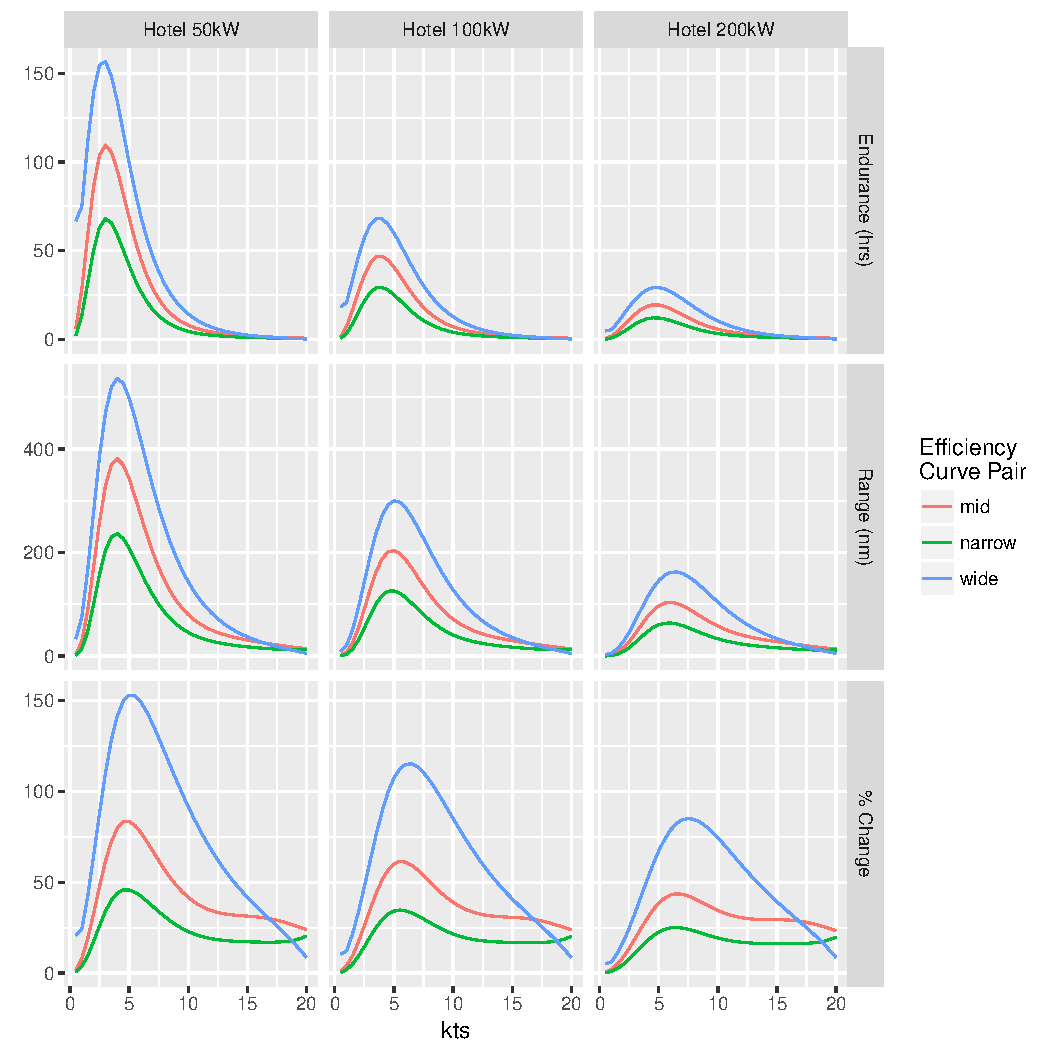
\includegraphics[width=\maxwidth]{figures/plots-plot_sens_hotel-1} 

}



\end{knitrout}
\caption{The impact of the propulsion system efficiencies are very sensitive to changes in the hotel load, including as a proportion.}
\label{fig:sens_hotel}
\end{figure}

\subsection{Sensitivity to Battery Changes}

\begin{figure}
\begin{knitrout}
\definecolor{shadecolor}{rgb}{0.969, 0.969, 0.969}\color{fgcolor}

{\centering \includegraphics[width=\maxwidth]{figures/plots-plot_sens_battery-1} 

}



\end{knitrout}
\caption{The impact of the propulsion system efficiencies are extremely sensitive to battery energy density (or load) though proportions remain fixed.}
\label{fig:sens_battery}
\end{figure}

\subsection{The interaction of hotel load, battery energy density, and efficiency curves}

\begin{figure}
\begin{knitrout}
\definecolor{shadecolor}{rgb}{0.969, 0.969, 0.969}\color{fgcolor}

{\centering \includegraphics[width=\maxwidth]{figures/plots-plot_sens_corners-1} 

}



\end{knitrout}
\caption{Specifying low density batteries and a high hotel load dramatically reduces the proportional and nominal impact of propulsion system efficiencies at low speeds}
\label{fig:sens_corners}
\end{figure}

\section{Acoustic Considerations}

\subsection{The importance of cavitation inception}
It is generally considered that the existence of cavitation of any sort will tend to dominate the acoustic signature of any vessel that doesn't produce any machinery noise by relying on all-electric drive as a conventional submarine would when dived (\cite{giles2010}, \cite{harvie1965construction}).  Its quite possible that during the period when a submarine is snorting, or running its diesel engines, these sources of noise would be a more substantial and distinctive acoustic signature than small amounts of cavitation on the propulsion system, if it were to occur, owing in particular to the low freqency of diesel engines.

Other sources of noise hydrodynamic noise, such as the turbulence produced in the boundary layer of the flow over the hull, or parts of the propulsor, will still contribute to overall noise and some signature, but it will tend to be vastly smaller in magnitude.  This owes to the essentially incompressible nature of water.  Without compression, even very relatively intense votices or tubulent flows will not propagate very much noise, if the water remains perfectly solid.  All of the 'round and round' can't achieve much 'in and out', which is what results in propagated noise.  This obviously doesn't hold true in compressible fluids, such as air, as one would observe noticing the intense noise produced by hand-dryers, aeroplanes, jet engines etc.  It also doesn't hold true within a turbulent flow underwater.  If you were to put a sensor inside a turbulent flow, the rapid movements would result in continual and significant pressure fluctuations, hence noise.  But at a distance, these fluctuations tend to substantially cancel out.  The larger the scale of the eddies and vortices, the further noise might propagate, and also the lower the frequencies of resultant noise might be, which makes noise propagate further.  Likewise, larger caviation voids will tend to emit lower frequency sound aswell, as can be observed from the boiling of a kettle.

However, when dived, it might be reasonably assumed that the complete elimination of all sources of cavitition will be the primary objective of acoustic signature management.  This is neatly put in \cite[88]{gearhart1966selection}: "The occurence of cavitation in a propulsor results in adegradation of the propulsor operating characteristics if extensive amounts of cavitation exist, and in significant noise when minute amounts occur.  As a result, the performance requirements of a submersible weapon system specify that the occurence or inception of cavitation be avoided below certain operating depths." One might consider that a submarines 'tactical silent speed' would most probably correspond to the speed at which it can operate safely below the point of any cavitation inception.


\subsection{The impact of depth on cavitation}
It is crucial to understand that increasing depth necessarily increases the static pressure throughout a propulsion system.  As such, the speed at which cavitation starts to occur, will necessarily be a function of depth.  Approximately every 10m of water adds approximately the equivalent of an atmosphere of pressure.  As such, the static pressure a system experiences at 10m depth will be half that experienced at 30m (since the air in the atmosphere comprises the first atmosphere of pressure).  Consequently, diving deeper will necessarily increase the speeds one can achieve without any cavitation occurring \ref{fig:InceptionDepth.png}.

\begin{figure}
\includegraphics[width=\textwidth]{InceptionDepth.png}
\caption{Increasing in depth improves the speed achievable before cavitation begins to occur, as shown in the case of a torpedo \parencite{suryanarayana2010cavitation}}
\label{fig:InceptionDepth.png}
\end{figure}

This relationship can be expressed in a general form in \ref{fig:InceptionContours}, which has been generated using an approxiate numeric model. As can be seen here, at very low speeds, modest changes in depths can achieve considerable additional surplus pressure in order to prevent cavitation.  However at much higher speeds, sine the pressure diffential scales with the square of the velocity travelled, far greater additional depths are required to achieve sufficient excess static to supress cavitation for a give further speed increase.

\begin{figure}
\begin{knitrout}
\definecolor{shadecolor}{rgb}{0.969, 0.969, 0.969}\color{fgcolor}

{\centering \includegraphics[width=\maxwidth]{figures/plots-plot_inception-1} 

}



\end{knitrout}
\caption{Contours showing plausible lines of plausible equivalent cavitation inception}
\label{fig:InceptionContours}
\end{figure}

\subsection{The significance of flow separation}
It is also important to understand that the addition of a duct will necessarily to flow separation occuring on the inside of the duct opening at very low speeds which correspond to high advance ratios when load remains constant.  Flow separation tends to lead to vortex shedding, which means that inconsistent flows (vortices) are then ingested into the blades of the impeller.  This effect is well known and document.  A good example is shown on the exterior of an \textbf{accelerating} duct at $J = .8$ in \cite{willemsen2013}.

\begin{figure}
\includegraphics[width=\textwidth]{VortexShedding.png}
\caption{Vortex shedding following a flow separation leads to eddies being released unsteadily into the main flow stream, as shown here on the exterior of an accelerating duct.  In the case of decelerating duct (pumpjet), duct shape is inverted, leading to the vortices being shed into the impeller blades. \parencite{willemsen2013}}
\label{fig:VortexShedding.png}
\end{figure}

Whilst at very low power levels, or at good depths, it is quite plausible that this doesn't result in any cavitation, which would normally be a likely occurrence if the blades are operating closer to their design power and such such vortices were shed into the intake.  However, given the inherently unpredictable and unsteady nation of such vortex formation and shedding, the this phenomenon would increase the risk of cavitation occurring unexpectedly in marginal conditions.  In addition, in the absence of cavitation, the sudden and changing pressure gradients over the blades would dramatically increase the overall pressure fluctuations and turbulence level that occurs within the propulsor.  This would necessarily increase the overall levels of noise generated.  It is plausible that the noise is of sufficiently small level that it is not considered a significant compromise of stealth.  In essence, the higher levels of noise lie below some threshold of significance.  However, it is almost certainly untrue that that pumpjet actually generates less noise overall than a propeller at very low speeds.

\subsection{The impact of duct shielding}
The presence of the duct around the impeller may also have the effect of preventing the noise from being effectively radiated away from the propulsor.  This may well result in substantial reductions in some types of noise being radiated away from the propulsor in certain directions, which may have given rise to the consistent qualification of 'radiated' being used to descrive the type of noise which differentiated the French submarine bid \parencite{stewart2016, davies2017, ohff2016}, including by the designers of the submarine \parencite{autret2016}.  This is a secondary effect, quite separate to the avoidance of cavitation, which might be seen as an acoustic advantage in circumstances where cavitation might not be expected to occur on either type of propulsor.  It is highly likely that this is the effect which is relied upon to sustain claims that a pumpjet is generally acoustically superior to a propeller, including at low speeds.

It should be noted here that shielding effects might comprise the combination two distinct and seperate physically phenomenon: reflection and damping.  Noise tends to be reflected very effectively off hard, smooth surfaces representing the boundary between mediums of very different density (such as steel and water).  Changes in density which are gradual, often representing soft, squishy, or broken surfaces tend, to have the effect of absorbing sound, where the acoustic energy is converted to heat or degradation of the material, rather than reflecting it.  Given the significance of increased drag on any surfaces within the propulsor, it is highly unlikely that any attempt at damping is made within the pumpjet.  However, it should be noted that some pumpjets have been constructed with a hollow design, in order to reduce weight \parencite{harvie1965construction}, which would reduce the thickness of solid steel, though offer some potential opportunity for damping.  Overall, damping is increased in its effectiveness at low frequencies by allowing it to occur over larger distances, corresponding to the sound's increased wavelenght, leading to increased thickness of the transition substance or damping material.  Consequently, effective damping within the propulsor itself is unlikely to be attempted, or limited to medium and higher frequencies, probably suited to reducing noise from normal surface flow turbulence and very early onset cavitation.

The ability of a thin layer of material to reflect noise is also highly frequecy dependent, and also dependent on mass of the shield layer.  As the material becomes thinner and thinner, a hard shield layer will tend increasinly to transmit rather than reflect the noise, a phenomenon that increases as the amplitude (loudness) of the noise increases, and frequency decreases.  Denser materials are more effective at reflecting sound, as more energy (pressure) is required to excite the same movement in the material.  Consequently, the effectiveness of a shield depends on both its thickness and density.  There is therefore some tension inherent in the design of a shield where thickness and total weight are constrained.  A thicker layer solid steel will be very effective at reflecting sound, but have negligible absoption or damping.  A hollow between two thin layers will offer some potential for a soft daping material to be inserted, but at the cost of reflection.

It is most likely that little or no damping or absorbing layer is attempted within the body of the shroud, since increasing the duct thickness above hydrodynamically determined optimum profile is likely to have a detrimental impact on efficiency.  Constructing especially thin layers, and still maintaining an optimal shape to the precision required for housing powerful turbomachinery like the impeller is also likely to involve considerable construction risk and complexity.  Hence the shielding effect is most likely to dominated by the reflective characteristics of the duct, which would seek to internally reflect noise back into the turbulent flow, where sound waves would be increasingly convoluted, and somewhat absorbed through the eventual transition to small-scale turbulence and heat.

The degree to which the total noise generated is reflected internally will also be shape-dependent.  A more concave inner surface, consistent with higher degrees of diffusion in advance of the impeller, and greater nozzle narrowing after it, which is consistent with higher pressure elevation at the impeller (hence improved cavitation characteristics) but higher negative duct thrust, leading to even poorer efficiencies at low speed.  Substantial alteration of duct shape on account of efficiency considerations at low speed are therefore necessarily going to have some impact on the degree of effective shielding that a duct can afford.

\subsubsection{Directional Dependence}
Two important qualifications must be made regarding shielding.  The first is that its impact is highly directionally dependent.  The pump jet requires openings at the front and back to allow water in and out. Only noise that is reflected internally sufficient to be largely absorbed is effectively shielded.  The larger the areas of the intakes and outlets, the narrower the effective shielding will become.  Consequently, design changes to make the pump more efficient at low speeds, which may include expanding both the inlet and outlent, and diminshing the difference between them, will necessarily be at the expense of diminishing effective width of the shielding 'belt' around the propulsor.

When the submarine is travelling at high speeds, and there is significant flow through the propulsor, the impact of waterspeed through the propulsor might have the additional impact of diminishing the radiation of noise in the forwards direction, in the same way that sound tends tends not to travel well up-wind in air.  However, at very low speeds this effect would be greatly diminished.

It should be noted that in the underwater environment sound can be made to reflect in a variety of directions simply with differences in temperature, salinity, movement, as well as off plenty of nearby underwater objects, including the ocean floor and objects on it.  This phenomenon generally serves to make the art of underwater acoustics extremely complex and unpredictable, and generally contributes to the difficulty of precisely locating a submarine, even when some signature is detected.  However, it also means that direction-dependent reductions signature do not reliably translate to overall reduced probability of detection.

\subsubsection{Frequency Dependence}
It ought further to be noted that the effectiveness of acoustic shielding is also highly dependent on frequency.  Much lower frequencies are very hard to reflect, and absorb, as can be easily observed in a house with a home-cinema, where lower frequencies emitted by the subwoofer will tend to affect many surrounding rooms, where higher frequency sounds might be substantially muffled by interceding walls. The same acoustic effects are at work in underwater acoustics.

This has an important consequence for shielding for pumpjets at very low speeds because of the occurrence of flow separation and vortex shedding. In the absence of flow separation, and cavitation at very low speeds the most substantial sources of sound would be the turbulent flow over surfaces of in the propulsor.  This noise will tend to be relatively white and high in its frequency owing to the very small length-scales of the eddies and vortices in such turbulence.  The steel shroud would be very effective in reflecting such high frequency noise.  Under acceleration or higher loads, the very instances of cavitation woud also be relatively high frequency, as the voids or cavities would be small at first. These sounds might also be very effectively reflected by the shroud, and consequently diminished.  However, flow separation results in the creation of vortices of a dramatically larger scale than occurs with normal turbulence in a boundary later, and hence generate noise of a much lower frequency.  In addition, as the flow rates slow even further, these vortices are likely to become larger in size, even if lesser in intensity, resulting in further reduction in the frequency of noise generated.  Further to this effect, the rate at which the vortices shed from the surface and impact the impeller will also result in another acoustic signature, of even lower frequency.  Again, at lower flow rates, these vortices will tend to develop and shed more slowly, lowering frequencies further.

Consequently, whilst for certain types of noise which tend to become both louder and lower in frequency with increasing speed (cavitation), flow separation provides a contrasting characteristic, in that it is likely to decrease in frequecy with decreasing speed.  As lower frequencies tend to propagate much further in open water, this could have a significand adverse impact on the total acoustic signature of the submarine, even if the flow separation doesn't lead to any cavitation.

The foregoing consideration suggests that the acoustic signature of a jet-powered submarine might not reduce steadily with speed all the way to stationary movement.  It is plausible that there could be some elevated propulsion signature at very low speeds due to flow separation, and that the submarine's optimal acoustic signature when moving is actually at some slightly higher speed, where smoother flow through the propulsor can be achieved.  However, given that the amplitude, frequency, and combined impact of those two characteristics cannot be accurately evaluated without substantial further work and more detailed system knowledge, it is also possible that the increase in other noise (including hull flow noise and other machinery) at elevated speeds offsets the improvement in the smoothness of the pumpjet's operation.  It is also possible that the overall level of noise radiated by the pumpjet, including under conditions when flow separation occurs, is still considered to be sufficiently low as to not be of significant tactical consequence.  However it is highly unlikely that the accoustic signature of the pumpjet is actually superior to that of an open propeller at very low speeds, when cavitation occurs for neither system, but substantially increased turbulence including flow separation must neccessarily occur for the pumpjet.

\section{Conclusions}
This is a pretty bad result for the pumpjet.

\printbibliography

\end{document}
